% (unofficial) La Trobe PhD Thesis Template
% Copyright (C) 2018 Matthias Langer
%
% This program is free software; you can redistribute it and/or modify
% it under the terms of the GNU General Public License as published by
% the Free Software Foundation; either version 2 of the License, or
% (at your option) any later version.
%
% This program is distributed in the hope that it will be useful,
% but WITHOUT ANY WARRANTY; without even the implied warranty of
% MERCHANTABILITY or FITNESS FOR A PARTICULAR PURPOSE.  See the
% GNU General Public License for more details.
%
% You should have received a copy of the GNU General Public License along
% with this program; if not, write to the Free Software Foundation, Inc.,
% 51 Franklin Street, Fifth Floor, Boston, MA 02110-1301 USA.
%
\documentclass[oneside,openright,titlepage,numbers=noenddot,headinclude,footinclude=true,cleardoublepage=empty,listof=totoc,paper=a4,fontsize=11pt,american,BCOR=5mm]{scrreprt}

% -----------------------------------------------------------------------------
%   CONFIGURATION
% -----------------------------------------------------------------------------
% Thesis and submission:
\newcommand{\myTitle}{Anomaly detection for the real-time identification of gamma-ray transients}
\newcommand{\mySubmissionYear}{2023}
\newcommand{\mySubmissionMonth}{January}
\newcommand{\mySubmissionDay}{31}

% Regarding yourself:
\newcommand{\myFirstName}{Leonardo}
\newcommand{\myLastName}{Baroncelli}
\newcommand{\myWebsite}{}
\newcommand{\myBirthYear}{1989}
\newcommand{\myBirthMonth}{November}
\newcommand{\myBirthDay}{02}
\newcommand{\myBirthPlace}{Bagno a Ripoli (Firenze)}

% Primary supervisor:
\newcommand{\myProfTitle}{Dr.}
\newcommand{\myProfFirstName}{Andrea}
\newcommand{\myProfLastName}{Bulgarelli}
\newcommand{\myProfWebsite}{}

% Co-supervisor:
\newcommand{\myOtherProfTitle}{Prof.}
\newcommand{\myOtherProfFirstName}{Antonio}
\newcommand{\myOtherProfLastName}{Zoccoli}
\newcommand{\myOtherProfWebsite}{https://www.unibo.it/sitoweb/antonio.zoccoli}

% University related:
\newcommand{\myDepartment}{Dipartimento di Fisica e Astronomia}
\newcommand{\myFaculty}{College of Science, Health and Engineering}
\newcommand{\mySchool}{Data Science and Computation}
\newcommand{\myUni}{Università di Bologna}
% -----------------------------------------------------------------------------

% ****************************************************************************************************
% classicthesis-config.tex 
% formerly known as loadpackages.sty, classicthesis-ldpkg.sty, and classicthesis-preamble.sty 
% Use it at the beginning of your ClassicThesis.tex, or as a LaTeX Preamble 
% in your ClassicThesis.{tex,lyx} with % ****************************************************************************************************
% classicthesis-config.tex 
% formerly known as loadpackages.sty, classicthesis-ldpkg.sty, and classicthesis-preamble.sty 
% Use it at the beginning of your ClassicThesis.tex, or as a LaTeX Preamble 
% in your ClassicThesis.{tex,lyx} with % ****************************************************************************************************
% classicthesis-config.tex 
% formerly known as loadpackages.sty, classicthesis-ldpkg.sty, and classicthesis-preamble.sty 
% Use it at the beginning of your ClassicThesis.tex, or as a LaTeX Preamble 
% in your ClassicThesis.{tex,lyx} with \input{classicthesis-config}
% ****************************************************************************************************  
% If you like the classicthesis, then I would appreciate a postcard. 
% My address can be found in the file ClassicThesis.pdf. A collection 
% of the postcards I received so far is available online at 
% http://postcards.miede.de
% ****************************************************************************************************
% !!! ATTENTION !!! ATTENTION !!! ATTENTION !!! ATTENTION !!!
% This version was modified to comply with the formatting guidelines
% of the Graduate Research School of La Trobe University.
% ~ October 2018 / Matthias Langer (https://github.com/bashimao/ltu-thesis)
% !!! ATTENTION !!! ATTENTION !!! ATTENTION !!! ATTENTION !!!
% ****************************************************************************************************


% ****************************************************************************************************
% 0. Set the encoding of your files. UTF-8 is the only sensible encoding nowadays. If you can't read
% äöüßáéçèê∂åëæƒÏ€ then change the encoding setting in your editor, not the line below. If your editor
% does not support utf8 use another editor!
% ****************************************************************************************************
\PassOptionsToPackage{utf8}{inputenc}
	\usepackage{inputenc}


% ****************************************************************************************************
% 1. Configure classicthesis for your needs here, e.g., remove "drafting" below 
% in order to deactivate the time-stamp on the pages
% ****************************************************************************************************
\PassOptionsToPackage{eulerchapternumbers,listings,pdfspacing,subfig,beramono,dottedtoc}{classicthesis}
% ********************************************************************
% Available options for classicthesis.sty 
% (see ClassicThesis.pdf for more information):
% drafting
% parts nochapters linedheaders
% eulerchapternumbers beramono eulermath pdfspacing minionprospacing
% tocaligned dottedtoc manychapters
% listings floatperchapter subfig
% ********************************************************************


% ****************************************************************************************************
% 2. Personal data and user ad-hoc commands
% ****************************************************************************************************
% moved to thesis.tex


% ********************************************************************
% Setup, finetuning, and useful commands
% ********************************************************************
\newcounter{dummy} % necessary for correct hyperlinks (to index, bib, etc.)
\newlength{\abcd} % for ab..z string length calculation
\providecommand{\mLyX}{L\kern-.1667em\lower.25em\hbox{Y}\kern-.125emX\@}
\newcommand{\ie}{i.\,e.\ }
\newcommand{\Ie}{I.\,e.\ }
\newcommand{\eg}{e.\,g.\ }
\newcommand{\Eg}{E.\,g.\ }
% ****************************************************************************************************


% ****************************************************************************************************
% 3. Loading some handy packages
% ****************************************************************************************************
% ******************************************************************** 
% Packages with options that might require adjustments
% ******************************************************************** 
\PassOptionsToPackage{american}{babel}
  \usepackage{babel}

\usepackage{csquotes}
\PassOptionsToPackage{%
  backend=bibtex,
  bibencoding=ascii,
  language=auto,
  style=alphabetic,
  sorting=nyt,
  maxbibnames=10,
  natbib=true
}{biblatex}
  \usepackage{biblatex}

\PassOptionsToPackage{fleqn}{amsmath}       % math environments and more by the AMS 
  \usepackage{amsmath}

% ******************************************************************** 
% General useful packages
% ******************************************************************** 
\usepackage{amssymb}
\usepackage{lipsum}
\PassOptionsToPackage{T1}{fontenc} % T2A for cyrillics
    \usepackage{fontenc}
\usepackage{textcomp} % fix warning with missing font shapes
\usepackage{scrhack} % fix warnings when using KOMA with listings package  
\usepackage{xspace} % to get the spacing after macros right
\usepackage{mparhack} % get marginpar right
%\usepackage[latest]{latexrelease} % will be used once available in more distributions (ISSUE #107)
\PassOptionsToPackage{printonlyused,smaller}{acronym}
  \usepackage{acronym} % nice macros for handling all acronyms in the thesis
  %\renewcommand{\bflabel}[1]{{#1}\hfill} % fix the list of acronyms --> no longer working
  %\renewcommand*{\acsfont}[1]{\textsc{#1}}
  \renewcommand*{\aclabelfont}[1]{\acsfont{#1}}
% ****************************************************************************************************


% ****************************************************************************************************
% 4. Setup floats: tables, (sub)figures, and captions
% ****************************************************************************************************
\usepackage{tabularx} % better tables
\setlength{\extrarowheight}{3pt} % increase table row height
\newcommand{\tableheadline}[1]{\multicolumn{1}{c}{\spacedlowsmallcaps{#1}}}
\newcommand{\myfloatalign}{\centering} % to be used with each float for alignment
\usepackage{makecell}
\usepackage{multirow}
\usepackage[width=.75\textwidth]{caption}
% Thanks to cgnieder and Claus Lahiri
% http://tex.stackexchange.com/questions/69349/spacedlowsmallcaps-in-caption-label
% [REMOVED DUE TO OTHER PROBLEMS, SEE ISSUE #82]    
%\DeclareCaptionLabelFormat{smallcaps}{\bothIfFirst{#1}{~}\MakeTextLowercase{\textsc{#2}}}
%\captionsetup{font=small,labelformat=smallcaps} % format=hang,
\captionsetup{font=small} % format=hang,
\usepackage{subfig}
% ****************************************************************************************************


% ****************************************************************************************************
% 5. Setup code listings
% ****************************************************************************************************
\usepackage{listings}
%\lstset{emph={trueIndex,root},emphstyle=\color{BlueViolet}}%\underbar} % For special keywords
\lstset{language=[LaTeX]Tex,%C++,
  morekeywords={PassOptionsToPackage,selectlanguage},
  keywordstyle=\color{RoyalBlue},%\bfseries,
  basicstyle=\small\ttfamily,
  %identifierstyle=\color{NavyBlue},
  commentstyle=\color{Green}\ttfamily,
  stringstyle=\rmfamily,
  numbers=left,
  numberstyle=\scriptsize,%\tiny
  stepnumber=5,
  numbersep=8pt,
  showstringspaces=false,
  breaklines=true,
  %frameround=ftff,
  %frame=single,
  belowcaptionskip=.75\baselineskip
  %frame=L
}
% ****************************************************************************************************             


% ****************************************************************************************************
% 6. PDFLaTeX, hyperreferences and citation backreferences
% ****************************************************************************************************
% ********************************************************************
% Using PDFLaTeX
% ********************************************************************
\PassOptionsToPackage{pdftex,hyperfootnotes=false,pdfpagelabels}{hyperref}
\usepackage{hyperref}  % backref linktocpage pagebackref
\pdfcompresslevel=9
\pdfadjustspacing=1
\PassOptionsToPackage{pdftex}{graphicx}
    \usepackage{graphicx} 


% ********************************************************************
% Hyperreferences
% ********************************************************************
\hypersetup{breaklinks=true}
\hypersetup{linktocpage=true}
\hypersetup{colorlinks=true}
\hypersetup{urlcolor=webbrown}
\hypersetup{linkcolor=RoyalBlue}
\hypersetup{citecolor=webgreen}
\hypersetup{pageanchor=true}
\hypersetup{plainpages=false}
%\hypersetup{bookmarksnumbered=true}
%\hypersetup{bookmarksopen=true}
%\hypersetup{bookmarksopenlevel=true}
%hypertexnames=true, nesting=true, frenchlinks
\hypersetup{pdfstartpage=3}
\hypersetup{pdfstartview=FitV}
\hypersetup{pdfpagemode=UseNone}
\hypersetup{pageanchor=true}
\hypersetup{pdfpagemode=UseOutlines}
\hypersetup{pdftitle={\myTitle}}
\hypersetup{pdfauthor={\textcopyright\ \myFirstName\ \myLastName, \myUni, \myFaculty}}
\hypersetup{pdfsubject={}}
\hypersetup{pdfkeywords={}}
\hypersetup{pdfhighlight=/O}


% ********************************************************************
% Setup autoreferences
% ********************************************************************
% There are some issues regarding autorefnames
% http://www.ureader.de/msg/136221647.aspx
% http://www.tex.ac.uk/cgi-bin/texfaq2html?label=latexwords
% you have to redefine the makros for the 
% language you use, e.g., american, ngerman
% (as chosen when loading babel/AtBeginDocument)
% ********************************************************************
\makeatletter
\@ifpackageloaded{babel}%
{%
  \addto\extrasamerican{%
    \renewcommand*{\figureautorefname}{Figure}%
    \renewcommand*{\tableautorefname}{Table}%
    \renewcommand*{\partautorefname}{Part}%
    \renewcommand*{\chapterautorefname}{Chapter}%
    \renewcommand*{\sectionautorefname}{Section}%
    \renewcommand*{\subsectionautorefname}{Section}%
    \renewcommand*{\subsubsectionautorefname}{Section}%
  }%
  \addto\extrasngerman{%
    \renewcommand*{\paragraphautorefname}{Absatz}%
    \renewcommand*{\subparagraphautorefname}{Unterabsatz}%
    \renewcommand*{\footnoteautorefname}{Fu\"snote}%
    \renewcommand*{\FancyVerbLineautorefname}{Zeile}%
    \renewcommand*{\theoremautorefname}{Theorem}%
    \renewcommand*{\appendixautorefname}{Anhang}%
    \renewcommand*{\equationautorefname}{Gleichung}%
    \renewcommand*{\itemautorefname}{Punkt}%
  }%
  % Fix to getting autorefs for subfigures right (thanks to Belinda Vogt for changing the definition)
  \providecommand{\subfigureautorefname}{\figureautorefname}%
}{\relax}
\makeatother


% ****************************************************************************************************
% 7. Last calls before the bar closes
% ****************************************************************************************************
% ********************************************************************
% Development Stuff
% ********************************************************************
%\listfiles
%\PassOptionsToPackage{l2tabu,orthodox,abort}{nag}
%   \usepackage{nag}
%\PassOptionsToPackage{warning, all}{onlyamsmath}
%   \usepackage{onlyamsmath}

% ********************************************************************
% Last, but not least...
% ********************************************************************
\usepackage{classicthesis}
% ****************************************************************************************************


% ****************************************************************************************************
% 8. Further adjustments (experimental)
% ****************************************************************************************************
% ********************************************************************
% Changing the text area
% ********************************************************************
%\linespread{1.05} % a bit more for Palatino
%\areaset[current]{312pt}{761pt} % 686 (factor 2.2) + 33 head + 42 head \the\footskip
%\setlength{\marginparwidth}{7em}%
%\setlength{\marginparsep}{2em}%

% ********************************************************************
% Using different fonts
% ********************************************************************
%\usepackage[oldstylenums]{kpfonts} % oldstyle notextcomp
%\usepackage[osf]{libertine}
%\usepackage[light,condensed,math]{iwona}
%\renewcommand{\sfdefault}{iwona}
%\usepackage{lmodern} % <-- no osf support :-(
%\usepackage{cfr-lm} % 
%\usepackage[urw-garamond]{mathdesign} <-- no osf support :-(
%\usepackage[default,osfigures]{opensans} % scale=0.95 
%\usepackage[sfdefault]{FiraSans}
% ****************************************************************************************************


% ****************************************************************************************************
% 9. LTU Extensions
% ****************************************************************************************************
\usepackage{colortbl}
\usepackage{setspace}
\usepackage{fp}
\usepackage{soul}
\usepackage{graphicx}

\usepackage{textcomp}

\usepackage{pgfplots}
\usepackage{pgfplotstable}
\pgfplotsset{compat=newest}

\usepackage[shortcuts]{extdash}
%\usepackage{epigraph}

\usepackage{tikz-timing}[2011/01/09]
\usetikzlibrary{arrows, backgrounds, patterns, shapes}
\usepackage{arydshln}

\usepackage{algorithm}
\usepackage{algorithmic}
\newcommand{\algorithmautorefname}{Algorithm}

\renewcommand{\lstlistlistingname}{List of Listings}

\DeclareMathOperator*{\argmin}{argmin}
\DeclareMathOperator*{\argmax}{argmax}

\renewcommand{\rmdefault}{pnc}
\renewcommand{\rmdefault}{pplx}

\newcolumntype{L}[1]{>{\raggedright\arraybackslash}m{#1}}
\newcolumntype{C}[1]{>{\centering\arraybackslash}m{#1}}
\newcolumntype{R}[1]{>{\raggedleft\arraybackslash}m{#1}}

\numberwithin{equation}{chapter}
\numberwithin{figure}{chapter}
\numberwithin{table}{chapter}
\numberwithin{algorithm}{chapter}
\sloppy

\renewcommand{\bibfont}{\footnotesize}

\newcommand{\hinttext}[1]{\textcolor{Gray!70!Red}{#1}}

% ****************************************************************************************************


\usepackage{diagbox}
\usepackage{svg}
\usepackage{bm}
\usepackage{amsthm}
\theoremstyle{definition}
\newtheorem{definition}{Definition}[section]
\usepackage{gensymb}

% ---------------- chapter abstracts
\newenvironment{chapabstract}
{
\vspace{1mm}
\list{}{
\setlength{\leftmargin}{1cm}
\setlength{\rightmargin}{\leftmargin}
}
\item\relax
}
{\par}
\makeatother


% ****************************************************************************************************  
% If you like the classicthesis, then I would appreciate a postcard. 
% My address can be found in the file ClassicThesis.pdf. A collection 
% of the postcards I received so far is available online at 
% http://postcards.miede.de
% ****************************************************************************************************
% !!! ATTENTION !!! ATTENTION !!! ATTENTION !!! ATTENTION !!!
% This version was modified to comply with the formatting guidelines
% of the Graduate Research School of La Trobe University.
% ~ October 2018 / Matthias Langer (https://github.com/bashimao/ltu-thesis)
% !!! ATTENTION !!! ATTENTION !!! ATTENTION !!! ATTENTION !!!
% ****************************************************************************************************


% ****************************************************************************************************
% 0. Set the encoding of your files. UTF-8 is the only sensible encoding nowadays. If you can't read
% äöüßáéçèê∂åëæƒÏ€ then change the encoding setting in your editor, not the line below. If your editor
% does not support utf8 use another editor!
% ****************************************************************************************************
\PassOptionsToPackage{utf8}{inputenc}
	\usepackage{inputenc}


% ****************************************************************************************************
% 1. Configure classicthesis for your needs here, e.g., remove "drafting" below 
% in order to deactivate the time-stamp on the pages
% ****************************************************************************************************
\PassOptionsToPackage{eulerchapternumbers,listings,pdfspacing,subfig,beramono,dottedtoc}{classicthesis}
% ********************************************************************
% Available options for classicthesis.sty 
% (see ClassicThesis.pdf for more information):
% drafting
% parts nochapters linedheaders
% eulerchapternumbers beramono eulermath pdfspacing minionprospacing
% tocaligned dottedtoc manychapters
% listings floatperchapter subfig
% ********************************************************************


% ****************************************************************************************************
% 2. Personal data and user ad-hoc commands
% ****************************************************************************************************
% moved to thesis.tex


% ********************************************************************
% Setup, finetuning, and useful commands
% ********************************************************************
\newcounter{dummy} % necessary for correct hyperlinks (to index, bib, etc.)
\newlength{\abcd} % for ab..z string length calculation
\providecommand{\mLyX}{L\kern-.1667em\lower.25em\hbox{Y}\kern-.125emX\@}
\newcommand{\ie}{i.\,e.\ }
\newcommand{\Ie}{I.\,e.\ }
\newcommand{\eg}{e.\,g.\ }
\newcommand{\Eg}{E.\,g.\ }
% ****************************************************************************************************


% ****************************************************************************************************
% 3. Loading some handy packages
% ****************************************************************************************************
% ******************************************************************** 
% Packages with options that might require adjustments
% ******************************************************************** 
\PassOptionsToPackage{american}{babel}
  \usepackage{babel}

\usepackage{csquotes}
\PassOptionsToPackage{%
  backend=bibtex,
  bibencoding=ascii,
  language=auto,
  style=alphabetic,
  sorting=nyt,
  maxbibnames=10,
  natbib=true
}{biblatex}
  \usepackage{biblatex}

\PassOptionsToPackage{fleqn}{amsmath}       % math environments and more by the AMS 
  \usepackage{amsmath}

% ******************************************************************** 
% General useful packages
% ******************************************************************** 
\usepackage{amssymb}
\usepackage{lipsum}
\PassOptionsToPackage{T1}{fontenc} % T2A for cyrillics
    \usepackage{fontenc}
\usepackage{textcomp} % fix warning with missing font shapes
\usepackage{scrhack} % fix warnings when using KOMA with listings package  
\usepackage{xspace} % to get the spacing after macros right
\usepackage{mparhack} % get marginpar right
%\usepackage[latest]{latexrelease} % will be used once available in more distributions (ISSUE #107)
\PassOptionsToPackage{printonlyused,smaller}{acronym}
  \usepackage{acronym} % nice macros for handling all acronyms in the thesis
  %\renewcommand{\bflabel}[1]{{#1}\hfill} % fix the list of acronyms --> no longer working
  %\renewcommand*{\acsfont}[1]{\textsc{#1}}
  \renewcommand*{\aclabelfont}[1]{\acsfont{#1}}
% ****************************************************************************************************


% ****************************************************************************************************
% 4. Setup floats: tables, (sub)figures, and captions
% ****************************************************************************************************
\usepackage{tabularx} % better tables
\setlength{\extrarowheight}{3pt} % increase table row height
\newcommand{\tableheadline}[1]{\multicolumn{1}{c}{\spacedlowsmallcaps{#1}}}
\newcommand{\myfloatalign}{\centering} % to be used with each float for alignment
\usepackage{makecell}
\usepackage{multirow}
\usepackage[width=.75\textwidth]{caption}
% Thanks to cgnieder and Claus Lahiri
% http://tex.stackexchange.com/questions/69349/spacedlowsmallcaps-in-caption-label
% [REMOVED DUE TO OTHER PROBLEMS, SEE ISSUE #82]    
%\DeclareCaptionLabelFormat{smallcaps}{\bothIfFirst{#1}{~}\MakeTextLowercase{\textsc{#2}}}
%\captionsetup{font=small,labelformat=smallcaps} % format=hang,
\captionsetup{font=small} % format=hang,
\usepackage{subfig}
% ****************************************************************************************************


% ****************************************************************************************************
% 5. Setup code listings
% ****************************************************************************************************
\usepackage{listings}
%\lstset{emph={trueIndex,root},emphstyle=\color{BlueViolet}}%\underbar} % For special keywords
\lstset{language=[LaTeX]Tex,%C++,
  morekeywords={PassOptionsToPackage,selectlanguage},
  keywordstyle=\color{RoyalBlue},%\bfseries,
  basicstyle=\small\ttfamily,
  %identifierstyle=\color{NavyBlue},
  commentstyle=\color{Green}\ttfamily,
  stringstyle=\rmfamily,
  numbers=left,
  numberstyle=\scriptsize,%\tiny
  stepnumber=5,
  numbersep=8pt,
  showstringspaces=false,
  breaklines=true,
  %frameround=ftff,
  %frame=single,
  belowcaptionskip=.75\baselineskip
  %frame=L
}
% ****************************************************************************************************             


% ****************************************************************************************************
% 6. PDFLaTeX, hyperreferences and citation backreferences
% ****************************************************************************************************
% ********************************************************************
% Using PDFLaTeX
% ********************************************************************
\PassOptionsToPackage{pdftex,hyperfootnotes=false,pdfpagelabels}{hyperref}
\usepackage{hyperref}  % backref linktocpage pagebackref
\pdfcompresslevel=9
\pdfadjustspacing=1
\PassOptionsToPackage{pdftex}{graphicx}
    \usepackage{graphicx} 


% ********************************************************************
% Hyperreferences
% ********************************************************************
\hypersetup{breaklinks=true}
\hypersetup{linktocpage=true}
\hypersetup{colorlinks=true}
\hypersetup{urlcolor=webbrown}
\hypersetup{linkcolor=RoyalBlue}
\hypersetup{citecolor=webgreen}
\hypersetup{pageanchor=true}
\hypersetup{plainpages=false}
%\hypersetup{bookmarksnumbered=true}
%\hypersetup{bookmarksopen=true}
%\hypersetup{bookmarksopenlevel=true}
%hypertexnames=true, nesting=true, frenchlinks
\hypersetup{pdfstartpage=3}
\hypersetup{pdfstartview=FitV}
\hypersetup{pdfpagemode=UseNone}
\hypersetup{pageanchor=true}
\hypersetup{pdfpagemode=UseOutlines}
\hypersetup{pdftitle={\myTitle}}
\hypersetup{pdfauthor={\textcopyright\ \myFirstName\ \myLastName, \myUni, \myFaculty}}
\hypersetup{pdfsubject={}}
\hypersetup{pdfkeywords={}}
\hypersetup{pdfhighlight=/O}


% ********************************************************************
% Setup autoreferences
% ********************************************************************
% There are some issues regarding autorefnames
% http://www.ureader.de/msg/136221647.aspx
% http://www.tex.ac.uk/cgi-bin/texfaq2html?label=latexwords
% you have to redefine the makros for the 
% language you use, e.g., american, ngerman
% (as chosen when loading babel/AtBeginDocument)
% ********************************************************************
\makeatletter
\@ifpackageloaded{babel}%
{%
  \addto\extrasamerican{%
    \renewcommand*{\figureautorefname}{Figure}%
    \renewcommand*{\tableautorefname}{Table}%
    \renewcommand*{\partautorefname}{Part}%
    \renewcommand*{\chapterautorefname}{Chapter}%
    \renewcommand*{\sectionautorefname}{Section}%
    \renewcommand*{\subsectionautorefname}{Section}%
    \renewcommand*{\subsubsectionautorefname}{Section}%
  }%
  \addto\extrasngerman{%
    \renewcommand*{\paragraphautorefname}{Absatz}%
    \renewcommand*{\subparagraphautorefname}{Unterabsatz}%
    \renewcommand*{\footnoteautorefname}{Fu\"snote}%
    \renewcommand*{\FancyVerbLineautorefname}{Zeile}%
    \renewcommand*{\theoremautorefname}{Theorem}%
    \renewcommand*{\appendixautorefname}{Anhang}%
    \renewcommand*{\equationautorefname}{Gleichung}%
    \renewcommand*{\itemautorefname}{Punkt}%
  }%
  % Fix to getting autorefs for subfigures right (thanks to Belinda Vogt for changing the definition)
  \providecommand{\subfigureautorefname}{\figureautorefname}%
}{\relax}
\makeatother


% ****************************************************************************************************
% 7. Last calls before the bar closes
% ****************************************************************************************************
% ********************************************************************
% Development Stuff
% ********************************************************************
%\listfiles
%\PassOptionsToPackage{l2tabu,orthodox,abort}{nag}
%   \usepackage{nag}
%\PassOptionsToPackage{warning, all}{onlyamsmath}
%   \usepackage{onlyamsmath}

% ********************************************************************
% Last, but not least...
% ********************************************************************
\usepackage{classicthesis}
% ****************************************************************************************************


% ****************************************************************************************************
% 8. Further adjustments (experimental)
% ****************************************************************************************************
% ********************************************************************
% Changing the text area
% ********************************************************************
%\linespread{1.05} % a bit more for Palatino
%\areaset[current]{312pt}{761pt} % 686 (factor 2.2) + 33 head + 42 head \the\footskip
%\setlength{\marginparwidth}{7em}%
%\setlength{\marginparsep}{2em}%

% ********************************************************************
% Using different fonts
% ********************************************************************
%\usepackage[oldstylenums]{kpfonts} % oldstyle notextcomp
%\usepackage[osf]{libertine}
%\usepackage[light,condensed,math]{iwona}
%\renewcommand{\sfdefault}{iwona}
%\usepackage{lmodern} % <-- no osf support :-(
%\usepackage{cfr-lm} % 
%\usepackage[urw-garamond]{mathdesign} <-- no osf support :-(
%\usepackage[default,osfigures]{opensans} % scale=0.95 
%\usepackage[sfdefault]{FiraSans}
% ****************************************************************************************************


% ****************************************************************************************************
% 9. LTU Extensions
% ****************************************************************************************************
\usepackage{colortbl}
\usepackage{setspace}
\usepackage{fp}
\usepackage{soul}
\usepackage{graphicx}

\usepackage{textcomp}

\usepackage{pgfplots}
\usepackage{pgfplotstable}
\pgfplotsset{compat=newest}

\usepackage[shortcuts]{extdash}
%\usepackage{epigraph}

\usepackage{tikz-timing}[2011/01/09]
\usetikzlibrary{arrows, backgrounds, patterns, shapes}
\usepackage{arydshln}

\usepackage{algorithm}
\usepackage{algorithmic}
\newcommand{\algorithmautorefname}{Algorithm}

\renewcommand{\lstlistlistingname}{List of Listings}

\DeclareMathOperator*{\argmin}{argmin}
\DeclareMathOperator*{\argmax}{argmax}

\renewcommand{\rmdefault}{pnc}
\renewcommand{\rmdefault}{pplx}

\newcolumntype{L}[1]{>{\raggedright\arraybackslash}m{#1}}
\newcolumntype{C}[1]{>{\centering\arraybackslash}m{#1}}
\newcolumntype{R}[1]{>{\raggedleft\arraybackslash}m{#1}}

\numberwithin{equation}{chapter}
\numberwithin{figure}{chapter}
\numberwithin{table}{chapter}
\numberwithin{algorithm}{chapter}
\sloppy

\renewcommand{\bibfont}{\footnotesize}

\newcommand{\hinttext}[1]{\textcolor{Gray!70!Red}{#1}}

% ****************************************************************************************************


\usepackage{diagbox}
\usepackage{svg}
\usepackage{bm}
\usepackage{amsthm}
\theoremstyle{definition}
\newtheorem{definition}{Definition}[section]
\usepackage{gensymb}

% ---------------- chapter abstracts
\newenvironment{chapabstract}
{
\vspace{1mm}
\list{}{
\setlength{\leftmargin}{1cm}
\setlength{\rightmargin}{\leftmargin}
}
\item\relax
}
{\par}
\makeatother


% ****************************************************************************************************  
% If you like the classicthesis, then I would appreciate a postcard. 
% My address can be found in the file ClassicThesis.pdf. A collection 
% of the postcards I received so far is available online at 
% http://postcards.miede.de
% ****************************************************************************************************
% !!! ATTENTION !!! ATTENTION !!! ATTENTION !!! ATTENTION !!!
% This version was modified to comply with the formatting guidelines
% of the Graduate Research School of La Trobe University.
% ~ October 2018 / Matthias Langer (https://github.com/bashimao/ltu-thesis)
% !!! ATTENTION !!! ATTENTION !!! ATTENTION !!! ATTENTION !!!
% ****************************************************************************************************


% ****************************************************************************************************
% 0. Set the encoding of your files. UTF-8 is the only sensible encoding nowadays. If you can't read
% äöüßáéçèê∂åëæƒÏ€ then change the encoding setting in your editor, not the line below. If your editor
% does not support utf8 use another editor!
% ****************************************************************************************************
\PassOptionsToPackage{utf8}{inputenc}
	\usepackage{inputenc}


% ****************************************************************************************************
% 1. Configure classicthesis for your needs here, e.g., remove "drafting" below 
% in order to deactivate the time-stamp on the pages
% ****************************************************************************************************
\PassOptionsToPackage{eulerchapternumbers,listings,pdfspacing,subfig,beramono,dottedtoc}{classicthesis}
% ********************************************************************
% Available options for classicthesis.sty 
% (see ClassicThesis.pdf for more information):
% drafting
% parts nochapters linedheaders
% eulerchapternumbers beramono eulermath pdfspacing minionprospacing
% tocaligned dottedtoc manychapters
% listings floatperchapter subfig
% ********************************************************************


% ****************************************************************************************************
% 2. Personal data and user ad-hoc commands
% ****************************************************************************************************
% moved to thesis.tex


% ********************************************************************
% Setup, finetuning, and useful commands
% ********************************************************************
\newcounter{dummy} % necessary for correct hyperlinks (to index, bib, etc.)
\newlength{\abcd} % for ab..z string length calculation
\providecommand{\mLyX}{L\kern-.1667em\lower.25em\hbox{Y}\kern-.125emX\@}
\newcommand{\ie}{i.\,e.\ }
\newcommand{\Ie}{I.\,e.\ }
\newcommand{\eg}{e.\,g.\ }
\newcommand{\Eg}{E.\,g.\ }
% ****************************************************************************************************


% ****************************************************************************************************
% 3. Loading some handy packages
% ****************************************************************************************************
% ******************************************************************** 
% Packages with options that might require adjustments
% ******************************************************************** 
\PassOptionsToPackage{american}{babel}
  \usepackage{babel}

\usepackage{csquotes}
\PassOptionsToPackage{%
  backend=bibtex,
  bibencoding=ascii,
  language=auto,
  style=alphabetic,
  sorting=nyt,
  maxbibnames=10,
  natbib=true
}{biblatex}
  \usepackage{biblatex}

\PassOptionsToPackage{fleqn}{amsmath}       % math environments and more by the AMS 
  \usepackage{amsmath}

% ******************************************************************** 
% General useful packages
% ******************************************************************** 
\usepackage{amssymb}
\usepackage{lipsum}
\PassOptionsToPackage{T1}{fontenc} % T2A for cyrillics
    \usepackage{fontenc}
\usepackage{textcomp} % fix warning with missing font shapes
\usepackage{scrhack} % fix warnings when using KOMA with listings package  
\usepackage{xspace} % to get the spacing after macros right
\usepackage{mparhack} % get marginpar right
%\usepackage[latest]{latexrelease} % will be used once available in more distributions (ISSUE #107)
\PassOptionsToPackage{printonlyused,smaller}{acronym}
  \usepackage{acronym} % nice macros for handling all acronyms in the thesis
  %\renewcommand{\bflabel}[1]{{#1}\hfill} % fix the list of acronyms --> no longer working
  %\renewcommand*{\acsfont}[1]{\textsc{#1}}
  \renewcommand*{\aclabelfont}[1]{\acsfont{#1}}
% ****************************************************************************************************


% ****************************************************************************************************
% 4. Setup floats: tables, (sub)figures, and captions
% ****************************************************************************************************
\usepackage{tabularx} % better tables
\setlength{\extrarowheight}{3pt} % increase table row height
\newcommand{\tableheadline}[1]{\multicolumn{1}{c}{\spacedlowsmallcaps{#1}}}
\newcommand{\myfloatalign}{\centering} % to be used with each float for alignment
\usepackage{makecell}
\usepackage{multirow}
\usepackage[width=.75\textwidth]{caption}
% Thanks to cgnieder and Claus Lahiri
% http://tex.stackexchange.com/questions/69349/spacedlowsmallcaps-in-caption-label
% [REMOVED DUE TO OTHER PROBLEMS, SEE ISSUE #82]    
%\DeclareCaptionLabelFormat{smallcaps}{\bothIfFirst{#1}{~}\MakeTextLowercase{\textsc{#2}}}
%\captionsetup{font=small,labelformat=smallcaps} % format=hang,
\captionsetup{font=small} % format=hang,
\usepackage{subfig}
% ****************************************************************************************************


% ****************************************************************************************************
% 5. Setup code listings
% ****************************************************************************************************
\usepackage{listings}
%\lstset{emph={trueIndex,root},emphstyle=\color{BlueViolet}}%\underbar} % For special keywords
\lstset{language=[LaTeX]Tex,%C++,
  morekeywords={PassOptionsToPackage,selectlanguage},
  keywordstyle=\color{RoyalBlue},%\bfseries,
  basicstyle=\small\ttfamily,
  %identifierstyle=\color{NavyBlue},
  commentstyle=\color{Green}\ttfamily,
  stringstyle=\rmfamily,
  numbers=left,
  numberstyle=\scriptsize,%\tiny
  stepnumber=5,
  numbersep=8pt,
  showstringspaces=false,
  breaklines=true,
  %frameround=ftff,
  %frame=single,
  belowcaptionskip=.75\baselineskip
  %frame=L
}
% ****************************************************************************************************             


% ****************************************************************************************************
% 6. PDFLaTeX, hyperreferences and citation backreferences
% ****************************************************************************************************
% ********************************************************************
% Using PDFLaTeX
% ********************************************************************
\PassOptionsToPackage{pdftex,hyperfootnotes=false,pdfpagelabels}{hyperref}
\usepackage{hyperref}  % backref linktocpage pagebackref
\pdfcompresslevel=9
\pdfadjustspacing=1
\PassOptionsToPackage{pdftex}{graphicx}
    \usepackage{graphicx} 


% ********************************************************************
% Hyperreferences
% ********************************************************************
\hypersetup{breaklinks=true}
\hypersetup{linktocpage=true}
\hypersetup{colorlinks=true}
\hypersetup{urlcolor=webbrown}
\hypersetup{linkcolor=RoyalBlue}
\hypersetup{citecolor=webgreen}
\hypersetup{pageanchor=true}
\hypersetup{plainpages=false}
%\hypersetup{bookmarksnumbered=true}
%\hypersetup{bookmarksopen=true}
%\hypersetup{bookmarksopenlevel=true}
%hypertexnames=true, nesting=true, frenchlinks
\hypersetup{pdfstartpage=3}
\hypersetup{pdfstartview=FitV}
\hypersetup{pdfpagemode=UseNone}
\hypersetup{pageanchor=true}
\hypersetup{pdfpagemode=UseOutlines}
\hypersetup{pdftitle={\myTitle}}
\hypersetup{pdfauthor={\textcopyright\ \myFirstName\ \myLastName, \myUni, \myFaculty}}
\hypersetup{pdfsubject={}}
\hypersetup{pdfkeywords={}}
\hypersetup{pdfhighlight=/O}


% ********************************************************************
% Setup autoreferences
% ********************************************************************
% There are some issues regarding autorefnames
% http://www.ureader.de/msg/136221647.aspx
% http://www.tex.ac.uk/cgi-bin/texfaq2html?label=latexwords
% you have to redefine the makros for the 
% language you use, e.g., american, ngerman
% (as chosen when loading babel/AtBeginDocument)
% ********************************************************************
\makeatletter
\@ifpackageloaded{babel}%
{%
  \addto\extrasamerican{%
    \renewcommand*{\figureautorefname}{Figure}%
    \renewcommand*{\tableautorefname}{Table}%
    \renewcommand*{\partautorefname}{Part}%
    \renewcommand*{\chapterautorefname}{Chapter}%
    \renewcommand*{\sectionautorefname}{Section}%
    \renewcommand*{\subsectionautorefname}{Section}%
    \renewcommand*{\subsubsectionautorefname}{Section}%
  }%
  \addto\extrasngerman{%
    \renewcommand*{\paragraphautorefname}{Absatz}%
    \renewcommand*{\subparagraphautorefname}{Unterabsatz}%
    \renewcommand*{\footnoteautorefname}{Fu\"snote}%
    \renewcommand*{\FancyVerbLineautorefname}{Zeile}%
    \renewcommand*{\theoremautorefname}{Theorem}%
    \renewcommand*{\appendixautorefname}{Anhang}%
    \renewcommand*{\equationautorefname}{Gleichung}%
    \renewcommand*{\itemautorefname}{Punkt}%
  }%
  % Fix to getting autorefs for subfigures right (thanks to Belinda Vogt for changing the definition)
  \providecommand{\subfigureautorefname}{\figureautorefname}%
}{\relax}
\makeatother


% ****************************************************************************************************
% 7. Last calls before the bar closes
% ****************************************************************************************************
% ********************************************************************
% Development Stuff
% ********************************************************************
%\listfiles
%\PassOptionsToPackage{l2tabu,orthodox,abort}{nag}
%   \usepackage{nag}
%\PassOptionsToPackage{warning, all}{onlyamsmath}
%   \usepackage{onlyamsmath}

% ********************************************************************
% Last, but not least...
% ********************************************************************
\usepackage{classicthesis}
% ****************************************************************************************************


% ****************************************************************************************************
% 8. Further adjustments (experimental)
% ****************************************************************************************************
% ********************************************************************
% Changing the text area
% ********************************************************************
%\linespread{1.05} % a bit more for Palatino
%\areaset[current]{312pt}{761pt} % 686 (factor 2.2) + 33 head + 42 head \the\footskip
%\setlength{\marginparwidth}{7em}%
%\setlength{\marginparsep}{2em}%

% ********************************************************************
% Using different fonts
% ********************************************************************
%\usepackage[oldstylenums]{kpfonts} % oldstyle notextcomp
%\usepackage[osf]{libertine}
%\usepackage[light,condensed,math]{iwona}
%\renewcommand{\sfdefault}{iwona}
%\usepackage{lmodern} % <-- no osf support :-(
%\usepackage{cfr-lm} % 
%\usepackage[urw-garamond]{mathdesign} <-- no osf support :-(
%\usepackage[default,osfigures]{opensans} % scale=0.95 
%\usepackage[sfdefault]{FiraSans}
% ****************************************************************************************************


% ****************************************************************************************************
% 9. LTU Extensions
% ****************************************************************************************************
\usepackage{colortbl}
\usepackage{setspace}
\usepackage{fp}
\usepackage{soul}
\usepackage{graphicx}

\usepackage{textcomp}

\usepackage{pgfplots}
\usepackage{pgfplotstable}
\pgfplotsset{compat=newest}

\usepackage[shortcuts]{extdash}
%\usepackage{epigraph}

\usepackage{tikz-timing}[2011/01/09]
\usetikzlibrary{arrows, backgrounds, patterns, shapes}
\usepackage{arydshln}

\usepackage{algorithm}
\usepackage{algorithmic}
\newcommand{\algorithmautorefname}{Algorithm}

\renewcommand{\lstlistlistingname}{List of Listings}

\DeclareMathOperator*{\argmin}{argmin}
\DeclareMathOperator*{\argmax}{argmax}

\renewcommand{\rmdefault}{pnc}
\renewcommand{\rmdefault}{pplx}

\newcolumntype{L}[1]{>{\raggedright\arraybackslash}m{#1}}
\newcolumntype{C}[1]{>{\centering\arraybackslash}m{#1}}
\newcolumntype{R}[1]{>{\raggedleft\arraybackslash}m{#1}}

\numberwithin{equation}{chapter}
\numberwithin{figure}{chapter}
\numberwithin{table}{chapter}
\numberwithin{algorithm}{chapter}
\sloppy

\renewcommand{\bibfont}{\footnotesize}

\newcommand{\hinttext}[1]{\textcolor{Gray!70!Red}{#1}}

% ****************************************************************************************************


\usepackage{diagbox}
\usepackage{svg}
\usepackage{bm}
\usepackage{amsthm}
\theoremstyle{definition}
\newtheorem{definition}{Definition}[section]
\usepackage{gensymb}

% ---------------- chapter abstracts
\newenvironment{chapabstract}
{
\vspace{1mm}
\list{}{
\setlength{\leftmargin}{1cm}
\setlength{\rightmargin}{\leftmargin}
}
\item\relax
}
{\par}
\makeatother


\addbibresource{library.bib}

\begin{document}
  \frenchspacing
  \raggedbottom
  \selectlanguage{american}
  
  \pagestyle{plain}
  \pagenumbering{roman}
  
  \singlespacing
  %\begin{titlepage}
  \doublespacing
  \large
  \hfill
  \vfill
  \vspace*{0.5cm}
  \begin{center}
    \doublespacing
    \textcolor{Maroon}{\huge\textbf{\myTitle}}
  \end{center}
  \vspace{1.25cm}
  \hrule
  \vspace{1.5cm}
  \onehalfspacing
  \begin{center}

    \begin{minipage}[t]{0.5\textwidth}
      \begin{flushleft}
        \emph{Author:}\\
        \href{\myWebsite}{{\myFirstName} \textsc{\myLastName}}
      \end{flushleft}
    \end{minipage}
    \begin{minipage}[t]{0.4\textwidth}
      \begin{flushright}
        \emph{Supervisors:} \\
        \href{\myProfWebsite}{{\myProfTitle} {\myProfFirstName} \textsc{\myProfLastName}}\\
        \href{\myOtherProfWebsite}{{\myOtherProfTitle} {\myOtherProfFirstName} \textsc{\myOtherProfLastName}}\\
      \end{flushright}
    \end{minipage}\\[1.5cm]
    
    A thesis submitted in fulfillment\\
    of the requirements for the degree of\\
    {Doctor of Philosophy}\\[1cm]
    
    \myDepartment\\
    \mySchool\\
    \myFaculty

    \hfill
    \vfill

    
\includegraphics[width=3cm]{figures/latrobe-coat-of-arms}\\
    \href{https://latrobe.edu.au}{\myUni}\\
    Victoria, Australia\\[2em]
    {\mySubmissionMonth} {\mySubmissionYear}
  \end{center}
\end{titlepage}

  %\hfill
\vfill

\noindent \textit{\myTitle,} {\textcopyright} {\mySubmissionMonth} {\mySubmissionYear}

\bigskip

\noindent Author:\\
{\myFirstName} \textsc{\myLastName}

\medskip

\noindent Supervisors:\\
{\myProfTitle} {\myProfFirstName} \textsc{\myProfLastName}\\
{\myOtherProfTitle} {\myOtherProfFirstName} \textsc{\myOtherProfLastName}

\medskip

\noindent Institute:\\
La Trobe University, Victoria, Australia

  
  %\onehalfspacing
  %%----------------------------------------------------------------------------------------
%  Table of Contents
%----------------------------------------------------------------------------------------
\refstepcounter{dummy}
\pdfbookmark[1]{\contentsname}{tableofcontents} % Bookmark name visible in a PDF viewer
\setcounter{tocdepth}{2}
\setcounter{secnumdepth}{3}
\manualmark
\markboth{\spacedlowsmallcaps{\contentsname}}{\spacedlowsmallcaps{\contentsname}}
\tableofcontents
\automark[section]{chapter}
\renewcommand{\chaptermark}[1]{\markboth{\spacedlowsmallcaps{#1}}{\spacedlowsmallcaps{#1}}}
\renewcommand{\sectionmark}[1]{\markright{\thesection\enspace\spacedlowsmallcaps{#1}}}

\clearpage


\begingroup 
\let\clearpage\relax
\let\cleardoublepage\relax
\let\cleardoublepage\relax


%----------------------------------------------------------------------------------------
%  List of Figures
%----------------------------------------------------------------------------------------
\refstepcounter{dummy}
\listoffigures
\vspace{8ex}
\newpage


%----------------------------------------------------------------------------------------
%  List of Tables
%----------------------------------------------------------------------------------------
\refstepcounter{dummy}
\listoftables
\vspace{8ex}
\newpage


%----------------------------------------------------------------------------------------
%  List of Listings
%---------------------------------------------------------------------------------------- 
\refstepcounter{dummy}
\lstlistoflistings 
\addcontentsline{toc}{chapter}{\lstlistlistingname}
\vspace{8ex}
\newpage


%----------------------------------------------------------------------------------------
%  List of Algorithms
%---------------------------------------------------------------------------------------- 
\refstepcounter{dummy}
\listofalgorithms
\addtocontents{loa}{\def\string\figurename{Algorithm}}
\vspace{8ex}
\newpage

\endgroup
  
  %\chapter*{Abstract}
  %\addcontentsline{toc}{chapter}{Abstract}
  %This page is mandatory. Put a summary of your thesis here. A good abstract should fit on a single page. Until up to approximately 1.5 pages nobody will probably complain. If you hit the two pages mark, you have done something wrong.

Ideally, this abstract and the one that you submitted along with your \emph{notice of intention to submit (NOI)}\footnote{\url{https://www.latrobe.edu.au/researchers/grs/hdr/candidature/forms-and-resources}} should be identical. However, slight variations are permissible. 

  
  %\chapter*{Statement of Authorship}
  %\addcontentsline{toc}{chapter}{Declaration of Authorship}
  %\hinttext{This page is mandatory. The content and structure must comply with the regulations of your school or department. Rules and regulations may change during your candidature. Please consult the \emph{guidelines for preparing a thesis}\footnote{\url{https://www.latrobe.edu.au/researchers/grs/hdr/candidature/forms-and-resources}} to make sure you got things right. Talk with your supervisor or research coordinator if you intend to deviate from the standard.}

\noindent I, {\myFirstName} {\myLastName}, born {\myBirthMonth} {\myBirthDay}, {\myBirthYear} in {\myBirthPlace}, declare that this thesis titled \emph{\myTitle} and the work presented in it are my own. I confirm that this work was done mainly while in candidature for a research degree at La Trobe University.

Except where reference is made in the text of the thesis, this thesis contains no material published elsewhere or extracted in whole or in part from a thesis accepted for the award of any other degree or diploma. No other person's work has been used without due acknowledgment in the main text of the thesis. This thesis has not been submitted for the award of any degree or diploma in any other tertiary institution.

\vspace{5em}


\noindent\hspace{0.5em}
\includegraphics[width=15em]{figures/signature}\\
\noindent\rule[1em]{16.5em}{0.5pt}

\vspace{-1.5em}
\noindent {\myFirstName} {\myLastName} \hspace{12em} {\mySubmissionMonth} {\mySubmissionDay}, {\mySubmissionYear}

  
  %\chapter*{Acknowledgments}
\addcontentsline{toc}{chapter}{Acknowledgments}

\hinttext{While not required, it is a good idea to write a couple of paragraphs to thank the people that helped you. Try to stay within the margins of this page. There is no need to write a novel. You can structure this any way you like. The text below should be considered as an example to give you an approximate idea what this section may look like. Please do not simply copy. Write your own acknowledgments! This can be very personal!}

This work would not have been possible without all the help and support provided by others. During my time here in Australia and in particular at {\myUni}, I had the honor of meeting a lot of interesting people, many of whom became friends. To all of you, I hereby say: \emph{Thank You for everything! This would not have been possible without you!} However, there are a couple of individuals who deserve special mention.

Firstly, I would like to thank my supervisor \textbf{\myProfTitle} \textbf{\myProfFirstName} \textbf{\myProfLastName} for ... \hinttext{well, you should know why. You supervisors are definitely going to read this. What exceptional traits of them helped you to further your research or were there memorable moments during your candidature that you would like them to recall?}

I also want to thank my co-supervisor \textbf{\myOtherProfTitle} \textbf{\myOtherProfFirstName} \textbf{\myOtherProfLastName} for ... \hinttext{well, you should know why. You supervisors are definitely going to read this. What exceptional traits of them helped you to further your research or were there memorable moments during your candidature that you would like them to recall?}

Furthermore, I also want to thank all the members of the \emph{La Trobe student society / club / research group} \hinttext{(whichever applies)} for the many discussions and valuable inputs along the way. A special thanks goes to \textbf{Proofreader's name} for helping me improve my English grammar \hinttext{(if English is not your mother tongue you should get your thesis checked!)}; \textbf{Name of individual or organization that supported you} for ... \hinttext{(try to sum up in one sentence what they did to aid your research, personal development, etc.)}; and \textbf{Author who wrote letter of support no.~1}, \textbf{Author who wrote letter of support no.~2} and \textbf{Name of the research coordinator at the time} for their support of my scholarship application, without which my candidature would not have been possible.

I also want to thank my wife/husband/partner \textbf{Spouse's name}, who took care of our son/daughter/kids during the many days and nights that I spent at the university and made sure that I had a comfy home to go back to every day. And of course\textemdash{}last but not least\textemdash{}I want to thank my son/daughter/kids \textbf{Child Name 1}, \textbf{Child name 2} and \textbf{Child name 3} for \hinttext{... well, you should know why!}

\hinttext{Hence, generally speaking, I would start with a blanket statement in the first paragraph. This way, you have covered all entities that are not explicitly named thereafter. Then, you should address all people that provided academic support (supervisor, co-supervisor, the research group, individuals that helped you). Then, give credit to the people that believed that you and supported your candidature before you actually started your research. In particular, I would suggest mentioning the 2-3 people that provided letters of support and the responsible research coordinator. Finally, add one paragraph for individuals that provided significant support that is not directly associated with your research (\eg you spouse/sweetheart).}
  %\chapter*{Publications}
\addcontentsline{toc}{chapter}{Publications}

\hinttext{This page is mandatory. The content and structure must comply with the regulations of your school or department. Rules and regulations may change during your candidature. Please consult the \emph{guidelines for preparing a thesis}\footnote{\url{https://www.latrobe.edu.au/researchers/grs/hdr/candidature/forms-and-resources}} to make sure you got things right. Talk with your supervisor or research coordinator if you intend to deviate from the standard.}

This thesis includes work by the author that has been published or accepted for publication. These publications are the own work of the author of this thesis, and the author has the permission of the publishers to reproduce the contents of these publications for academic purposes.

In particular, some data, ideas, opinions and figures presented in this thesis have previously appeared or may appear shortly after the submission of this thesis as follows:
\begin{itemize}

  \item \hinttext{You MUST list all you publications that are quoted verbatim throughout your thesis here! Make sure this is complete to protect yourself from the accusation of academic misconduct. Self-plagiarism is also plagiarism! Make sure that you have the permission of the respective journals and your co-authors if you intend to quote passages from papers verbatim.}
  
  \item Feyd-Rautha Harkonnen, Glossu Rabban ``\textbf{How to use Ixian Probes to Extract Memories from Tleilaxu Masters}'' accepted for publication in \emph{Technological and Scientific Journal of the Spacing Guild}, ISSN: 1234-5678, DOI: \href{https://en.wikipedia.org/wiki/Spacing_Guild}{99.8765/SPACE.2018.312134}
  
  \item Feyd-Rautha Harkonnen, Shaddam Corrino, Piter De Vries ``\textbf{A novel approach to use the Holtzmann Effect to break through shield walls}'' published in \emph{League Worlds Joint Engineering Society Journal}, ISSN: 9122-9122, DOI: \href{https://en.wikipedia.org/wiki/Organizations_of_the_Dune_universe#Landsraad}{00.1234/LRAAD.2018.123344}
  
  \item Piter De Vries, Feyd-Rautha Harkonnen ``\textbf{Why the Spice must flow?}'' \textendash{} Working draft currently under preparation for submission. \hinttext{This is not required, but it may be useful in case your thesis is accepted earlier than your paper.}
  
\end{itemize}
Except where reference is made in the text of the thesis, this thesis contains no other material published elsewhere or extracted in whole or in part from a thesis accepted for the award of any other degree or diploma. No other person's work has been used without due acknowledgment in the main text of the thesis. This thesis has not been submitted for the award of any degree or diploma in any other tertiary institution.


  %\chapter*{Dedication}

\vfill

\hfil \emph{\larger to my \st{cruel} caring uncle Baron Vladimir Harkonnen}
\newline\newline\newline\newline\noindent\hinttext{You may dedicate your work to somebody. For instance, a person, group, organization or even a pet. You may write more than a line or put a graphic\footnote{Make sure you reference the source appropriately if you do so.} here.}

\hinttext{Dedicating to dissolved groups or deceased individuals is permissible. This section just has to make sense to you and the person or entity that you dedicate your work to.}

\hinttext{However, others that read your thesis may see this. Keep in mind that your thesis will be archived and publicly visible. So, avoid anything that could be considered as \emph{problematic} or that could be \emph{misunderstood} by a third party. The dedication above is definitely a bad example!}

\vfill


  
  \cleardoublepage
  \pagestyle{scrheadings}
  \pagenumbering{arabic}
  \onehalfspacing
  
  %\chapter{Introduction}\label{c:Introduction}
  %\hinttext{This is where the actual thesis begins. Explain the field of research and how your work fits in. Try to answer to the reader how your contributions add to it. However, keep this simple. Assume that the reader has only a very basic understanding of the field. Try to use lingo and terms that do not need to be explained. You may use forward references. But use them sparingly. You do not want the reader to frequently flip ahead 100 pages!}


\section{Contributions}
\label{s:Contributions}

Our key contributions include:

\begin{enumerate}

  \item \hinttext{List all important contributions that you intend to make.}
  
  \item \hinttext{Be brief!}
  
  \item \hinttext{The number of contributions does not have to match the number of contribution chapters.}

\end{enumerate}

\section{Thesis Outline}
\label{s:Outline}

The remainder of this thesis is organized as follows. \hinttext{Note: Depending on your research, you will have to change the structure of the thesis. For example, if you have many contribution chapters that are only loosely related, it might be useful to have a separate related works and/or experiments section per chapter.}

\begin{description}

  \item[Chapter \ref{c:Background}] provides background information relevant to the field of research. \hinttext{Provide details regarding topics and concepts that you will refer to throughout the thesis and that cannot be assumed to be already known by typical readers. A background chapter is not mandatory, but chances are that you need one. See \texttt{text/ch2.tex} for details.}
  
  \item[Chapter \ref{c:Related-Works}] provides a detailed discussion of the major existing contributions to the field and how they relate to each other and our proposed algorithm ... \hinttext{This must be adapted depending to your research. See \texttt{text/ch3.tex} for details.}
  
  \item[Chapter \ref{c:Contribution-1}] details the properties and development of ... \hinttext{Write at least 1-2 sentences more to give an idea what your first major contribution chapter is about. See \texttt{text/ch4.tex} for details.}
  
  \item[Chapter \ref{c:Contribution-2}] details the properties and development of the ... algorithm. \hinttext{Write at least 1-2 sentences more to give an idea what your second major contribution chapter is about. See \texttt{text/ch5.tex} for details.}
  
  \hinttext{Expand this list if you have further contribution chapters.}
  
  \item[Chapter \ref{c:Experiments}] details testing of our proposed ... algorithm in an experimental setting. \hinttext{Write at least 1-2 sentences more to give an idea what the chapter is about. See \texttt{text/ch6.tex} for details.}
  
  \item[Chapter \ref{c:Conclusions}] concludes this thesis. First, we summarize our work. Then, we high-
  light interesting aspects that we did not fully cover and provide a thorough discussion of potential topics and areas, with respect to ..., that may be interesting for future research activities. \hinttext{A conclusion chapter is mandatory. Please do not copy. Rewrite this! See \texttt{text/ch7.tex} for details.}
  
\end{description}




  
  %\chapter{Background}\label{c:Background}
  %\noindent 
In this chapter, we will provide an overview of neural networks and deep learning, including their fundamental concepts, architecture, and training methods. We will also discuss the specific ways in which these techniques have been applied to astrophysical problems, highlighting their successes and limitations.

\section{Introduction to Gamma-Ray Astronomy}
\label{s:Introduction-to-Gamma-Ray-Astronomy}

Gamma-ray astronomy studies the most energetic electromagnetic radiation in the universe, with energies ranging from a few hundred keV to several TeV. These rays are produced by some of the most extreme and violent processes in the universe, including supernovae, black holes, and neutron stars.
The gamma-ray sky is the portion of the universe that is observable at gamma-ray energies, typically defined as the energy range of a few thousand to a few trillion electron volts. The study of the gamma-ray sky allows us to probe some of the most extreme environments in the universe, such as supernovae, black holes, and neutron stars \cite{Fishman1995}.
Gamma rays are the most energetic form of light, and they are produced by accelerating charged particles, such as electrons or protons, to very high energies. These particles can be accelerated through various processes, including the collapse of massive stars, the acceleration of particles in magnetic fields, and the collision of particles in high-energy environments. The study of gamma rays, therefore, provides a unique window into the physics of these extreme environments.
The gamma-ray sky is dominated by two main sources: known sources and the diffuse gamma-ray background \cite{Ackermann2015}. Known sources are individual objects or phenomena that have been identified and studied in detail, such as active galactic nuclei (AGN), pulsars, and supernovae \cite{Kelley2020}. These sources are relatively bright and can be easily detected by gamma-ray telescopes \cite{Abdo}.
The diffuse gamma-ray background, on the other hand, is a faint and diffuse emission that is present throughout the entire gamma-ray sky \cite{Ackermann2015}. This background emission is thought to be produced by the collective emission of many faint sources that are too faint to be detected individually \cite{Abdo}. It is also thought to be produced by the interaction of cosmic rays with the interstellar medium (Strong et al., 2010), as well as by the decay of radioactive isotopes \cite{Kelley2020}.
One of the main challenges in studying the gamma-ray sky is the difficulty in separating the contribution of known sources from the diffuse background emission \cite{Ackermann2015}. This is because the background emission is much brighter than the individual sources, making it difficult to study them in detail \cite{Abdo}. To overcome this challenge, astronomers use various techniques, such as spatial and spectral analysis \cite{Kelley2020}, to separate the contribution of known sources from the background emission \cite{Ackermann2015}.
Gamma-Ray telescopes can be divided into two main categories: space-based telescopes, which are placed in orbit around the Earth, and ground-based telescopes, which are located on the surface of the Earth and observe gamma rays through the atmosphere. 

The study of gamma-rays has a long history, dating back to the discovery of cosmic rays by Victor Hess in 1912. However, it was not until the development of space-based instruments in the 1960s and 1970s that gamma-ray astronomy became a mainstream field of study. One of the first satellite missions to make significant contributions to the field was the Gamma Ray Observatory (GRO), launched by NASA in 1991. GRO carried a suite of instruments designed to detect and measure gamma-rays from a variety of sources, including the Crab Nebula, the Cygnus X-1 binary system, and the Galactic Center \cite{fichtel1994egret}.

In the decades since the launch of GRO, advances in detector technology and instrumentation have allowed for the development of increasingly sensitive gamma-ray telescopes. These include the Fermi Gamma-ray Space Telescope, launched by NASA in 2008, and the Cherenkov Telescope Array (CTA), an international collaboration that is currently under construction. These telescopes have provided valuable insights into the physics of high-energy phenomena and have led to the discovery of many new gamma-ray sources.


\section{Gamma Ray Bursts}
\label{s:Gamma-Ray-Bursts}
Gamma Ray Bursts (GRBs) are some of the most powerful and mysterious phenomena in the universe. These intense bursts of gamma rays, the most energetic form of light, are thought to be caused by the collapse of massive stars or the merger of neutron stars or black holes. GRBs are extremely bright and can be detected from billions of light-years away, making them some of the most distant objects we can observe.
Despite their brightness, GRBs are difficult to detect and study because they are short-lived and unpredictable. GRBs typically last only a few seconds to a few minutes, and they can occur at any time and in any direction. This makes it challenging to point a telescope at a GRB to study it quickly.
To study GRBs, astronomers use a variety of telescopes and techniques, including space-based telescopes such as the Fermi Gamma-ray Space Telescope, the Swift Gamma-Ray Burst Mission, and the Agile Gamma-ray Space Telescope, as well as ground-based telescopes such as the Major Atmospheric Gamma Imaging Cherenkov Telescopes (MAGIC), the The High Energy Stereoscopic System (HESS), and Large-Sized Telescope (LST-1). 
The study of GRBs has led to many important discoveries in astrophysics and cosmology. For example, GRBs have been used to measure the expansion rate of the universe and to study the properties of black holes and neutron stars. They have also provided valuable information about the properties and evolution of the universe in the early stages of its development.

\section{Multi-wavelenght and multi-messanger astronomy}
Multi-wavelength and multi-messenger astronomy is a rapidly developing field that studies celestial objects and phenomena using a wide range of electromagnetic and non-electromagnetic radiation. This includes everything from radio waves and visible light to gamma rays and gravitational waves.
One of the key advantages of multi-wavelength and multi-messenger astronomy is that it allows astronomers to study the universe from a more comprehensive and holistic perspective. By combining data from different wavelengths and messengers, astronomers can gain a better understanding of the physical processes at work in the universe.
One of the most significant developments in multi-wavelength and multi-messenger astronomy has been detecting gravitational waves, ripples in space-time predicted by Einstein's theory of general relativity. These waves are produced by the acceleration of massive objects, such as the merging of binary black holes or neutron stars. The first gravitational wave detection was made in 2015 by the Laser Interferometer Gravitational-Wave Observatory (LIGO). Since then, several other gravitational wave detections have been made, opening up a new window into the universe \cite{abbott2016observation}.
Another important aspect of multi-wavelength and multi-messenger astronomy is the study of transient phenomena, such as supernovae, gamma-ray bursts, and fast radio bursts. These events are often brief and elusive, and can be studied more effectively by combining data from multiple telescopes and instruments. For example, the combination of data from X-ray, optical, and radio telescopes has allowed for the study of the afterglows of gamma-ray bursts (GRBs), which are thought to be the result of the collapse of massive stars or the merging of binary neutron stars \cite{Fishman1995}.

\section{Ground-Based Gamma-Ray Imaging with Cherenkov Telescopes}
Cherenkov telescopes are designed to detect the Cherenkov radiation produced when high-energy particles, such as gamma rays, pass through the Earth's atmosphere. When a high-energy particle travels through the atmosphere, it can produce a shower of lower-energy particles, producing a faint, blue light called Cherenkov radiation. This radiation is produced when the charged particles in the shower move faster than the speed of light in the medium (usually air or water) \cite{ong2009gamma}. 
Cherenkov telescopes are typically composed of large mirrors and a detector array. The mirrors focus the Cherenkov radiation onto the detector array, typically composed of photomultiplier tubes or charged coupled devices. These detectors measure the intensity and arrival direction of the Cherenkov radiation, allowing astronomers to create images and maps of the gamma-ray sky.
One of the most well-known Cherenkov telescope arrays is the Very Energetic Radiation Imaging Telescope Array System (VERITAS), located in Arizona, USA. The VERITAS array consists of four 12-meter telescopes, which detect gamma-rays with energies ranging from a few hundred GeV to several TeV. The VERITAS array has made many important discoveries, including the detection of gamma-ray emission from supernova remnants and the discovery of a new class of gamma-ray emitting objects called "gamma-ray flatspectrum radio quasars" \cite{weekes2002very}.
Another important Cherenkov telescope array is the High Energy Stereoscopic System (H.E.S.S.), located in Namibia, Africa. The H.E.S.S. array consists of five 12-meter telescopes, which detect gamma-rays with energies ranging from a few hundred GeV to several TeV. The H.E.S.S. array has made many important discoveries, including the detection of gamma-ray emission from the center of the Milky Way galaxy and the discovery of a new class of gamma-ray emitting objects called "dark accelerators" \cite{aharonian2004high}

\section{The Cherenkov Telescope Array Observatory}
\label{CTA}
The Cherenkov Telescope Array Observatory (CTA) is a next-generation ground-based gamma-ray observatory currently under development. CTA is a collaboration of over 1200 scientists from 32 countries and is expected to be the most sensitive and highest-resolution gamma-ray observatory ever built \cite{actis2011design}.
CTA will consist of two arrays of telescopes, one located in the northern hemisphere (CTA-North) and one in the southern hemisphere (CTA-South). Each array will contain around 100 telescopes, ranging from 4 to 23 meters in diameter. CTA will be able to detect gamma rays with energies ranging from a few tens of GeV to several TeV and will have a sensitivity that is 10 to 100 times higher than current gamma-ray observatories \cite{actis2011design}.
One of the main science goals of CTA is to study the most extreme and violent phenomena in the universe, such as supernovae, black holes, and gamma-ray bursts. CTA will also be used to study the properties of dark matter, search for signatures of new physics beyond the Standard Model, and study the cosmic microwave background and the early universe \cite{acharya2013introducing}.
CTA will also be used to study the gamma-ray emission from the center of the Milky Way galaxy and other nearby galaxy clusters. These studies will help astronomers understand the processes that produce gamma-rays in these regions, and will provide important insights into the nature of black holes and the acceleration of high-energy particles.
Construction of CTA is expected to be completed in the mid-2020s, and the observatory is expected to be fully operational for at least 20 years. CTA is expected to be a major step forward in gamma-ray astronomy and will play a crucial role in advancing our understanding of the most extreme and violent phenomena in the universe \cite{the2018cherenkov}.

\subsection{The Science Alert Generation system}

\subsection{The Li&Ma standard technique for the real time analysis}
\label{sb:li-ma}

\section{Neural Networks and Deep Learning}
\label{s:Neural-Networks-and-Deep-Learning}

Neural networks and deep learning have become increasingly popular techniques in astrophysics in recent years. These methods, which are based on the structure and function of the human brain, have shown great promise in various applications, including data analysis, image classification, and prediction of physical phenomena. At their core, neural networks are a type of machine learning algorithm that is designed to recognize patterns in data. They consist of multiple interconnected "neurons," which are inspired by the neurons in the human brain. These neurons process input data and transmit the result to other neurons in the network until the final output is produced. Deep learning is a subset of machine learning that involves using deep neural networks, which are neural networks with many layers (hence the term "deep"). These deep networks can learn more complex patterns in data than shallow networks, allowing them to achieve higher levels of accuracy in tasks such as image recognition and natural language processing.

\subsubsection{Architectures}
There are several different types of neural network architectures, including feedforward networks, convolutional neural networks (CNNs), and recurrent neural networks (RNNs).... Each type of architecture is suited to different types of tasks and data. Feedforward networks are the most basic type of neural network, in which the data flows through the network in a single direction, from the input layer to the output layer. These networks are well-suited to tasks such as classification, where the output is a discrete label or category. CNNs are specifically designed for processing data with a grid-like structure, such as images. They consist of multiple "convolutional" layers, which apply filters to the input data to extract features. These features are then passed through additional network layers to perform the final task, such as image classification. RNNs are designed to process sequential data, such as time series or natural language. They contain "recurrent" connections, which allow the network to use information from previous time steps to inform its processing at the current time step. This makes RNNs well-suited to tasks such as language translation or speech recognition.

\subsubsection{Training}
Neural networks are trained using a process called "backpropagation," in which the network's predictions are compared to the true labels of the data, and the error is propagated back through the network to update the neurons' weights. This process is repeated for multiple epochs until the network reaches a satisfactory level of accuracy.

\subsubsection{Applications in Astrophysics}
Neural networks and deep learning have been applied to many astrophysical problems, including data analysis of observations from telescopes and simulations of physical phenomena. 
One example of deep learning in this field is the application of convolutional neural networks (CNNs) to classify gamma-ray images from instruments. In \cite{dieleman2015galaxy}, the authors used CNNs to classify galaxy images as either spiral or elliptical based on morphological features, achieving an accuracy of 95\%. In \cite{lopez2018automatic}, the authors trained a CNN to classify gamma-ray sources as either point-like or extended, seen by the Fermi Gamma-ray Space Telescope, achieving an accuracy of 95\%. Another example is the use of deep learning to improve the accuracy of physical models in gamma-ray astrophysics. In \cite{perez2019deep}, the authors used a deep neural network to model the emission from relativistic jets in active galactic nuclei, which are powerful sources of gamma rays. By incorporating additional physical constraints into the training process, the authors improved the accuracy of their model, demonstrating the potential of deep learning to enhance our understanding of these complex systems.

\section{Anomaly Detection}
Anomaly detection involves the identification of patterns or events in data that are unusual or unexpected compared to a baseline, or normal behavior  \cite{chandola2009anomaly}. Various factors, such as errors in data collection, rare events, or the influence of external factors, can cause these anomalies.
There are several different approaches to anomaly detection, including statistical, machine learning, and data mining methods. Statistical methods involve statistical tests to identify anomalies. In contrast, machine learning methods involve using algorithms trained to recognize patterns in data and identify anomalies based on those patterns. Data mining methods involve techniques such as clustering or classification to identify unusual patterns in data.
One approach to performing anomaly detection in time series data is to use an autoencoder in a semi-supervised setting. Advantage of semi-supervised setting, [todo] As stated before, an autoencoder is a type of neural network trained to reconstruct its input data. It consists of an encoder, which maps the input data to a lower-dimensional representation, and a decoder, which maps the lower-dimensional representation back to the original data space.The autoencoder is trained to reconstruct normal data points, while anomalous data points are less well reconstructed. The reconstruction error, which measures the difference between the input data and the reconstructed data, can then be used to identify anomalous data points. There have been several scientific papers on using autoencoders for anomaly detection in time series data. Some examples include: \cite{wang2020anomaly}, \cite{malhotra2016anomaly}, and \cite{zimmerer2018unsupervised}. Anomaly detection techniques, including those based on autoencoders, have been used in gamma-ray astronomy for identifying unusual patterns or deviations in gamma-ray data. Autoencoder-based anomaly detection techniques have been applied to gamma-ray data in several studies. For example, in "Anomaly Detection in Gamma-Ray Astronomy with Deep Learning" by \cite{fabbro2019anomaly}, the authors demonstrate the use of autoencoders for identifying anomalous events in gamma ray data collected by the Fermi Large Area Telescope (LAT). They show that the autoencoder-based approach effectively identifies anomalous events that are not detected by traditional methods. Another example is \cite{guo2020anomaly}, which proposes to use variational autoencoders. The authors evaluate the method's performance on simulated gamma-ray data and show that it can effectively identify anomalous events. 






\section{Summary}
\label{s:Background-Summary}

The final section of each chapter should summarize the chapter. In comparison to the chapter, the summary should be short ($\frac{1}{2}$ to $2$ pages is normal).
  
  %\chapter{Related Works}\label{c:Related-Works}
  %\hinttext{!!!ACTION REQUIRED!!!}
\hinttext{The structure I defined is generic and will most likely have to be adapted. I suggest that you skim through the pages and then clear the files \texttt{text/ch2.tex} to \texttt{text/ch7.tex} before you start writing.}

A major point in this chapter should be to demonstrate that you are aware of the research of others. Thereby, you should clearly identify how your approach deviates from theirs. There are many ways to write related works.

For example:

The idea to utilize the Holtzmann effect to fold space was conceived \citeyear{HerbertF:1965:Dune} by \citeauthor{HerbertF:1965:Dune}~\cite{HerbertF:1965:Dune}. In the following years, he incrementally refined the theory \cite{HerbertF:1981:God-Emperor,HerbertF:1984:Heretics,Herbert:1985:Chapterhouse}. After his early death, \citeauthor{HerbertB:1999:Atreides}~\cite{HerbertB:1999:Atreides} continued the research and formalized the Holtzmann theorem, which made space travel significantly more safe (cf. \cite{HerbertB:2000:Harkonnen,HerbertB:2001:Corrino,HerbertB:2002:Butlerian-Jihad,HerbertB:2003:Machine-Crusade,HerbertB:2004:Battle-of-Corrin}).

However, all these approaches to fold space are severely dependent on the resources of the Spacing Guild\footnote{\url{https://en.wikipedia.org/wiki/Spacing_Guild}}. Unlike these methods, our approach does not require a registered Spacing Guild navigator to fold space. Instead, we rely on intelligent machines to ... (see \autoref{c:Contribution-1}). Thereby, we are able to solve the infinite recursion problem~\cite{HerbertB:2000:Harkonnen} numerically with sufficient precision (see \autoref{c:Contribution-2}).


\section{Summary}
\label{s:Related-Works-Summary}

The final section of each major chapter should summarize the chapter. In comparison to the chapter, the summary should be short ($\frac{1}{2}$ to $2$ pages is normal).

  
  %\chapter{Major Contribution 1}\label{c:Contribution-1}
  %The structure for these kinds of chapters is highly dependent on your research. See \autoref{c:Contribution-2} for a very generic layout.

However, in case you want to use equations you may do so as shown in \autoref{e:Mean} and \autoref{e:Standard-Deviation}.
\begin{eqnarray}
\mu    &=& \frac{1}{n} \sum_{i=1}^{n} x_i
\label{e:Mean} \\
\sigma &=& \sqrt{\frac{1}{n - 1} \sum_{i=1}^{n} (x_i - \mu)^2}
\label{e:Standard-Deviation}
\end{eqnarray}

In case you think that figures are more appropriate, you may use them as demonstrated in \autoref{f:LaTrobe-Logo} and \autoref{f:LaTrobe-Code-of-Arms}. I personally prefer not to place figures explicitly. Instead, I just define \texttt{[t]} to align them at the top of the page and rely on \LaTeX{} to automatically figure out the page on which they should appear. In some cases this results in an extra page being injected. There is no upper page limit for a thesis. However, note that word count limits exist.

\begin{figure}[t]
\centering

\includegraphics[width=0.5\textwidth]{figures/latrobe-logo}
\caption{The logo of La Trobe University.}
\label{f:LaTrobe-Logo}
\end{figure}

\begin{figure}[t]
\centering

\includegraphics[width=4cm]{figures/latrobe-coat-of-arms}
\caption{La Trobe University's coat of arms.}
\label{f:LaTrobe-Code-of-Arms}
\end{figure}

Figures, tables, pseudo-code algorithms and source code listings will automatically be indexed and listed at the beginning of the thesis.


\section{Summary}
\label{s:Contribution-1-Summary}

The final section of each major chapter should summarize the chapter. In comparison to the chapter, the summary should be short ($\frac{1}{2}$ to $2$ pages is normal).
  
  \chapter{Major Contribution 2}\label{c:Contribution-2}
  \hinttext{!!!ACTION REQUIRED!!!}
\hinttext{The structure I defined is generic and will most likely have to be adapted. I suggest that you skim through the pages and then clear the files \texttt{text/ch2.tex} to \texttt{text/ch7.tex} before you start writing.}

In \autoref{s:Contribution-2-Motivation} we discuss how ... \hinttext{Explain how this chapter is structured. Make sure you cover all sections!} We summarize our discussion in \autoref{s:Contribution-2-Summary}.

\section{Motivation}
\label{s:Contribution-2-Motivation}

Well... You have to start somewhere. Explain what you did and why. You may assume that the reader already knows the background, related works and major contribution~1.

\section{Major point 1}
\label{s:Contribution-2-Major-1}
Develop your idea! For example, discuss the axioms that underpin the inner workings of your algorithm.

In case you want to use tables, use either \texttt{tabular} or \texttt{tabularx} (fixed width) in a \texttt{table} environment. Aside from the default column types, we have configured the fixed-width column-types \texttt{L}, \texttt{C} and \texttt{R} as demonstrated in \autoref{t:Example-Table}.

\begin{table}[t]
  \centering
  \begin{tabularx}{\textwidth}{ L{2.5cm} | R{2cm} | C{2cm} | X }
    \textbf{Name} & \makecell[c]{\textbf{Units of }\\\textbf{Spice}\\\textbf{consumed}} & \makecell[c]{\textbf{House}\\\textbf{Harkonnen}} & \textbf{Comments} \\
    \hline
    Feyd-Rautha  &  19 & yes & Hey, that's me! \\
    Paul         &  18 & no  & Heir to House Atreides \\
    Valdimir     & 142 & yes & My boss! \\
    Piter        & 242 & yes & Out Mentat \\
    Shaddam IV.  & 156 & no  & Emperor of the known universe \\
    Thufir       & 261 & no  & Mentat of the Atreides
  \end{tabularx}
  \caption{A very simple example table!}
  \label{t:Example-Table}
\end{table}


\subsection{Minor idea 1}
\label{s:Contribution-2-Major-1-Minor-1}
Develop your idea! For example, explain how your algorithm actually works.

\subsubsection{For structuring...}
Develop your idea!

\subsubsection{For structuring...}
Develop your idea!

\subsection{Minor idea 2}
\label{s:Contribution-2-Major-1-Minor-2}
Develop your idea! For example, explain how the theoretical limits of your approach.

\subsubsection{For structuring...}
Develop your idea!

\subsubsection{For structuring...}
Develop your idea!

\section{Major point 2}
\label{s:Contribution-2-Major-2}
Develop your idea! For example, discuss the difficulties when implementing the proposed algorithm in software.

\subsection{Minor idea 1}
\label{s:Contribution-2-Major-2-Minor-1}
Develop your idea! For example, properties of your implementation.

\subsubsection{For structuring the section...}
Develop your idea!

\subsubsection{For structuring the section...}
Develop your idea! If you think it helps, you can use algorithms as shown below in \autoref{a:Bogosort}.

\begin{algorithm}[t]
  \caption{How Bogosort works.}
  \label{a:Bogosort}
  \begin{algorithmic}[1]
    \REQUIRE Unsorted dataset $d$, length of dataset $n$
    \STATE shuffle $d$
    \FOR{$i = 2 \dots n$}
      \IF{$d_{i-1} > d_i$}
        \STATE goto 1
      \ENDIF
    \ENDFOR
  \end{algorithmic}
\end{algorithm}



\subsection{Minor idea 2}
\label{s:Contribution-2-Major-2-Minor-2}
Develop your idea! For example, the particular properties of your implementation.

\subsubsection{For structuring the section...}
Develop your idea!

\subsubsection{For structuring the section...}
Develop your idea! If you think it may be useful, you may print excerpts from your implementation. For example, in \autoref{l:Bogosort}, we implement Bogosort in a software program. However, do not go crazy with this. The reader might now know the programming language you use. If you can use pseudo-code (\ie \texttt{\textbackslash{}begin\{algorithmic\}...\textbackslash{}end\{algorithmic\}}) instead, use it!

\begin{lstlisting}[
caption={Classic implementation of Bogosort.},
label=l:Bogosort,
language=Python,
numbers=none,
frame=single,
float
]
def is_sorted(d):
    for i in range(len(d) - 1):
        if d[i] > d[i + 1]:
            return False
    return True

def bogosort(d):
    while not is_sorted(d):
        random.shuffle(d)
    return data
\end{lstlisting}


\section{Summary}
\label{s:Contribution-2-Summary}

Summarize contribution 2. Highlight what makes it relevant. Assuming that the reader knows the details of the contribution now, you should also try to clearly explain in what particular key properties this method deviates from existing research.


  \chapter{Experiments}\label{c:Experiments}
  \section{Experiment Setup}
\label{s:Experiment-Setup}

This Chapter introduces the experimental measurements of the performance of the Anomaly Detection model presented in \autoref{c:Contribution-2}.
The goal is to measure the performances of the A.D. method against the Li\&Ma technique described in \autoref{sb:li-ma} to perform source detection. The sooner a detection is issued, the sooner other observatories can study the same source. For this reason, we are interested in measuring how fast the methods are to issue 5$\sigma$ detections.
In addition, we need to perform these measurements for the two scientific use cases of serendipitous discoveries and science alert reactions. In the serendipitous discoveries settings, a GRB appears in the telescope's field of view; hence the totality of the event is observed. When the observatory reacts to a science alert, its telescopes will change their pointing to observe a sky region in which the GRB event is already started. The time taken to change the pointing is considered fixed and equal to 30 seconds. Two test sets of different difficulties have been generated for this purpose.

\subsection{Dataset Generation for performance evaluations}
\label{s:Experiment-Data}
Two supervised datasets of simulated GRB signals have been generated. As stated in \autoref{c:Background}, gamma-ray transients differ among several factors: [todo]. The max flux parameter constrains the maximum luminosity of the phenomena. If the signal is too low, it will be indistinguishable from the noise. The mean of the background signal will be the reference point to tune the difficulty of the problem and it is defined by the same IRF used in the training test generation ($North\_z40\_5h\_LST$), described in \autoref{c:Contribution-2}. Figure~\ref{f:exp-max-flux-distribution-E} show that the first dataset (called $E=easy$) contains GRB simulated trials with a max flux greater or equal to the mean of the background signal. It contains 188 trials with a max flux in the interval $[1.2264e-09, \infty]$]. In the second dataset (called $H=hard$), the max flux goes down to 1$\sigma$ below the background threshold. It contains 438 trials with a max flux in the interval $[2.6785e-10, \infty]$].  

%The simulation tool can use this parameter to generate samples with different luminosity.  

\begin{figure}[t]
\centering
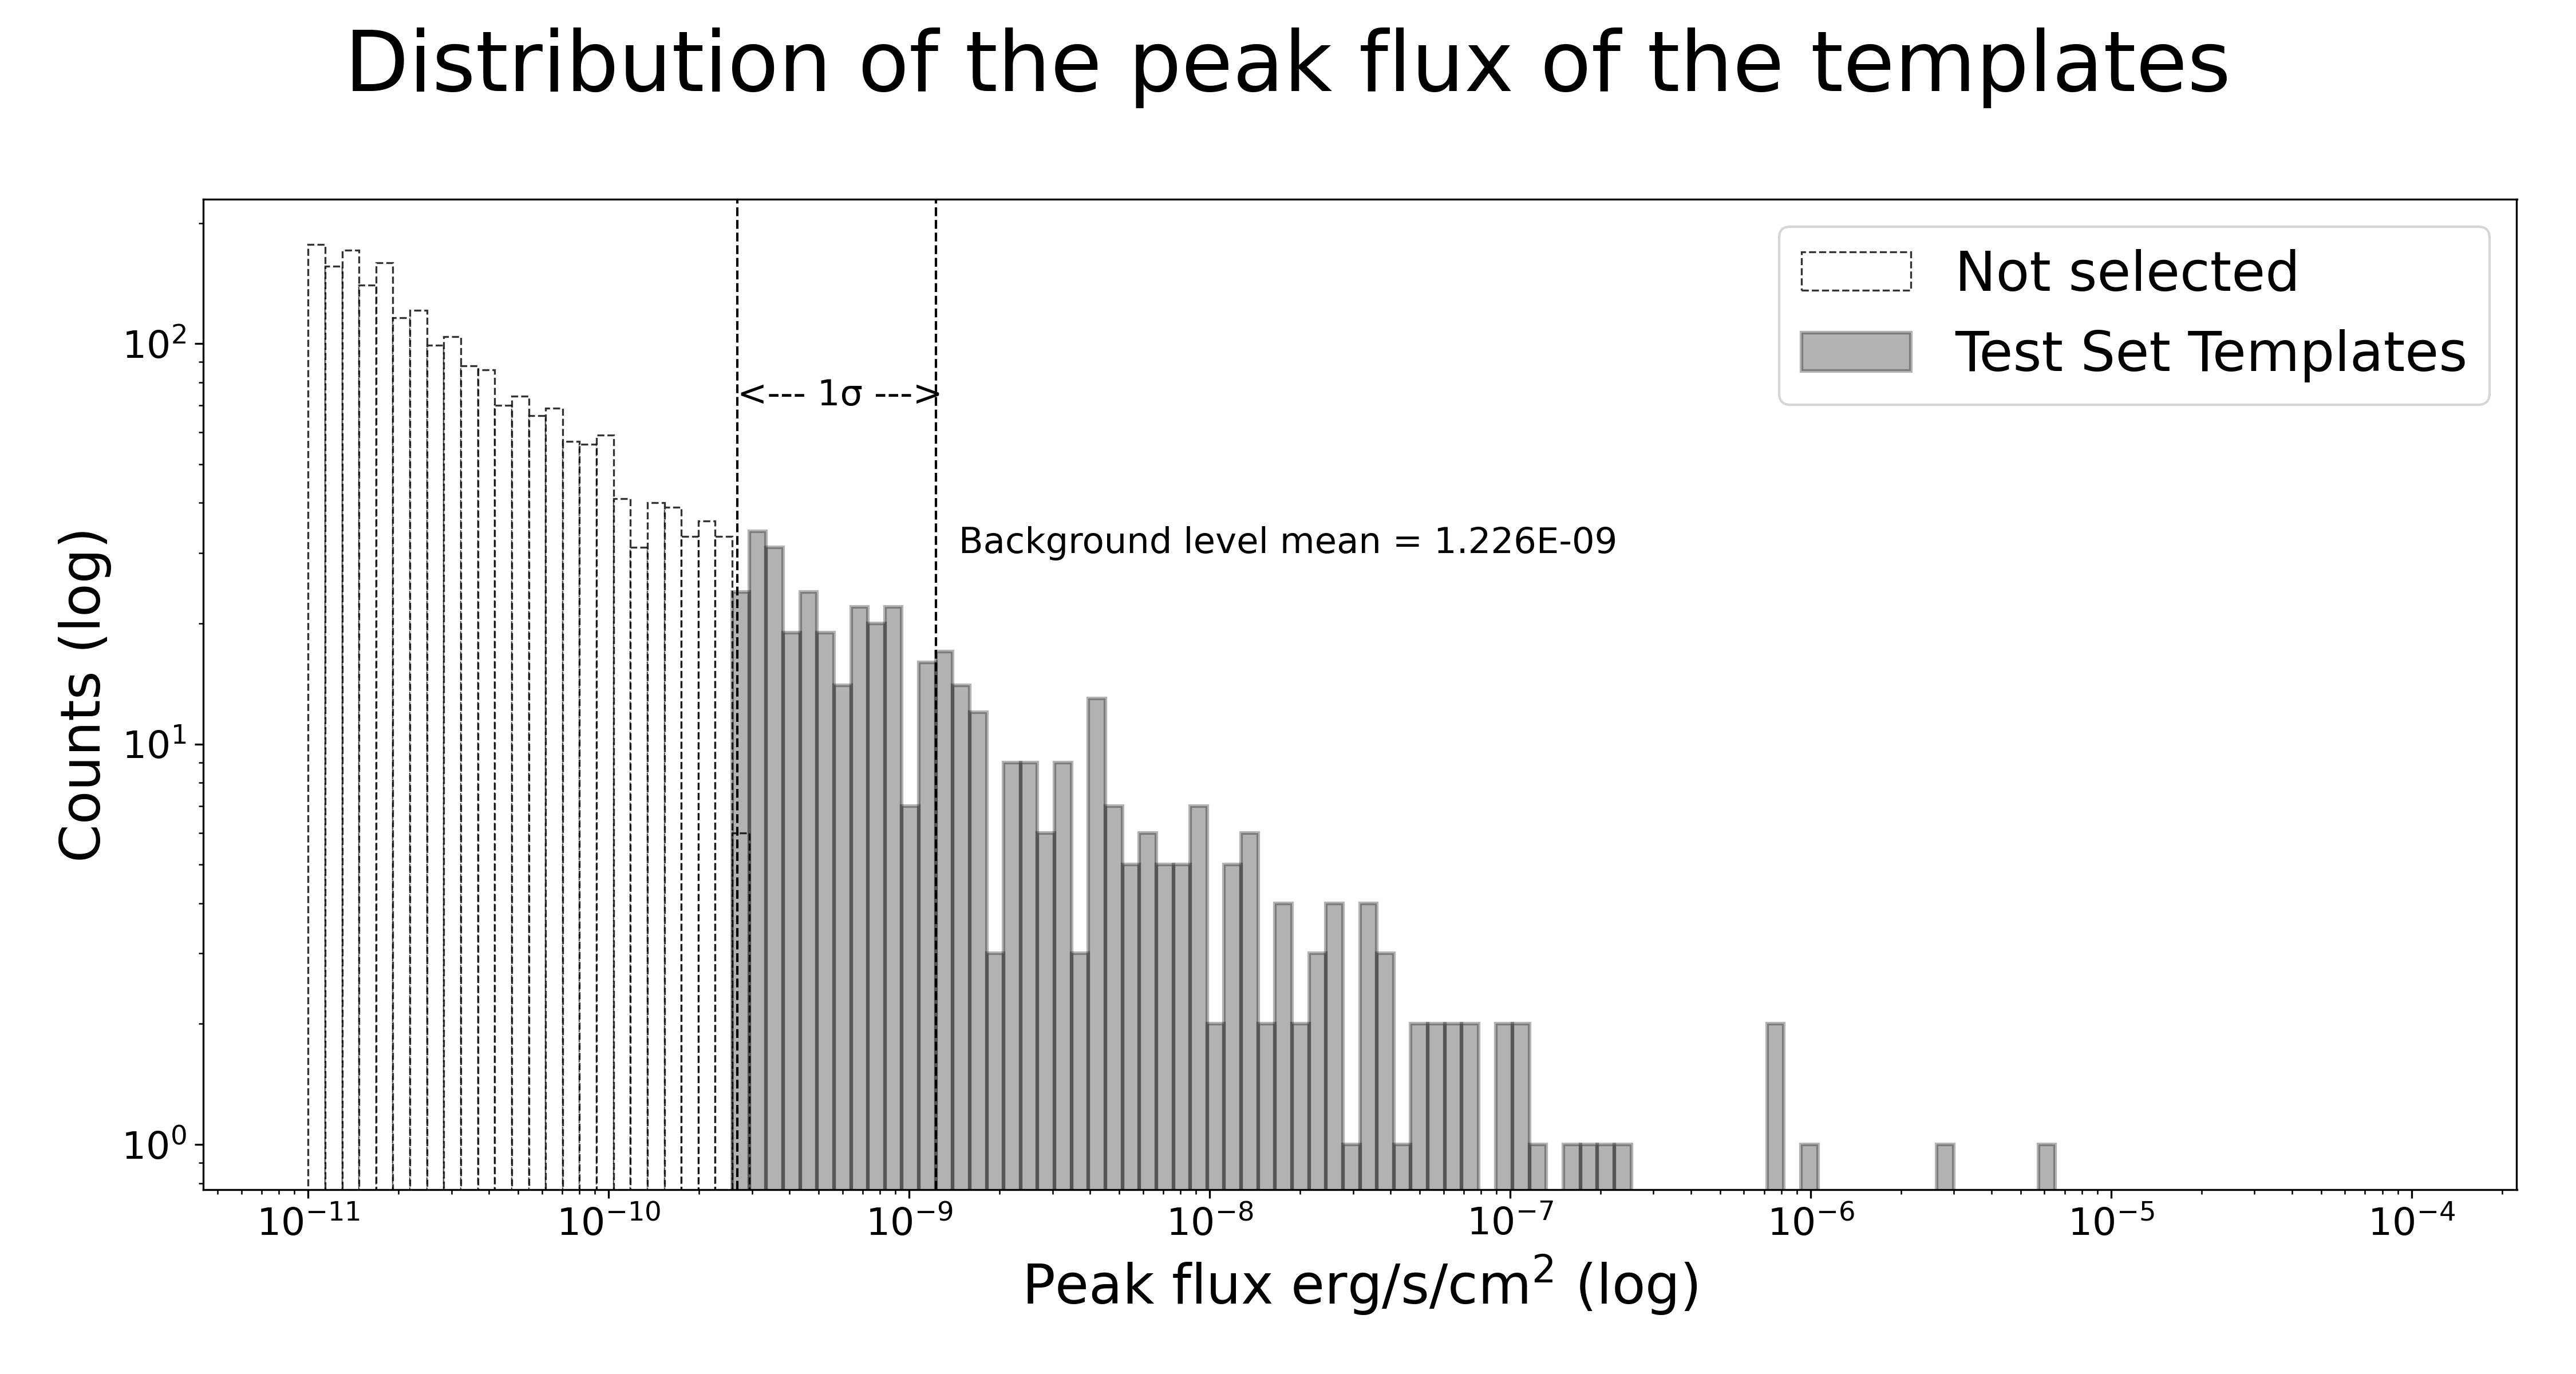
\includegraphics[width=1\textwidth]{figures/experiments/templates_max_flux_distributions.png}
\caption{The distribution of the maximum flux for each GRB template. The test sets E and H contain respectively 188  and 438 of GRB simulated trials, and their maximum fluxes are within: $[[1.2264e-09, \infty]]$ and $[[2.6785e-10, \infty]]$.}
\label{f:exp-max-flux-distribution-E}
\end{figure}


The simulation time is limited to 500 seconds because we are interested in the first part of the signal, given the nature of the scientific use cases described in Chapter [ref]. The trigger time that defines the GRB event's start is 250 seconds. The integration time is the same used for the training set generation for the reasons stated in \autoref{c:Contribution-2}. The autoencoder models have been trained with time series of lengths equal to 5, with each point being a flux measurement integrated in 5 seconds. Hence the same settings are used here. The stride parameter is set to 1 because this method can work with temporal bins that are statistically dependent, and this drastically reduces the time the model takes to wait for data during the online inference. Table [ref] summarizes the configuration parameters described above. A time series is labeled as anomalous if it contains at least one point of GRB signal. Figure [ref] shows some samples of GRB simulated trials.  

\subsection{P-value threshold and inference}
\label{s:P-Val-Inference}
Figures \ref{fig:ts-distribution-and-p-values-cnn-it-5}
\ref{fig:ts-distribution-and-p-values-rnn-it-5}
\ref{fig:ts-distribution-and-p-values-cnn-it-1}
\ref{fig:ts-distribution-and-p-values-rnn-it-1} show the distributions of the reconstruction errors and p-values for the A.D. CNN and RNN models and for integration times equal to 5 and 1. The following listing shows the thresholds the models use to issue detection with a $5\sigma$ significance. 
\begin{itemize}
    \item RNN model IT=5. Threshold: 0.00207 corresponding to $5.0488\sigma$.
    \item CNN model IT=5. Threshold: 0.0139 corresponding to $5.0465\sigma$.
    \item RNN model IT=1. Threshold: 0.0026 corresponding to $5.041\sigma$.
    \item CNN model IT=1. Threshold: 0.03164 corresponding to $5.0488\sigma$.
\end{itemize}

\begin{figure}
    \centering
    \subfigure{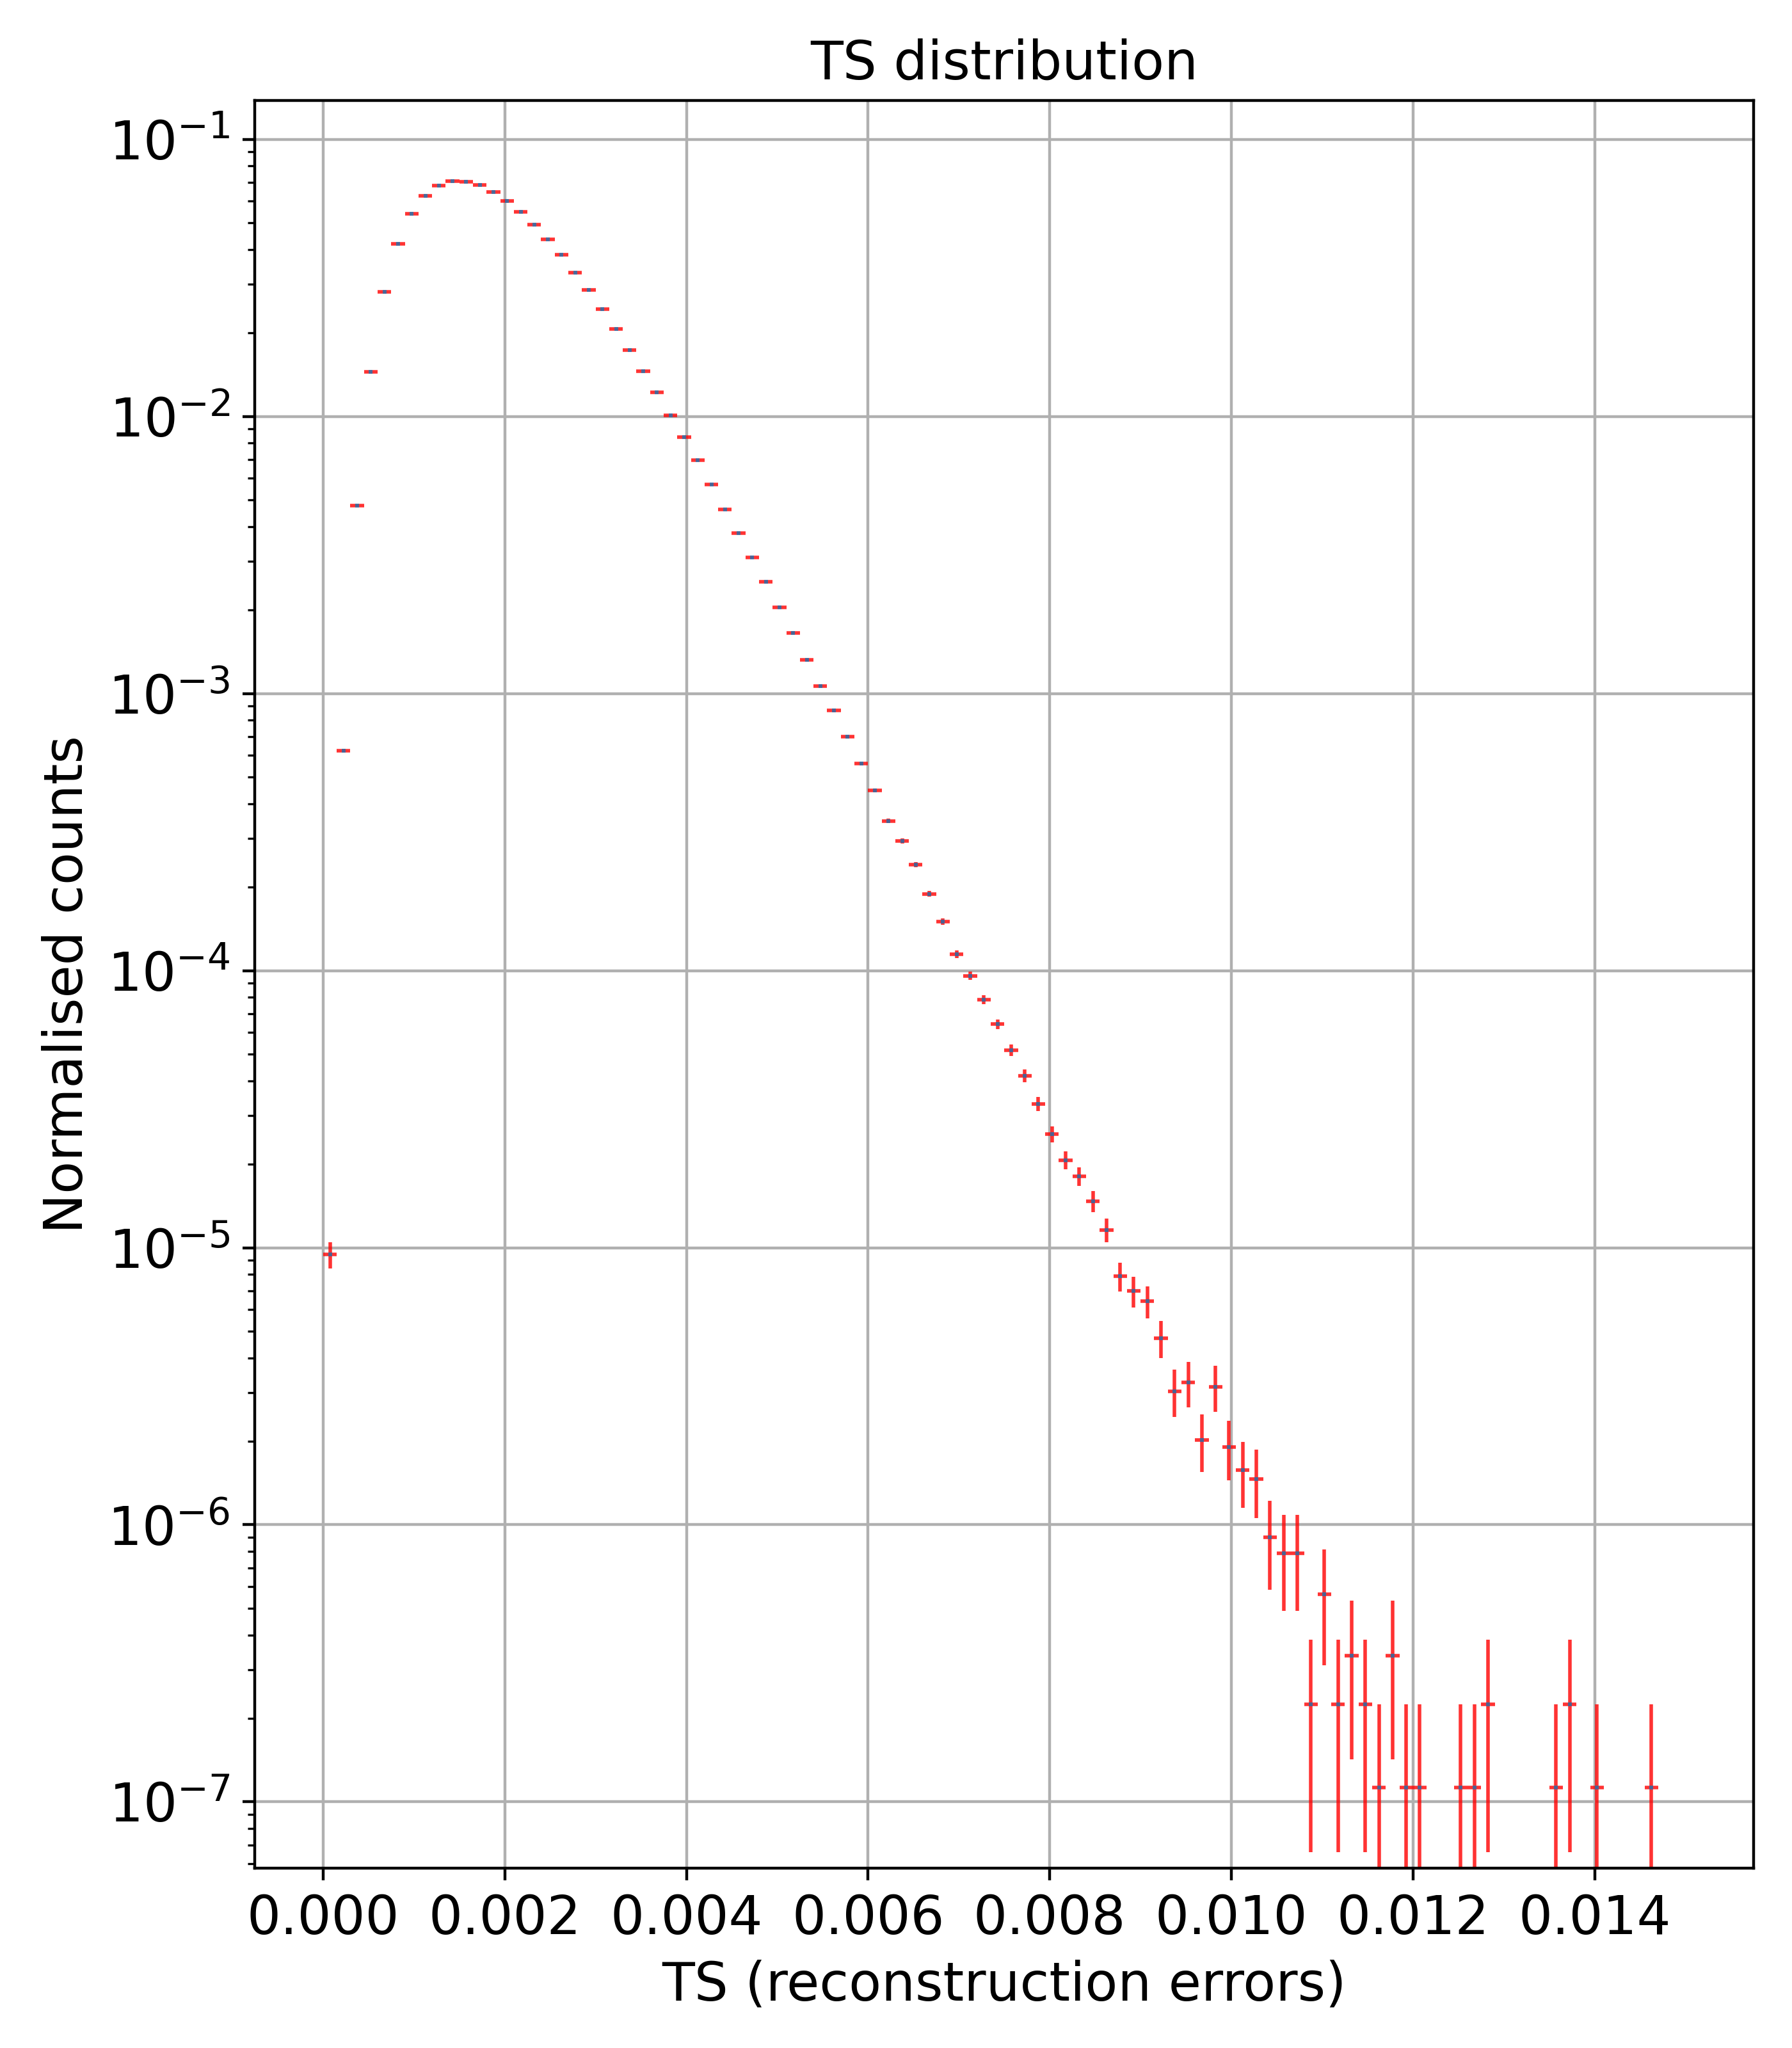
\includegraphics[width=0.5\textwidth]{figures/experiments/p_val/model_0/ts_distribution_bins_100.png}}
    
    \subfigure{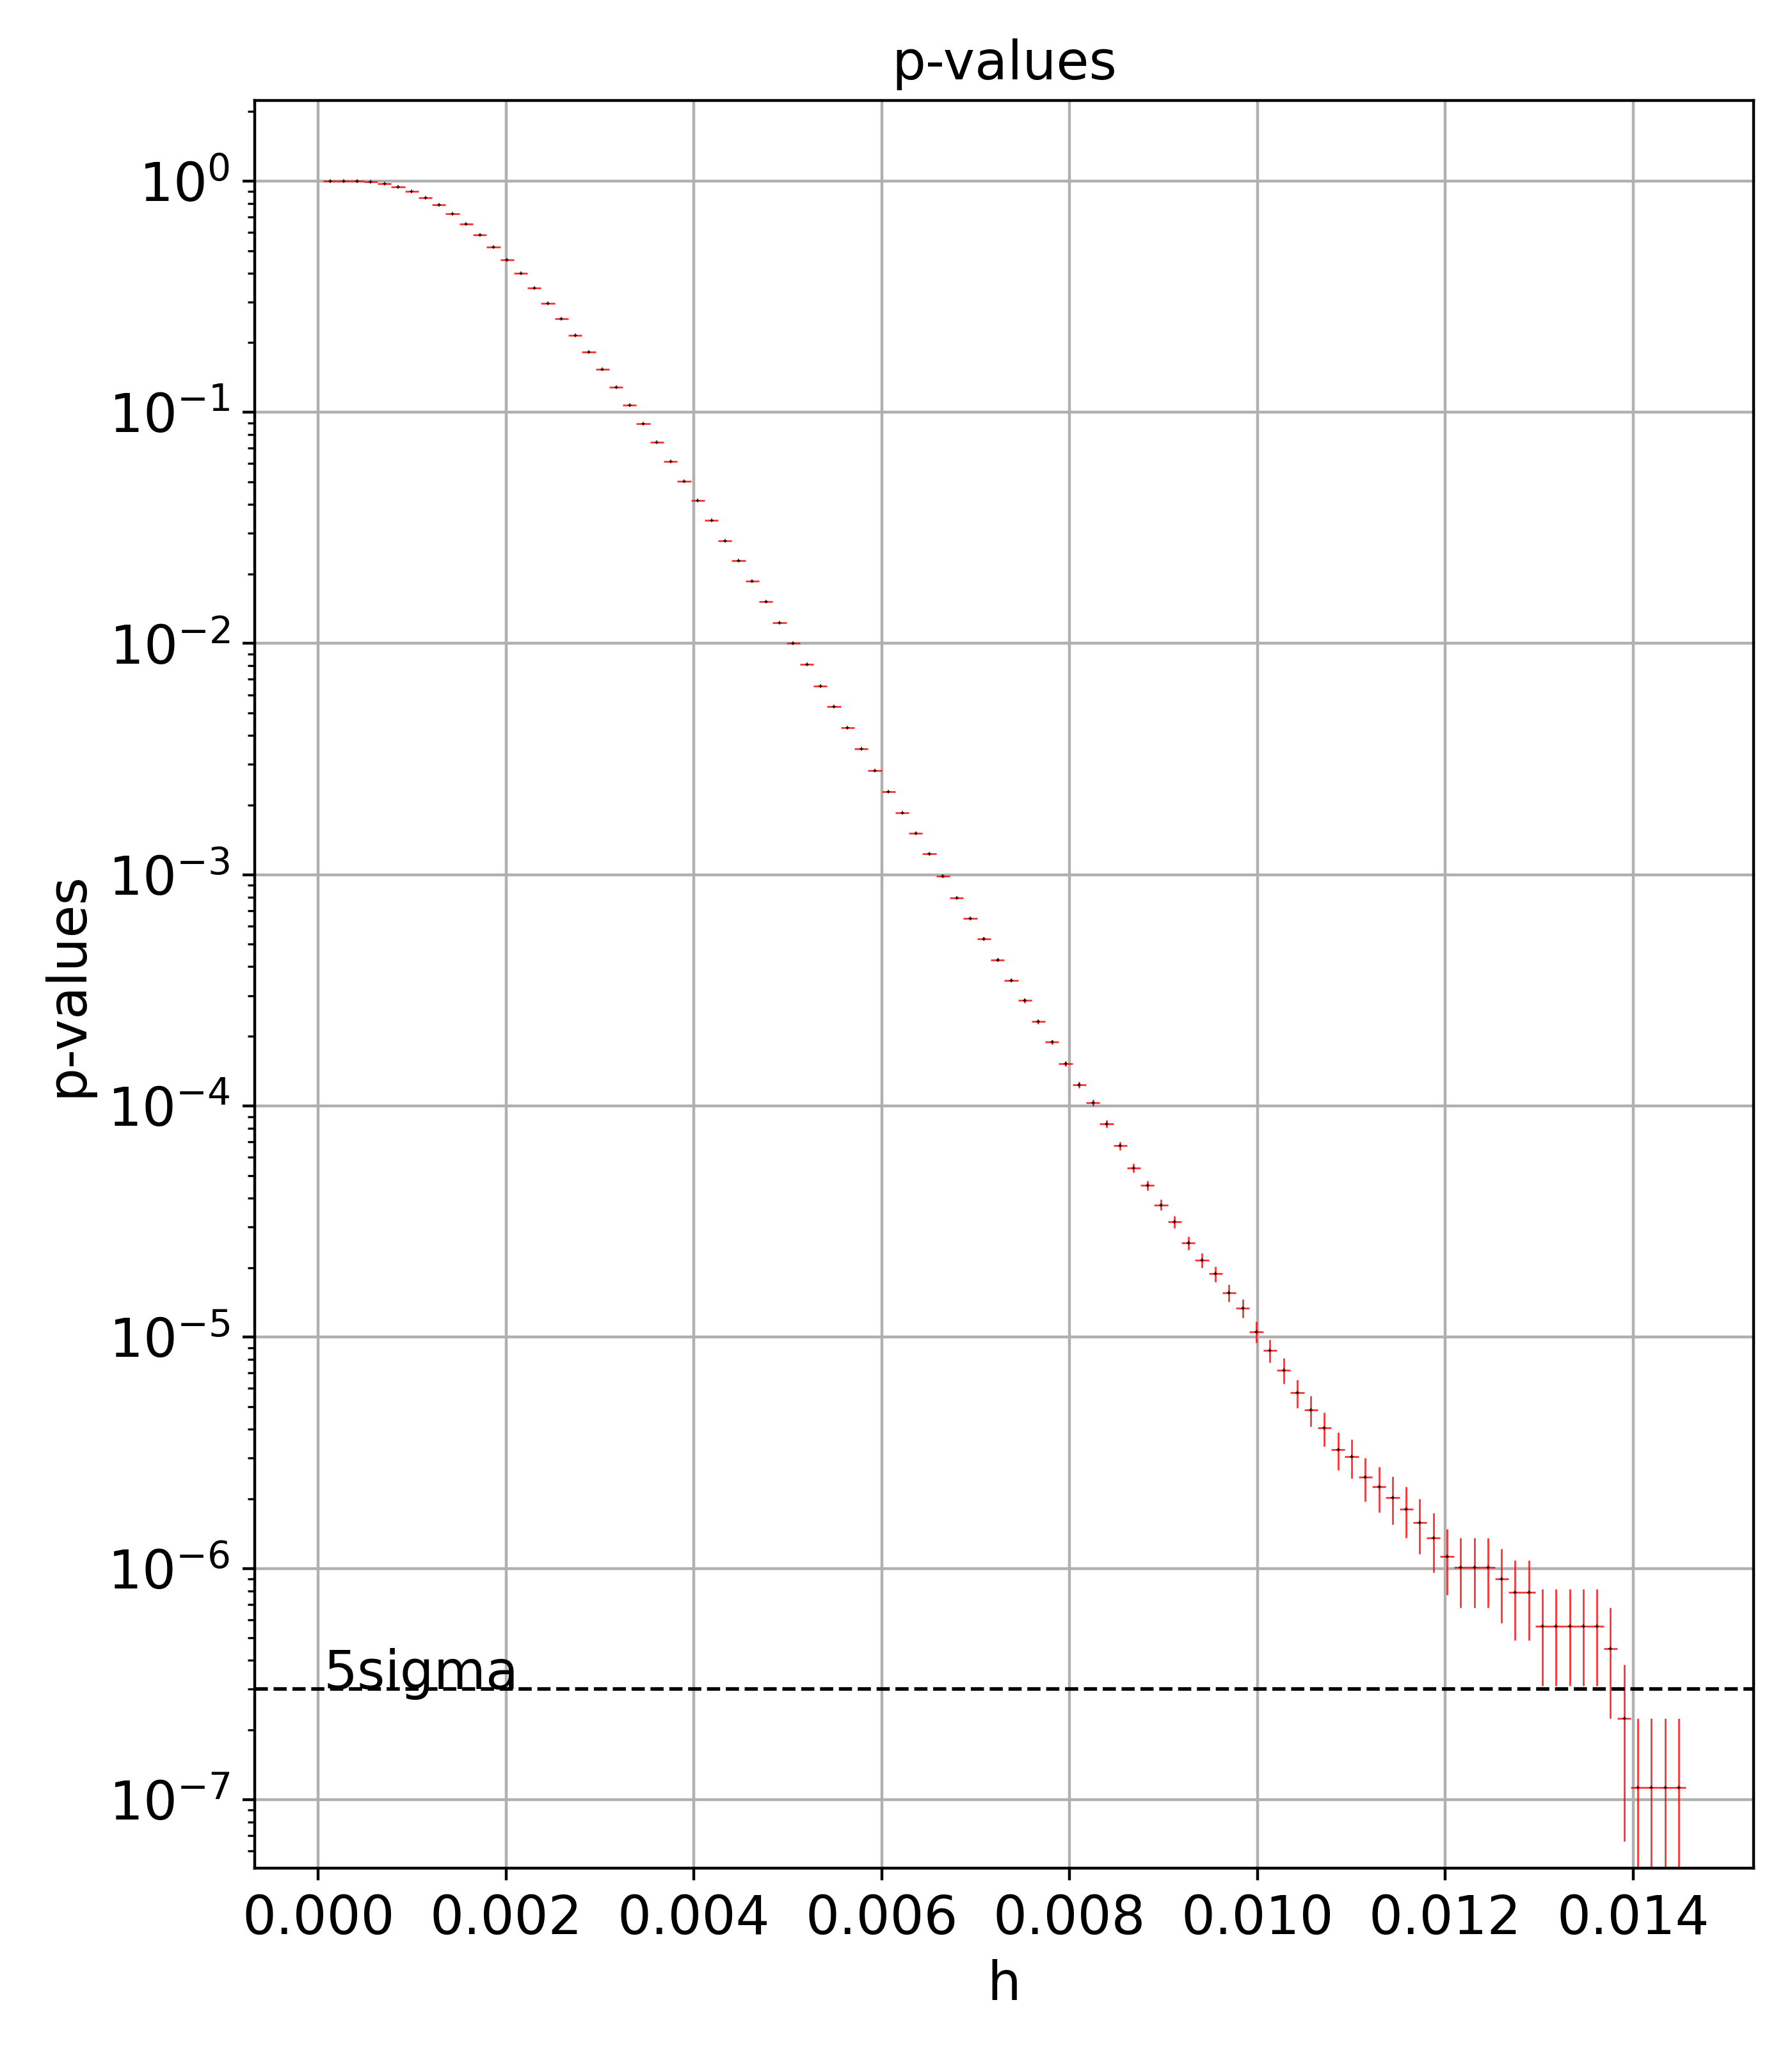
\includegraphics[width=0.5\textwidth]{figures/experiments/p_val/model_0/pvalue_bins_100.png}}
    
    \caption{TS distributions and p-values for A.D. cnn implementation for integration time = 5}
    \label{fig:ts-distribution-and-p-values-cnn-it-5}
\end{figure}

\begin{figure}
    \centering
    \subfigure{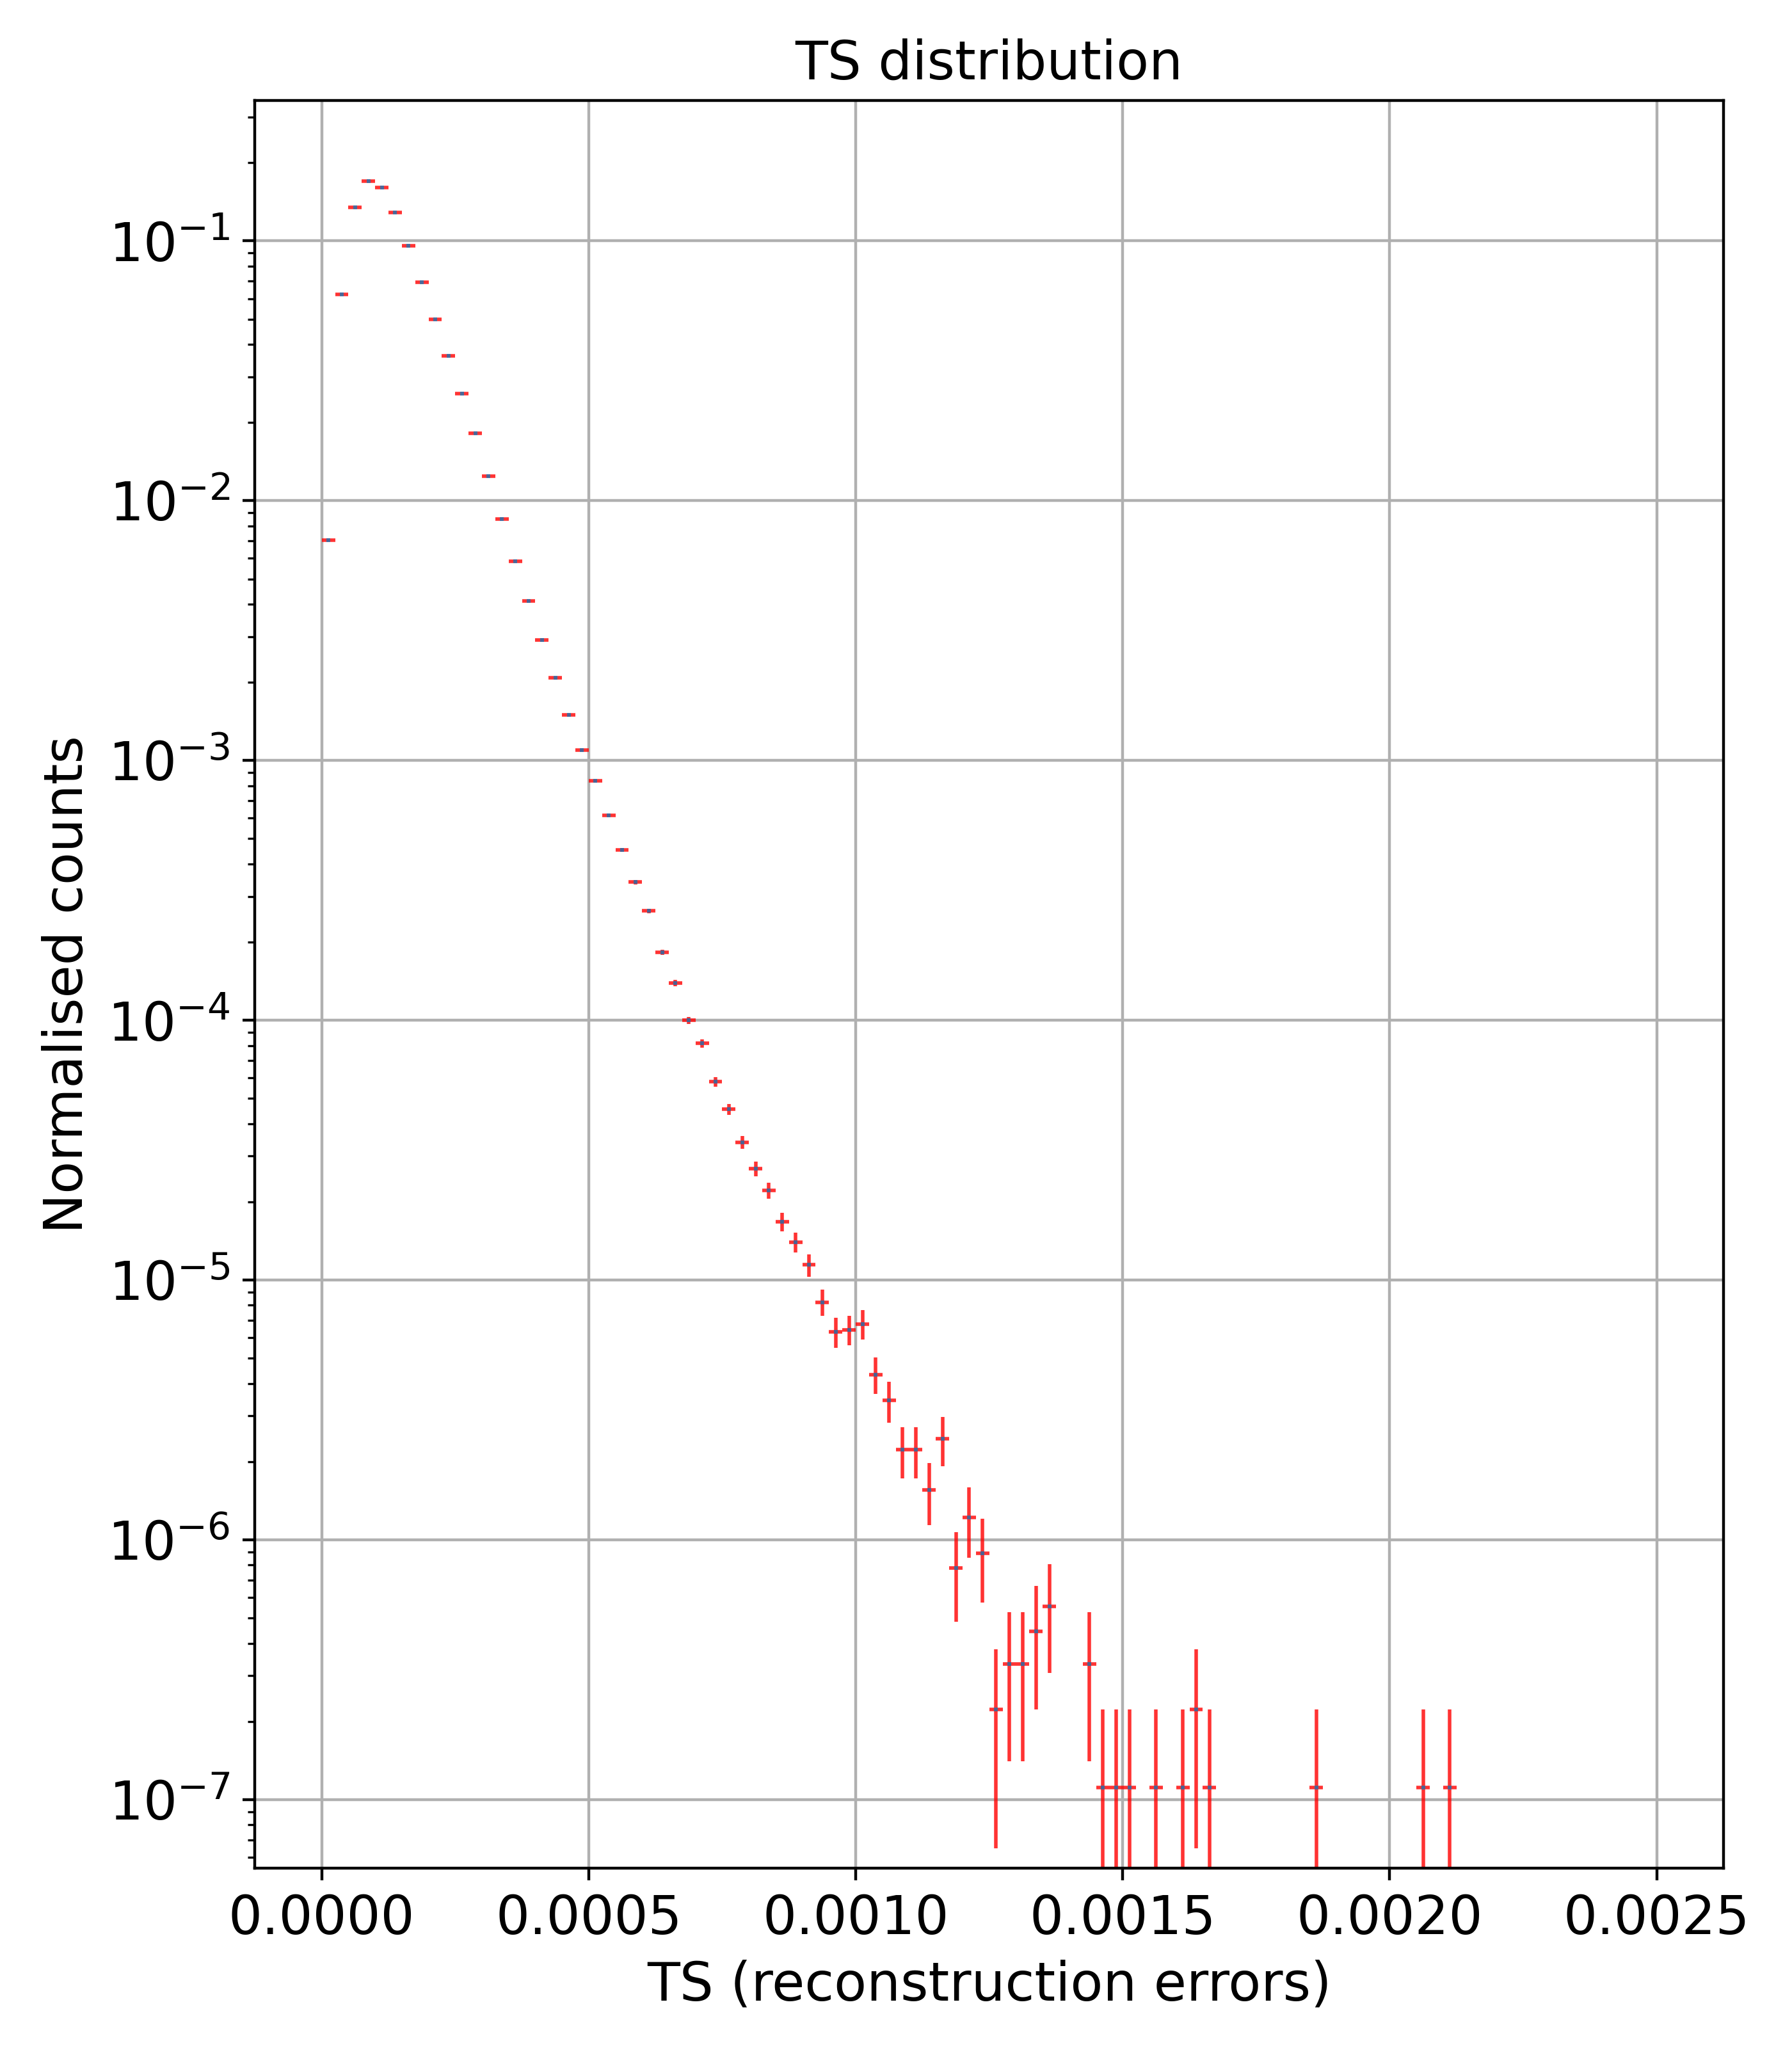
\includegraphics[width=0.5\textwidth]{figures/experiments/p_val/model_1/ts_distribution_bins_100.png}}
    
    \subfigure{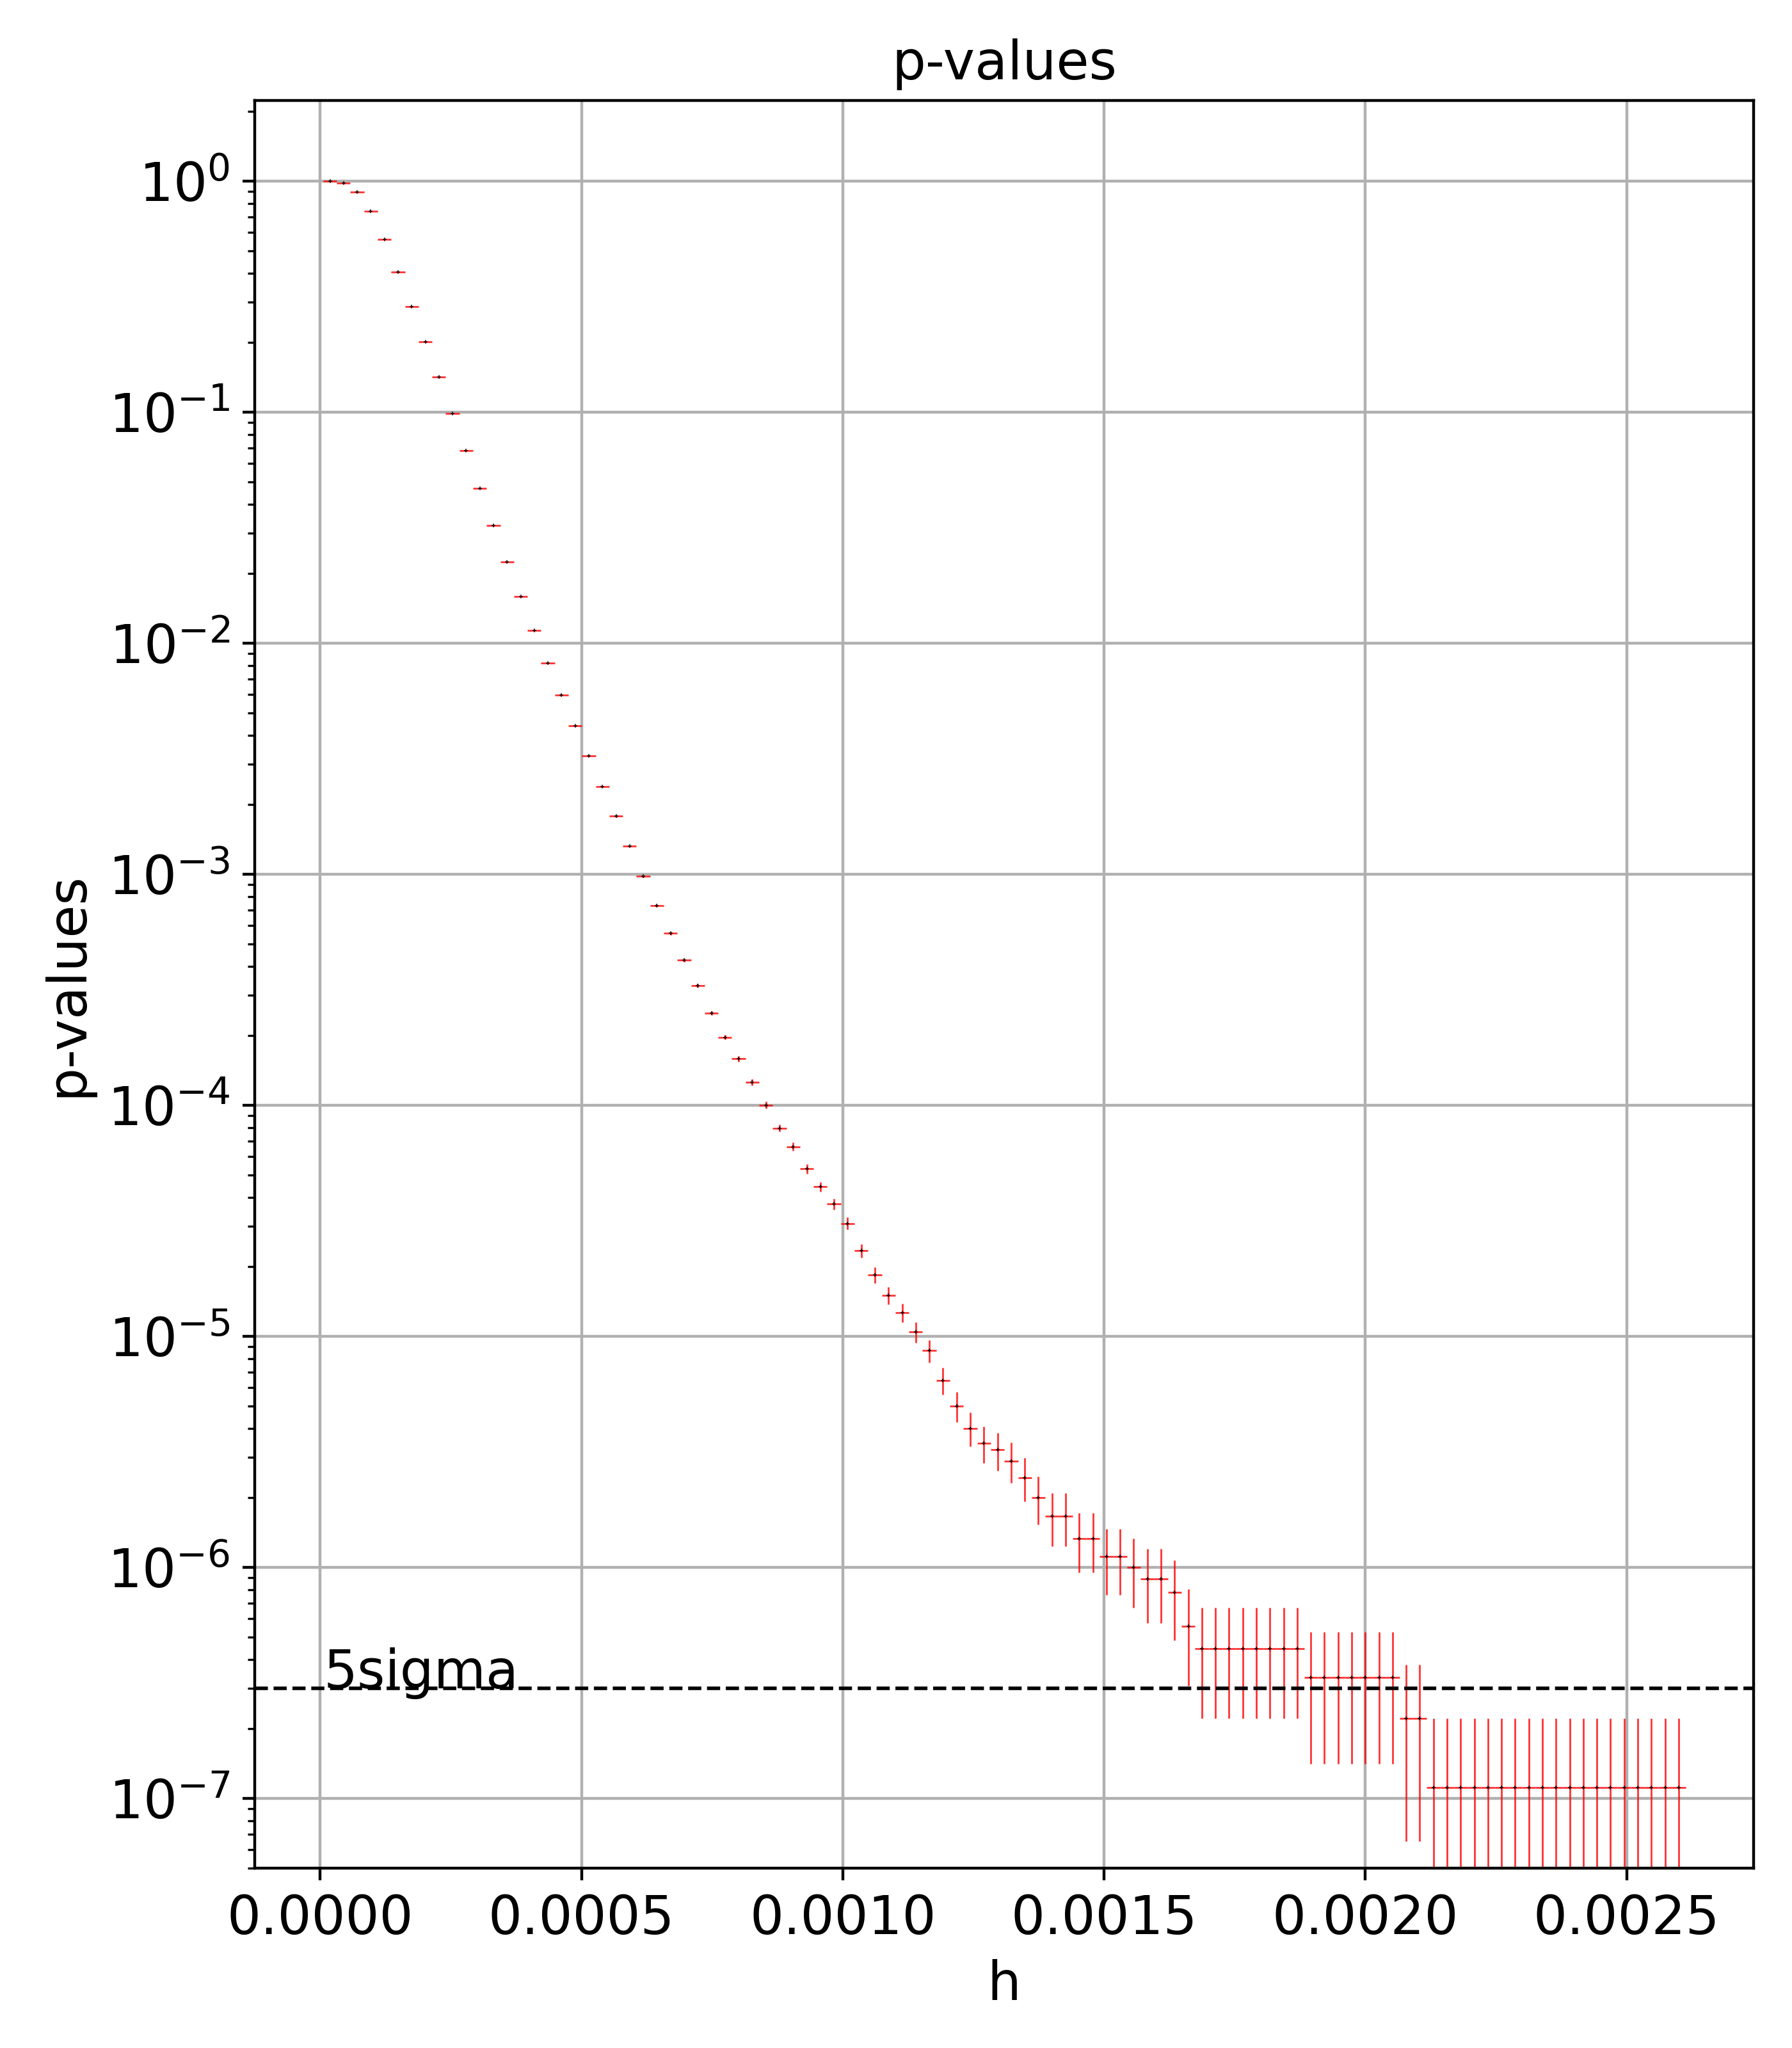
\includegraphics[width=0.5\textwidth]{figures/experiments/p_val/model_1/pvalue_bins_100.png}}
    
    \caption{TS distributions and p-values for A.D. rnn implementation for integration time = 5}
    \label{fig:ts-distribution-and-p-values-rnn-it-5}
\end{figure}


\begin{figure}
    \centering
    \subfigure{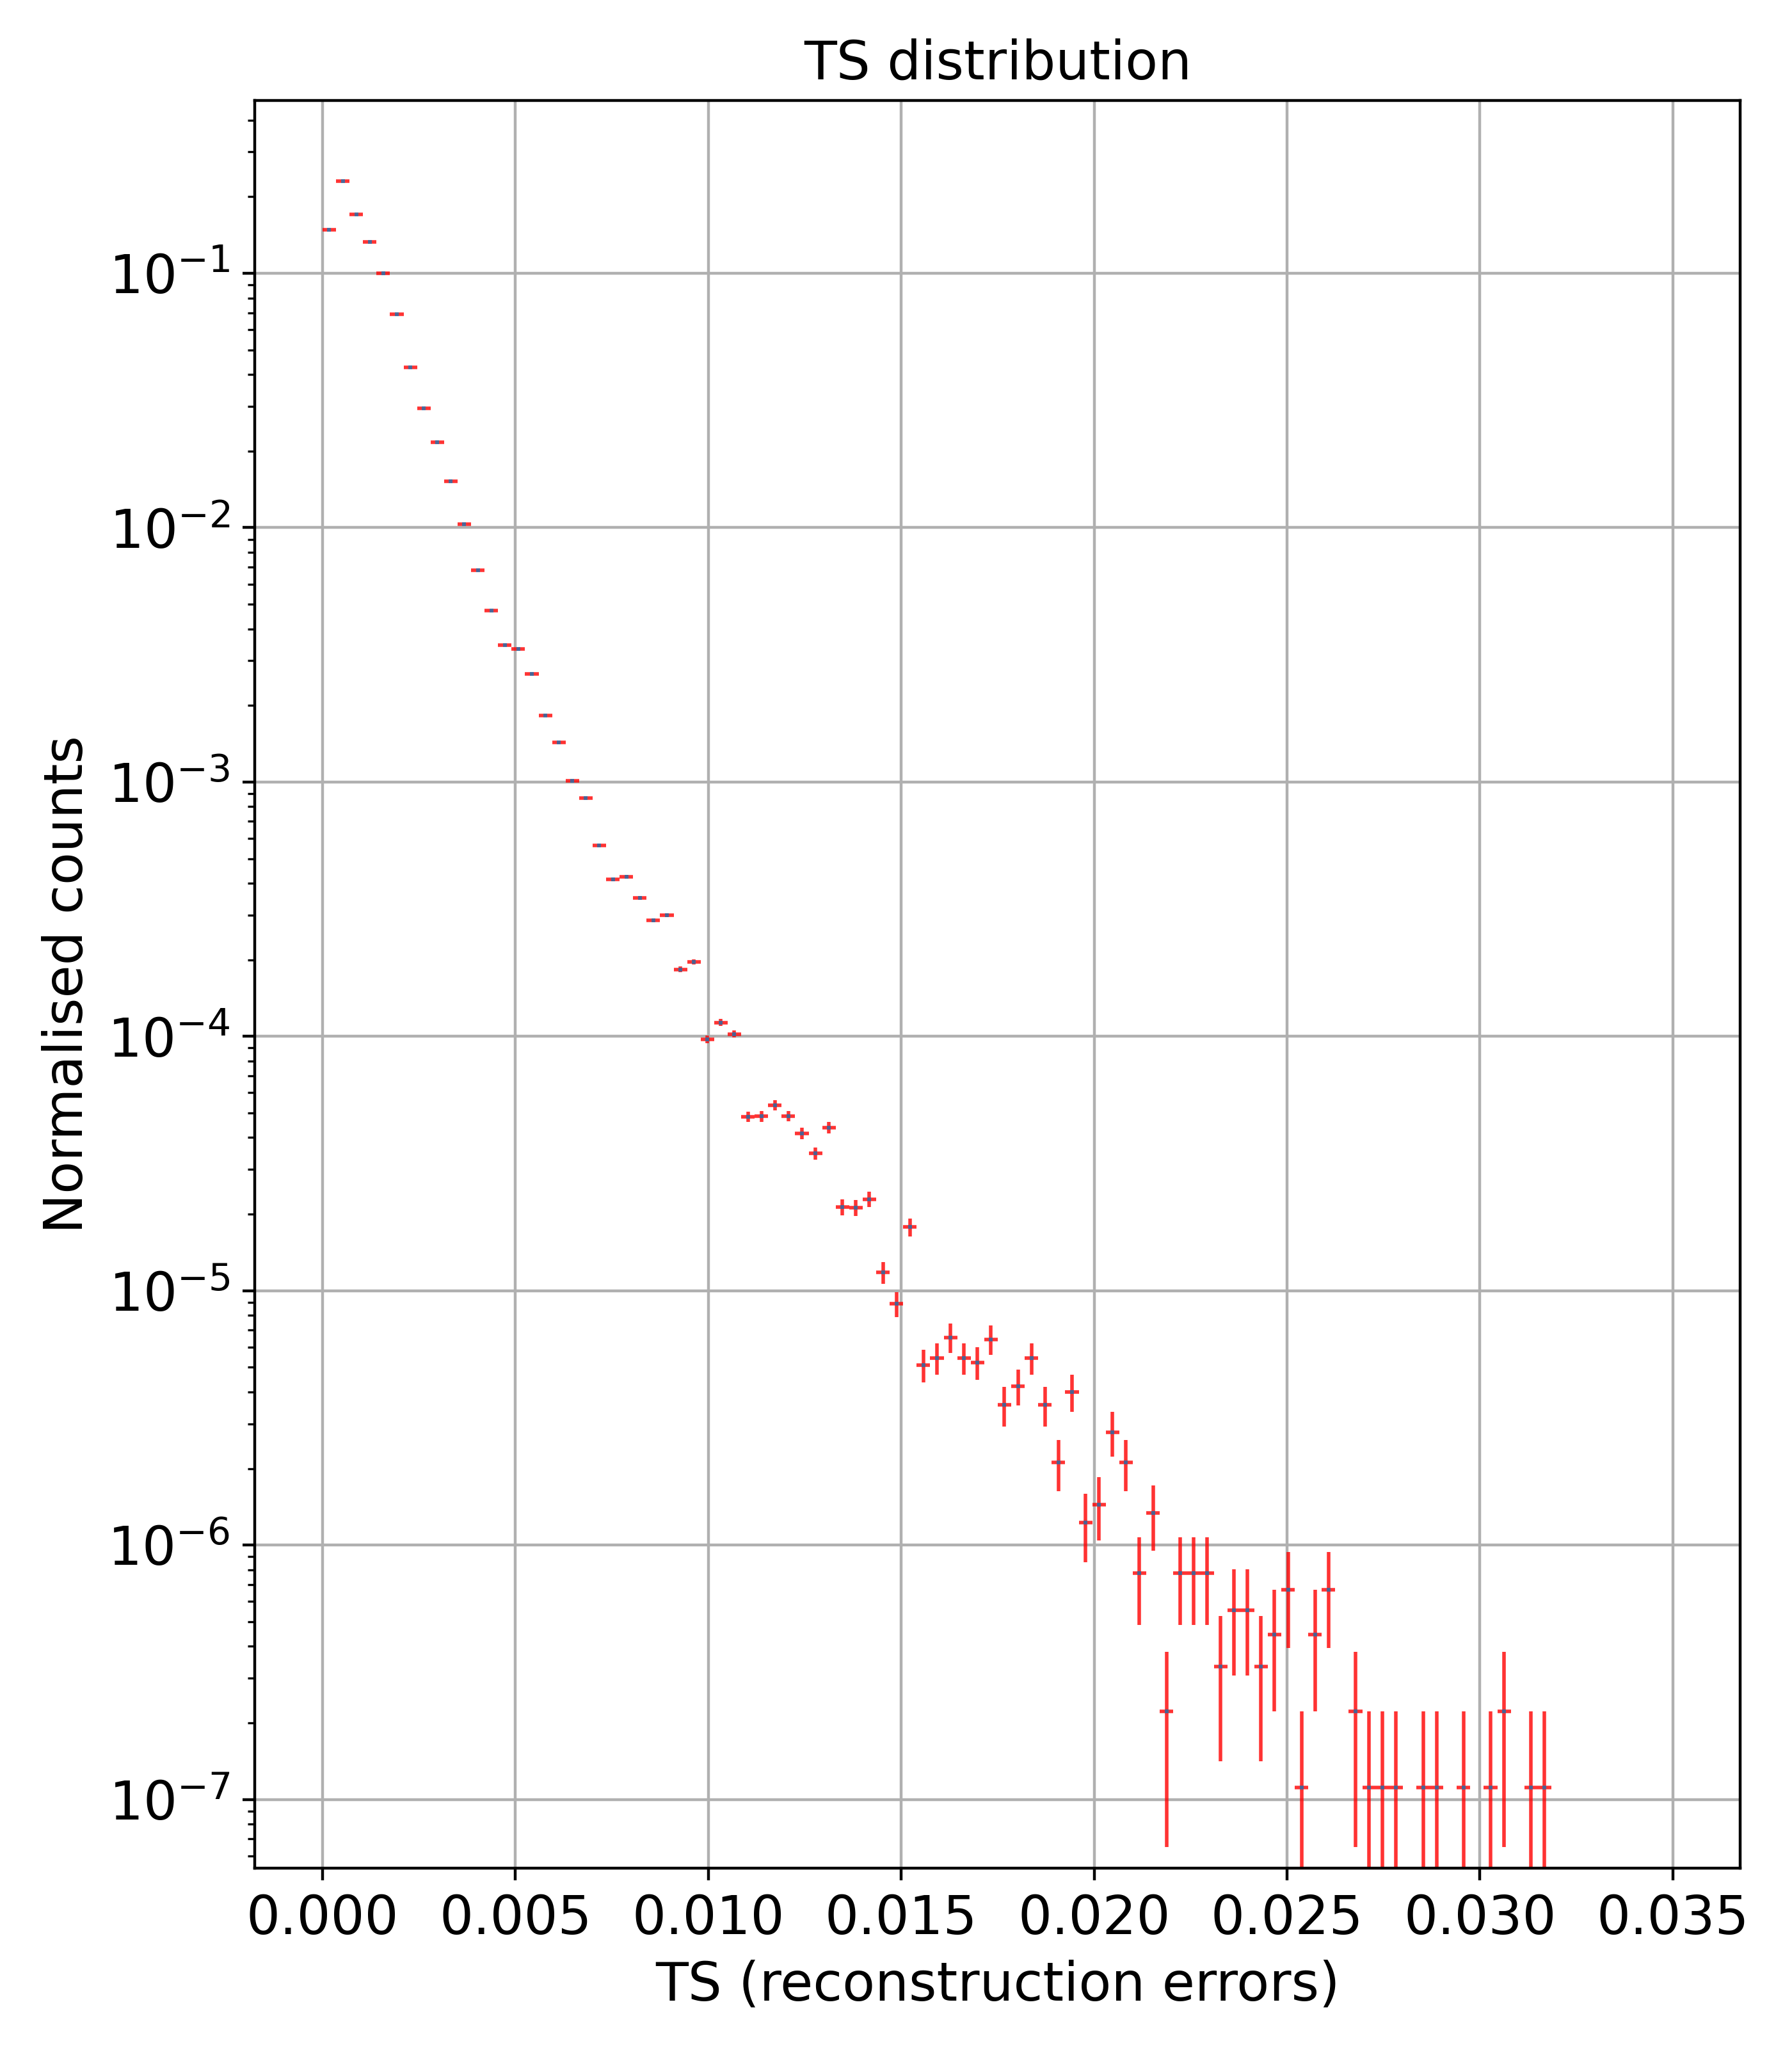
\includegraphics[width=0.5\textwidth]{figures/experiments/p_val/model_6/ts_distribution_bins_100.png}}
    
    \subfigure{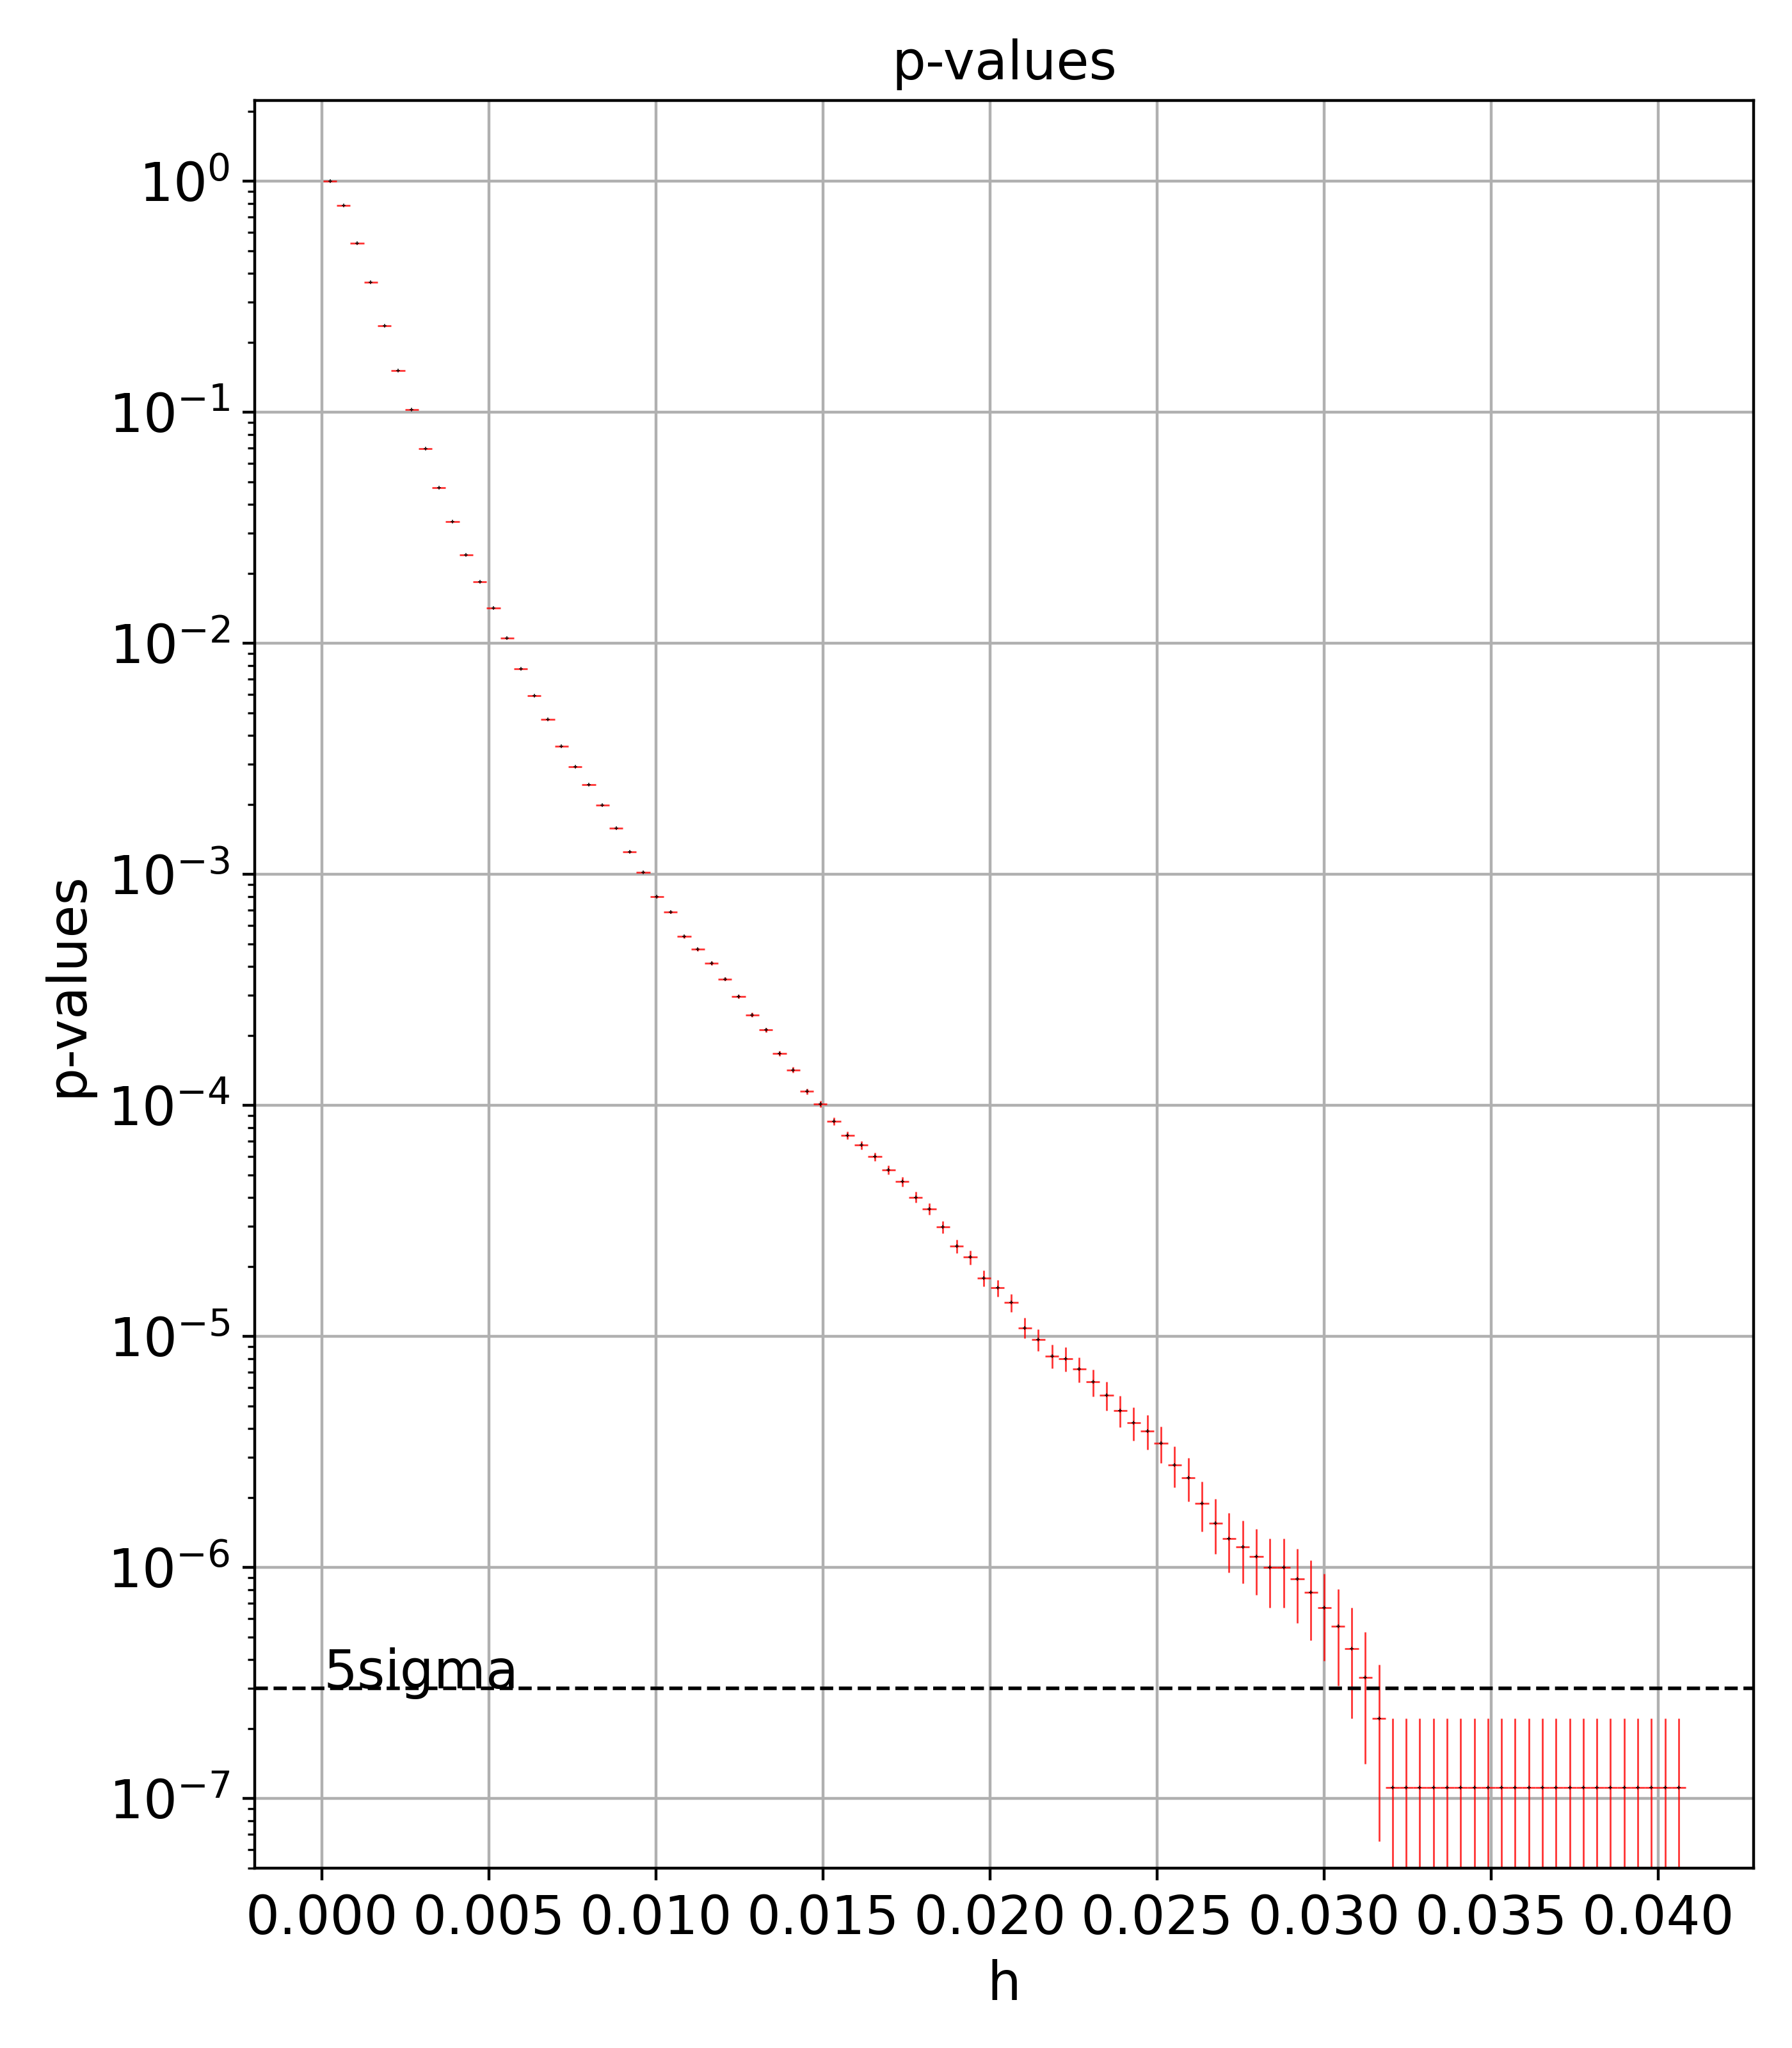
\includegraphics[width=0.5\textwidth]{figures/experiments/p_val/model_6/pvalue_bins_100.png}}
    
    \caption{TS distributions and p-values for A.D. cnn implementation for integration time = 5}
    \label{fig:ts-distribution-and-p-values-cnn-it-5}
\end{figure}

\begin{figure}
    \centering
\subfigure{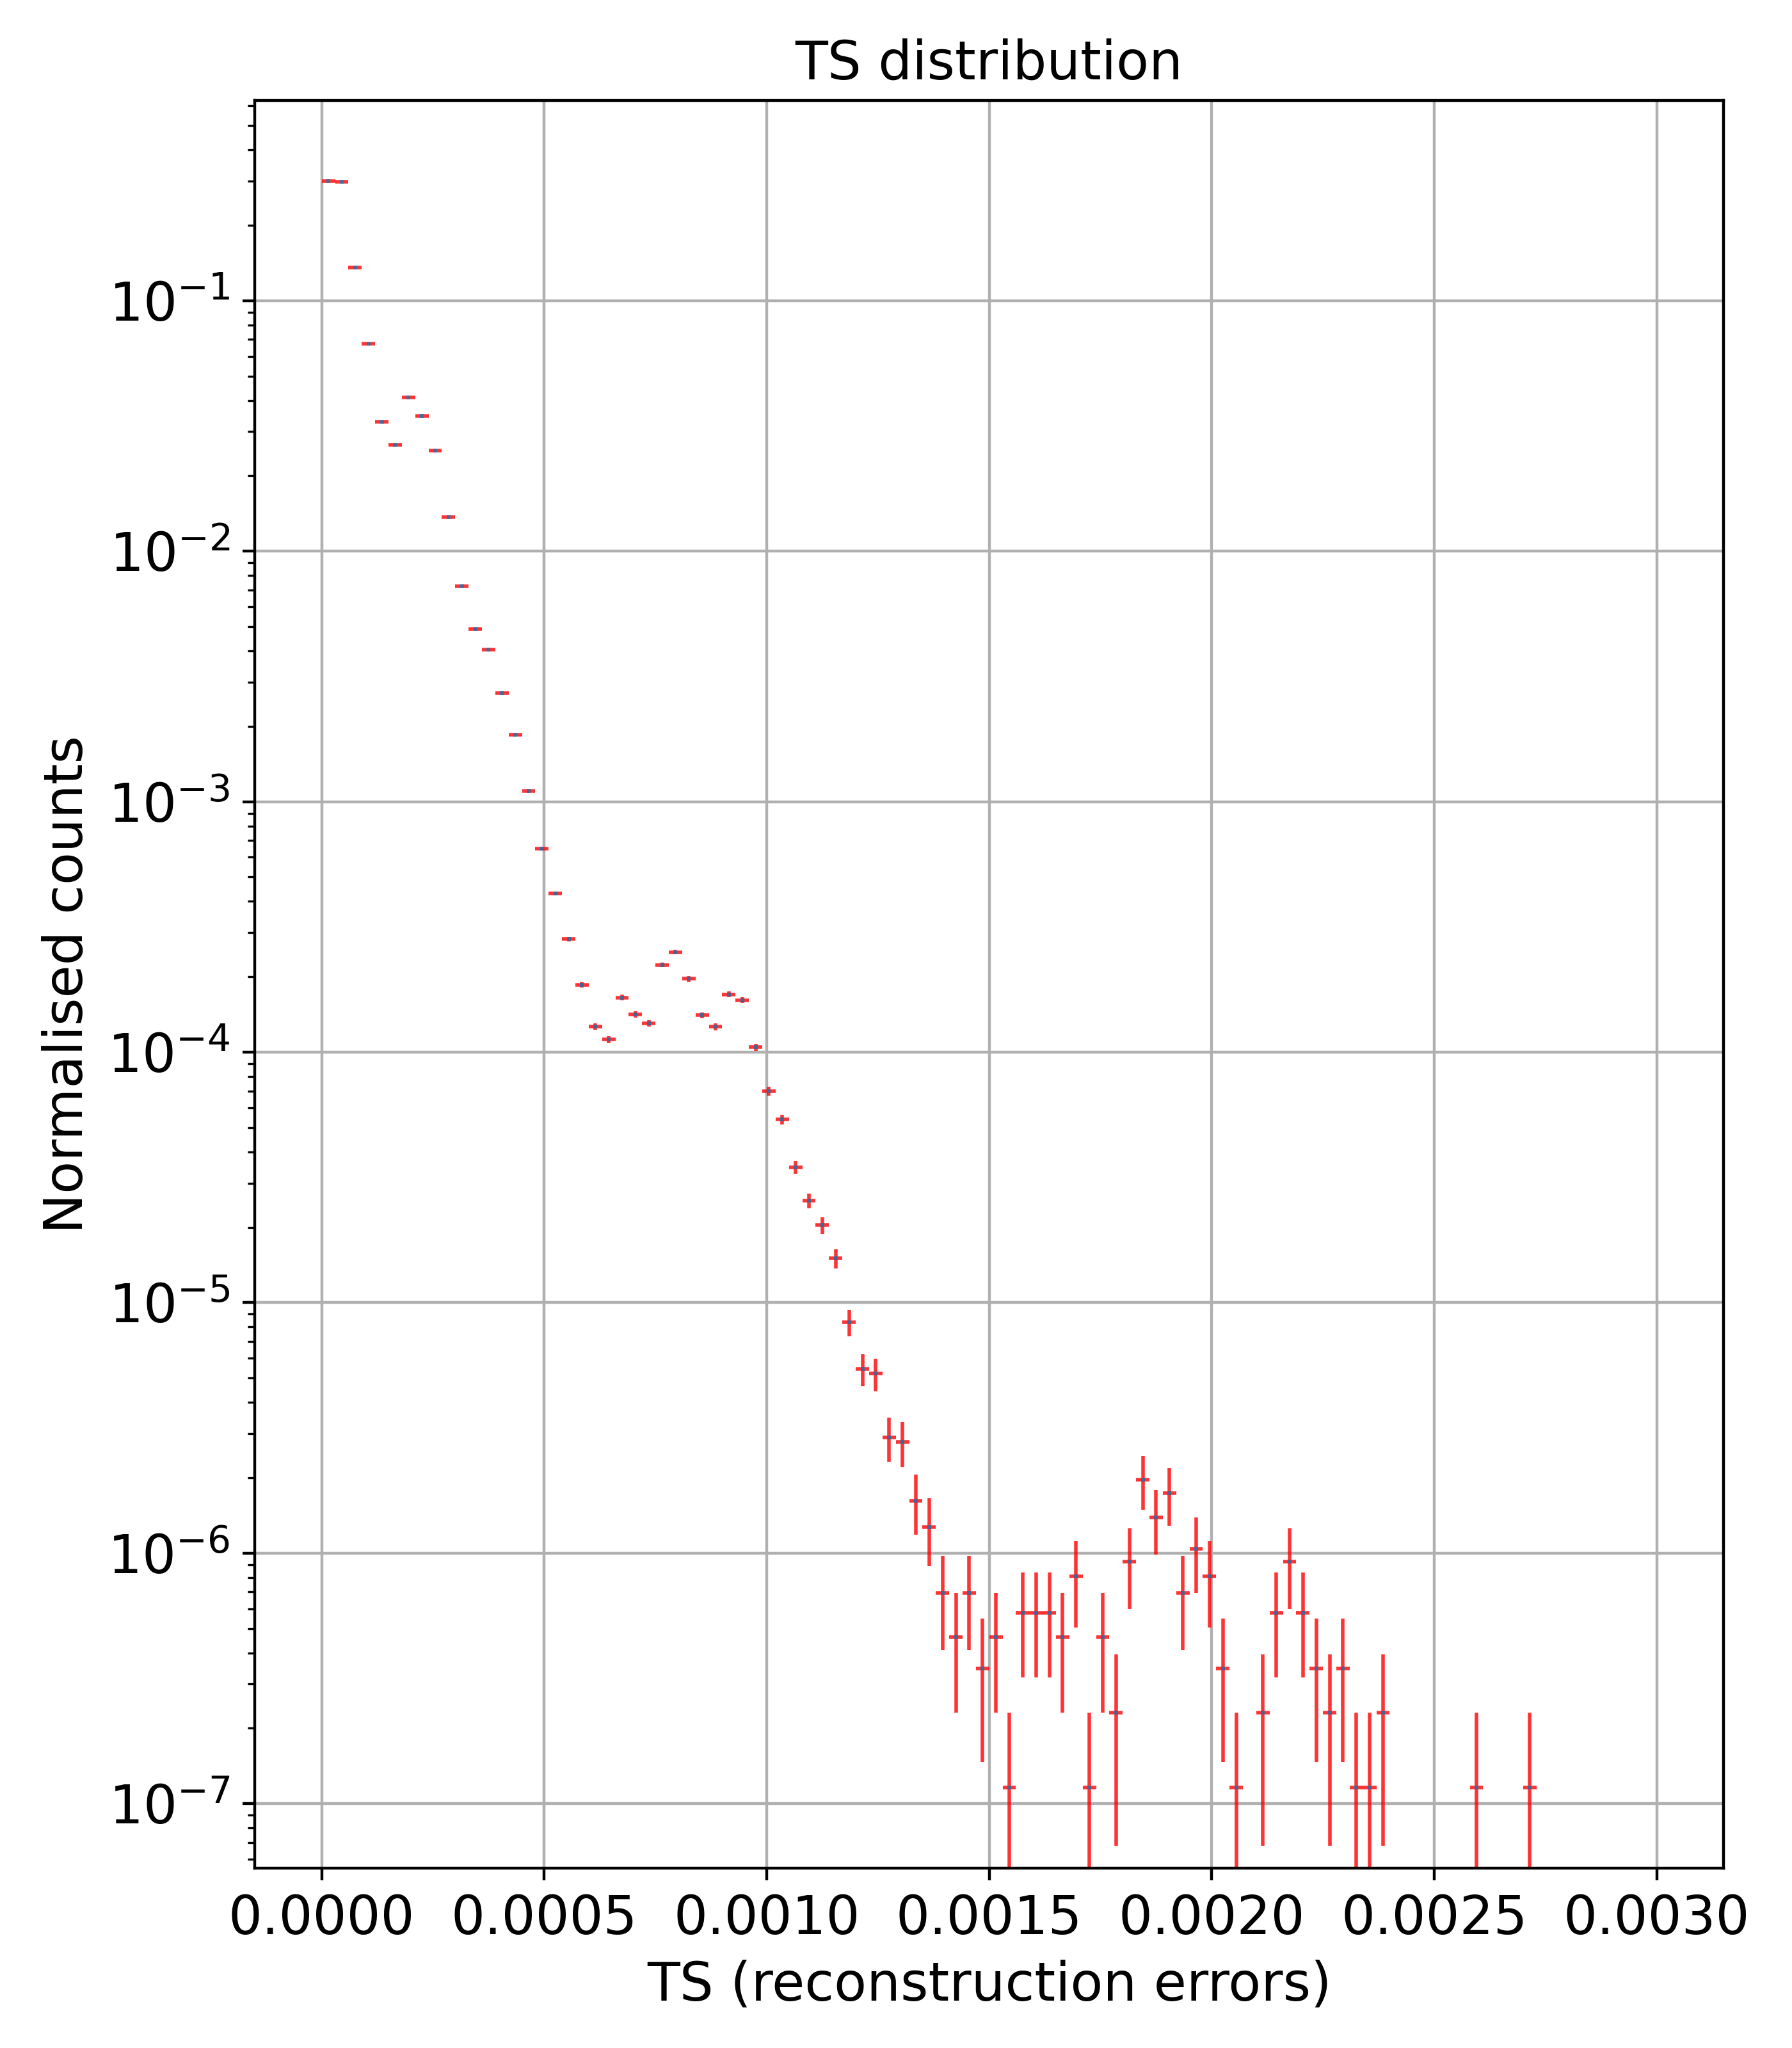
\includegraphics[width=0.5\textwidth]{figures/experiments/p_val/model_7/ts_distribution_bins_100.png}}
    \subfigure{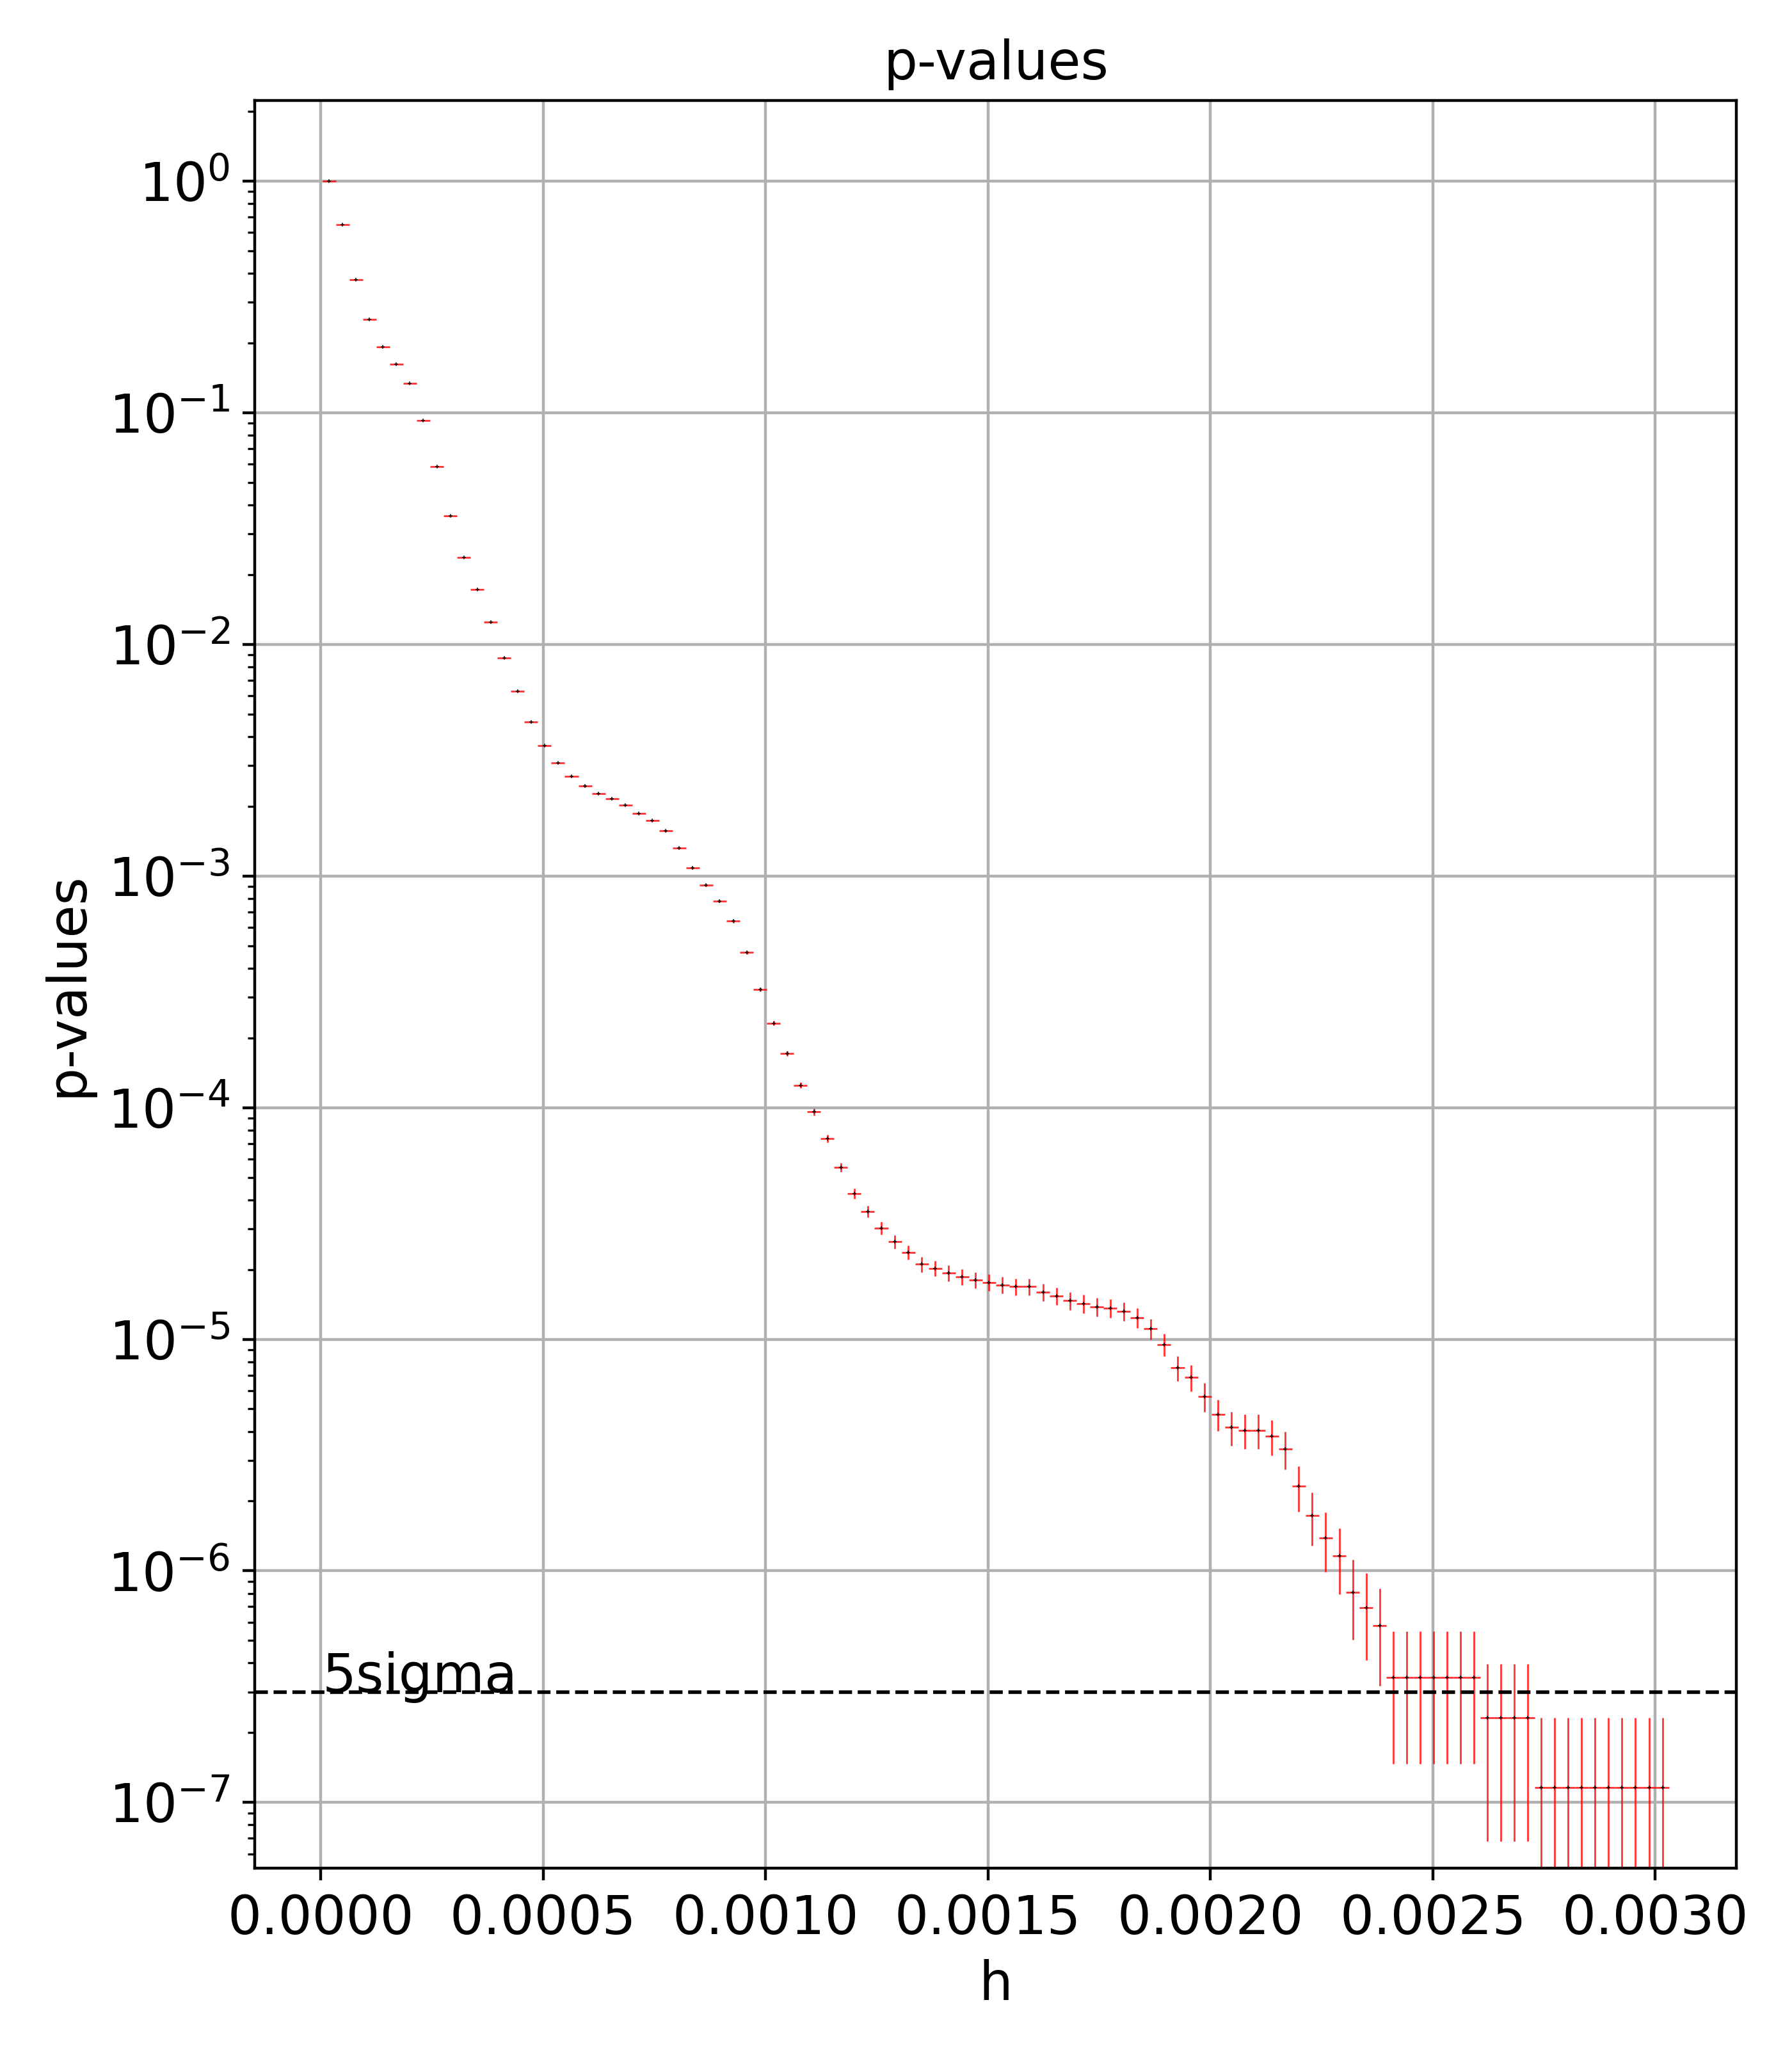
\includegraphics[width=0.5\textwidth]{figures/experiments/p_val/model_7/pvalue_bins_100.png}}
    
    \caption{TS distributions and p-values for A.D. rnn implementation for integration time = 1}
    \label{fig:ts-distribution-and-p-values-rnn-it-1}
\end{figure}

\begin{figure}
    \centering
    \subfigure{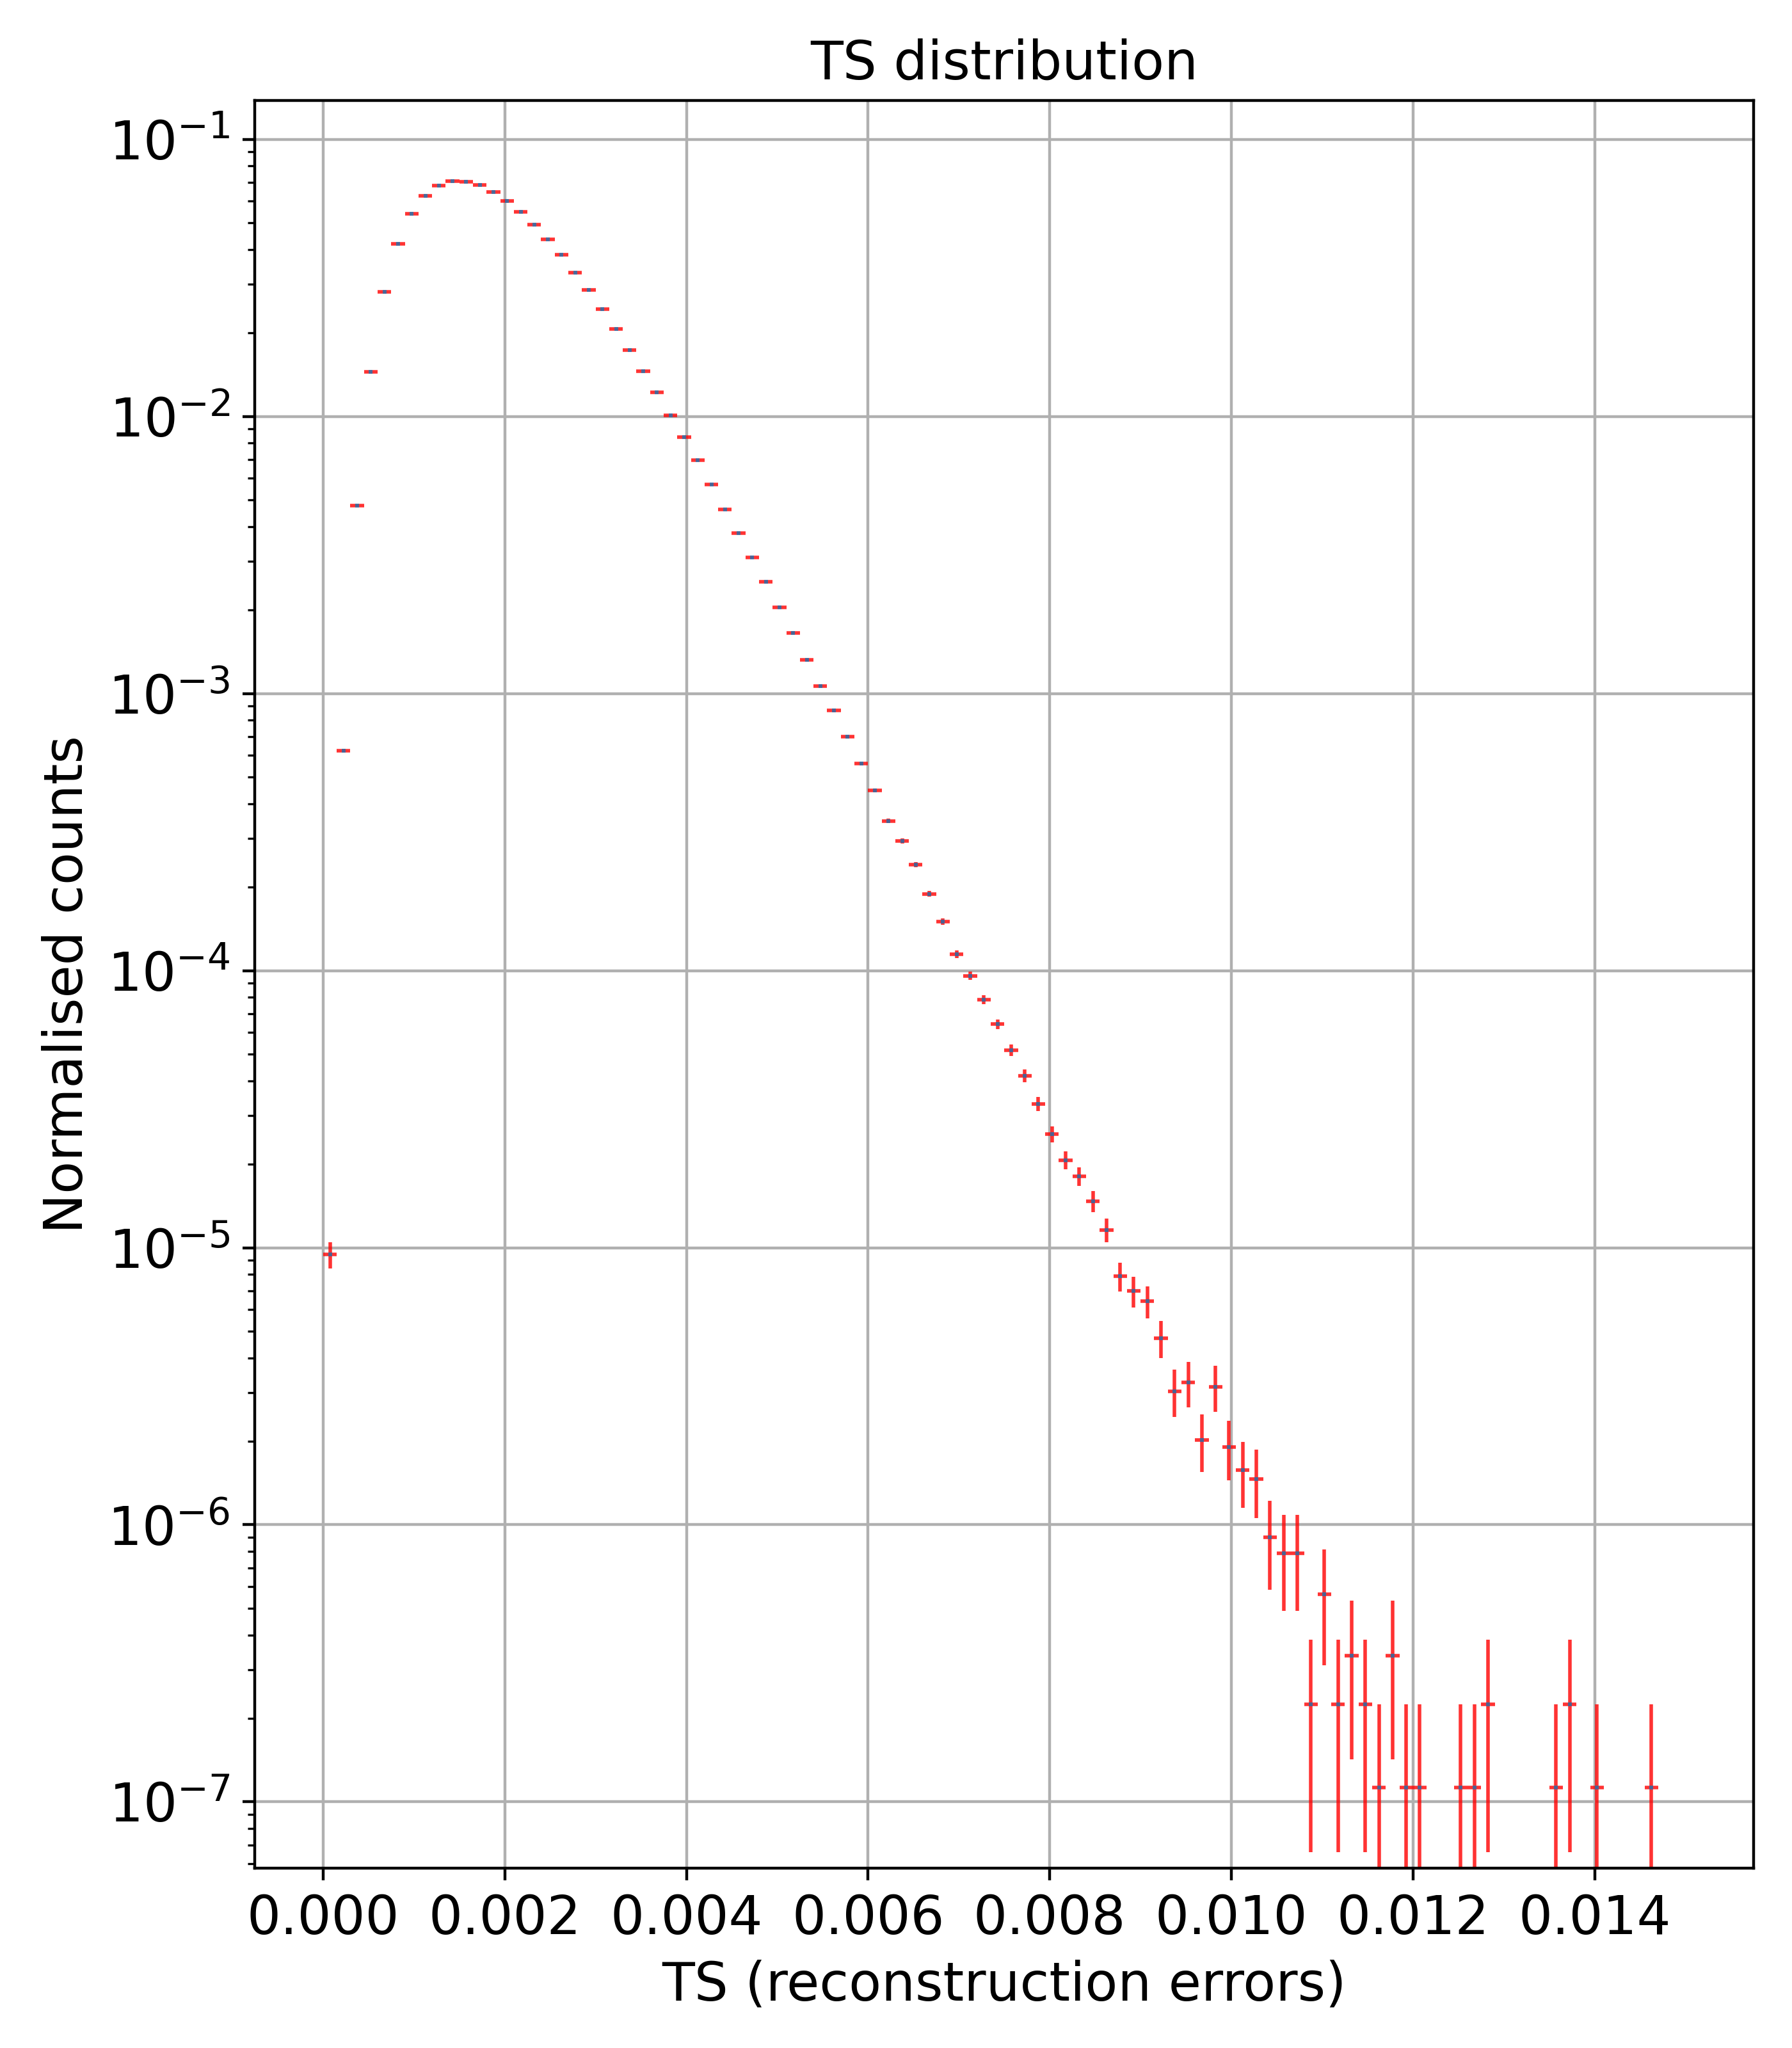
\includegraphics[width=0.5\textwidth]{figures/experiments/p_val/model_0/ts_distribution_bins_100.png}}
    
    \subfigure{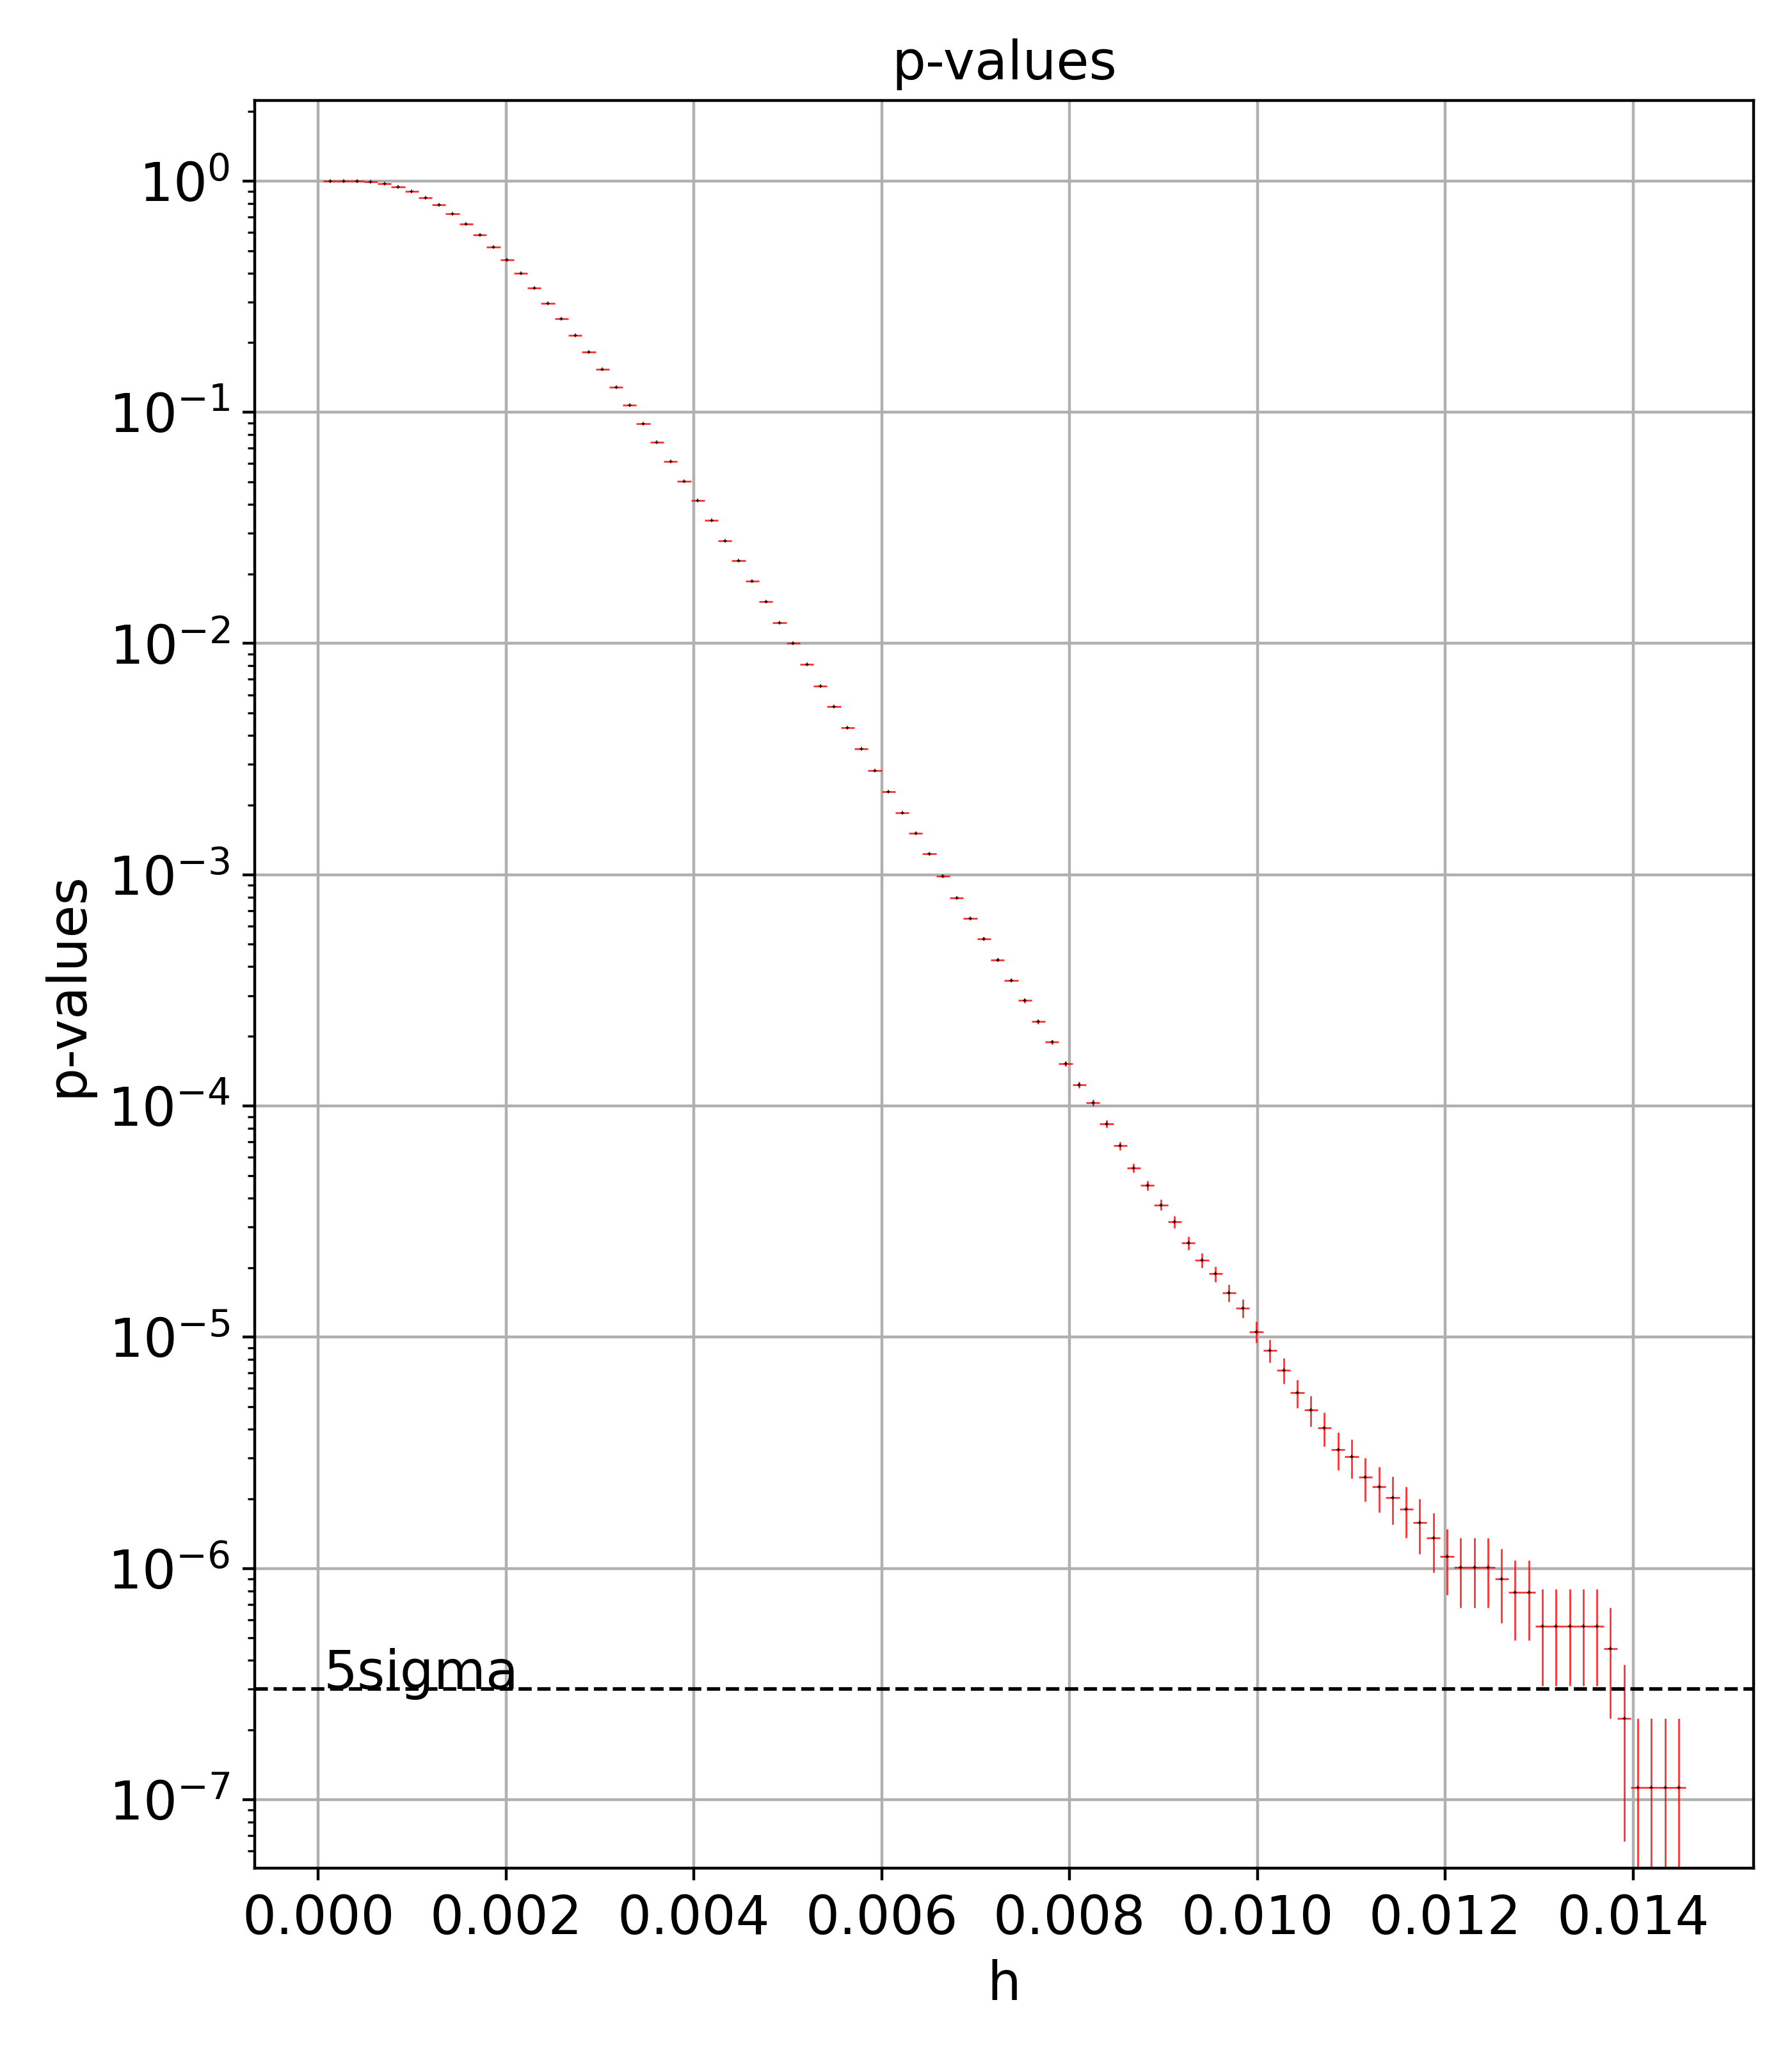
\includegraphics[width=0.5\textwidth]{figures/experiments/p_val/model_0/pvalue_bins_100.png}}
    
    \caption{TS distributions and p-values for A.D. cnn implementation for integration time = 1}
    \label{fig:ts-distribution-and-p-values-cnn-it-1}
\end{figure}

\subsection{Performance metrics}
\label{s:Peformance-Metrics}
The Anomaly Detection (CNN and RNN implementations) and Li\&Ma methods have been tested with two different datasets for different integration times. In the short-term analysis settings, the integration time is set to 5 seconds, while in the very short-term analysis settings, it is set to 1 second. The time series of lengths equal to 5 have been extracted from the original time series of each simulated trial. We are interested in computing the accuracy and false positive rate. These metrics tell us how many time series have been correctly classified and how many false positives classifications have been issued. This tells us how frequently the same GRB event is detected during its evolution. Another performance metric that we want to compute is the average time of the first $5\sigma$ detections for each GRB event and the number of detections limiting the observation duration (from $T_grb_start$ to $T_max$). Since A.D. method can infer each $IT$ seconds of data, while Li\&Ma needs to wait for at least $IT*TSL$ seconds, we expect the A.D. method to have more detections in the short-term window from the start of the GRB event. Finally, the next section will also a confusion matrix to show how many GRB events are seen by the models respectively to each other. 


\section{Results}
\label{s:Experiment-Results}

\subsection{Accuracy and False Positive Rate}
\label{s:Acc-Fpr}
These metrics tell us how many time series have been correctly classified and how many false positives classifications have been issued. This tells us how frequently the same GRB event is detected during its evolution.
Table [ref] shows these metrics for the A.D. CNN and RNN models and for different integration times, 1 and 5 seconds.

\subsection{Serendipitous discoveries use case}
\label{s:Serendipitous-Discoveries-Results}
In the scenario, the GRB event must be detected as soon as possible to broadcast a science alert to other observatories to observe the same event to enable multi-wavelength and multi-messenger analysis. 

Table~\ref{tab:Experiment-Results-E-IT-5} shows the total number of 5$\sigma$ detections performed by the two methods of A.D. and LiMa and the average time in seconds to detect a source for the first time. This time is measured starting from the trigger time that defines the start of the GRB event and not from the start of the observation.

The table shows the LiMa's robust predictions since it detected most GRBs. The A.D. method performs less robust but faster detections since it can predict every $T$ seconds. In LiMa the temporal bins must be independent and the slower prediction rate is 1  every $T*TSL$ seconds. This metric can be broken down further.


\begin{table}[ht]
\centering % used for centering table
\begin{tabular}{l c c c c} % centered columns (4 columns)
\hline\hline %inserts double horizontal lines
Model & Test Set & A.D. (CNN) & A.D. (RNN) & Li\&Ma \\ [0.5ex] % inserts table
%heading
\hline % inserts single horizontal line
Total detections & E & 128 & 143 & 161 \\ 
Accuracy & E &  68.09\% & 76.06\% & 85.64\%  \\ 
Against Li\&Ma & E &  0 & 1 & - \\ 
Mean time first detection & E &  50.74 & 47.48 & 52.02  \\ [1ex] % [1ex] adds vertical space

\hline % inserts single horizontal line
Total detections & H &  174 & 237 & 294 \\
Accuracy & H & 41.23\% & 56.16\% & 69.66\%  \\ 
Against Li\&Ma & H & 2 & 13 & - \\  
Mean time first detection & H & 52.64 s & 61.81 s & 63.18 s \\ [1ex]   

\hline %inserts single line
\end{tabular}
\caption{Result on Test Set E and Test Set H with integration time = 5: Total number of 5$\sigma$ detections performed by the two methods of A.D. and LiMa and the average time in seconds the methods took to detect a source for the first time, over 188 GRB (E) and 422 GRB (H) trials.}
\label{tab:Experiment-Results-E-IT-5} 
\end{table}



\begin{table}[ht]
\centering % used for centering table
\begin{tabular}{l c c c c} % centered columns (4 columns)
\hline\hline %inserts double horizontal lines
Model & Test Set & A.D. (CNN) & A.D. (RNN) & Li\&Ma \\ [0.5ex] % inserts table
%heading
\hline % inserts single horizontal line
Total detections & E & 128 & 143 & 161 \\ 
Accuracy & E &  68.09\% & 76.06\% & 85.64\%  \\ 
Against Li\&Ma & E &  0 & 1 & - \\ 
Mean time first detection & E &  50.74 & 47.48 & 52.02  \\ [1ex] % [1ex] adds vertical space

\hline % inserts single horizontal line
Total detections & H &  174 & 237 & 294 \\
Accuracy & H & 41.23\% & 56.16\% & 69.66\%  \\ 
Against Li\&Ma & H & 2 & 13 & - \\  
Mean time first detection & H & 52.64 s & 61.81 s & 63.18 s \\ [1ex]   

\hline %inserts single line
\end{tabular}
\caption{Result on Test Set E and Test Set H with integration time = 1 : Total number of 5$\sigma$ detections performed by the two methods of A.D. and LiMa and the average time in seconds the methods took to detect a source for the first time, over 188 GRB (E) and 422 GRB (H) trials.}
\label{tab:Experiment-Results-E-IT-1} 
\end{table}


\begin{figure}[t]
\centering
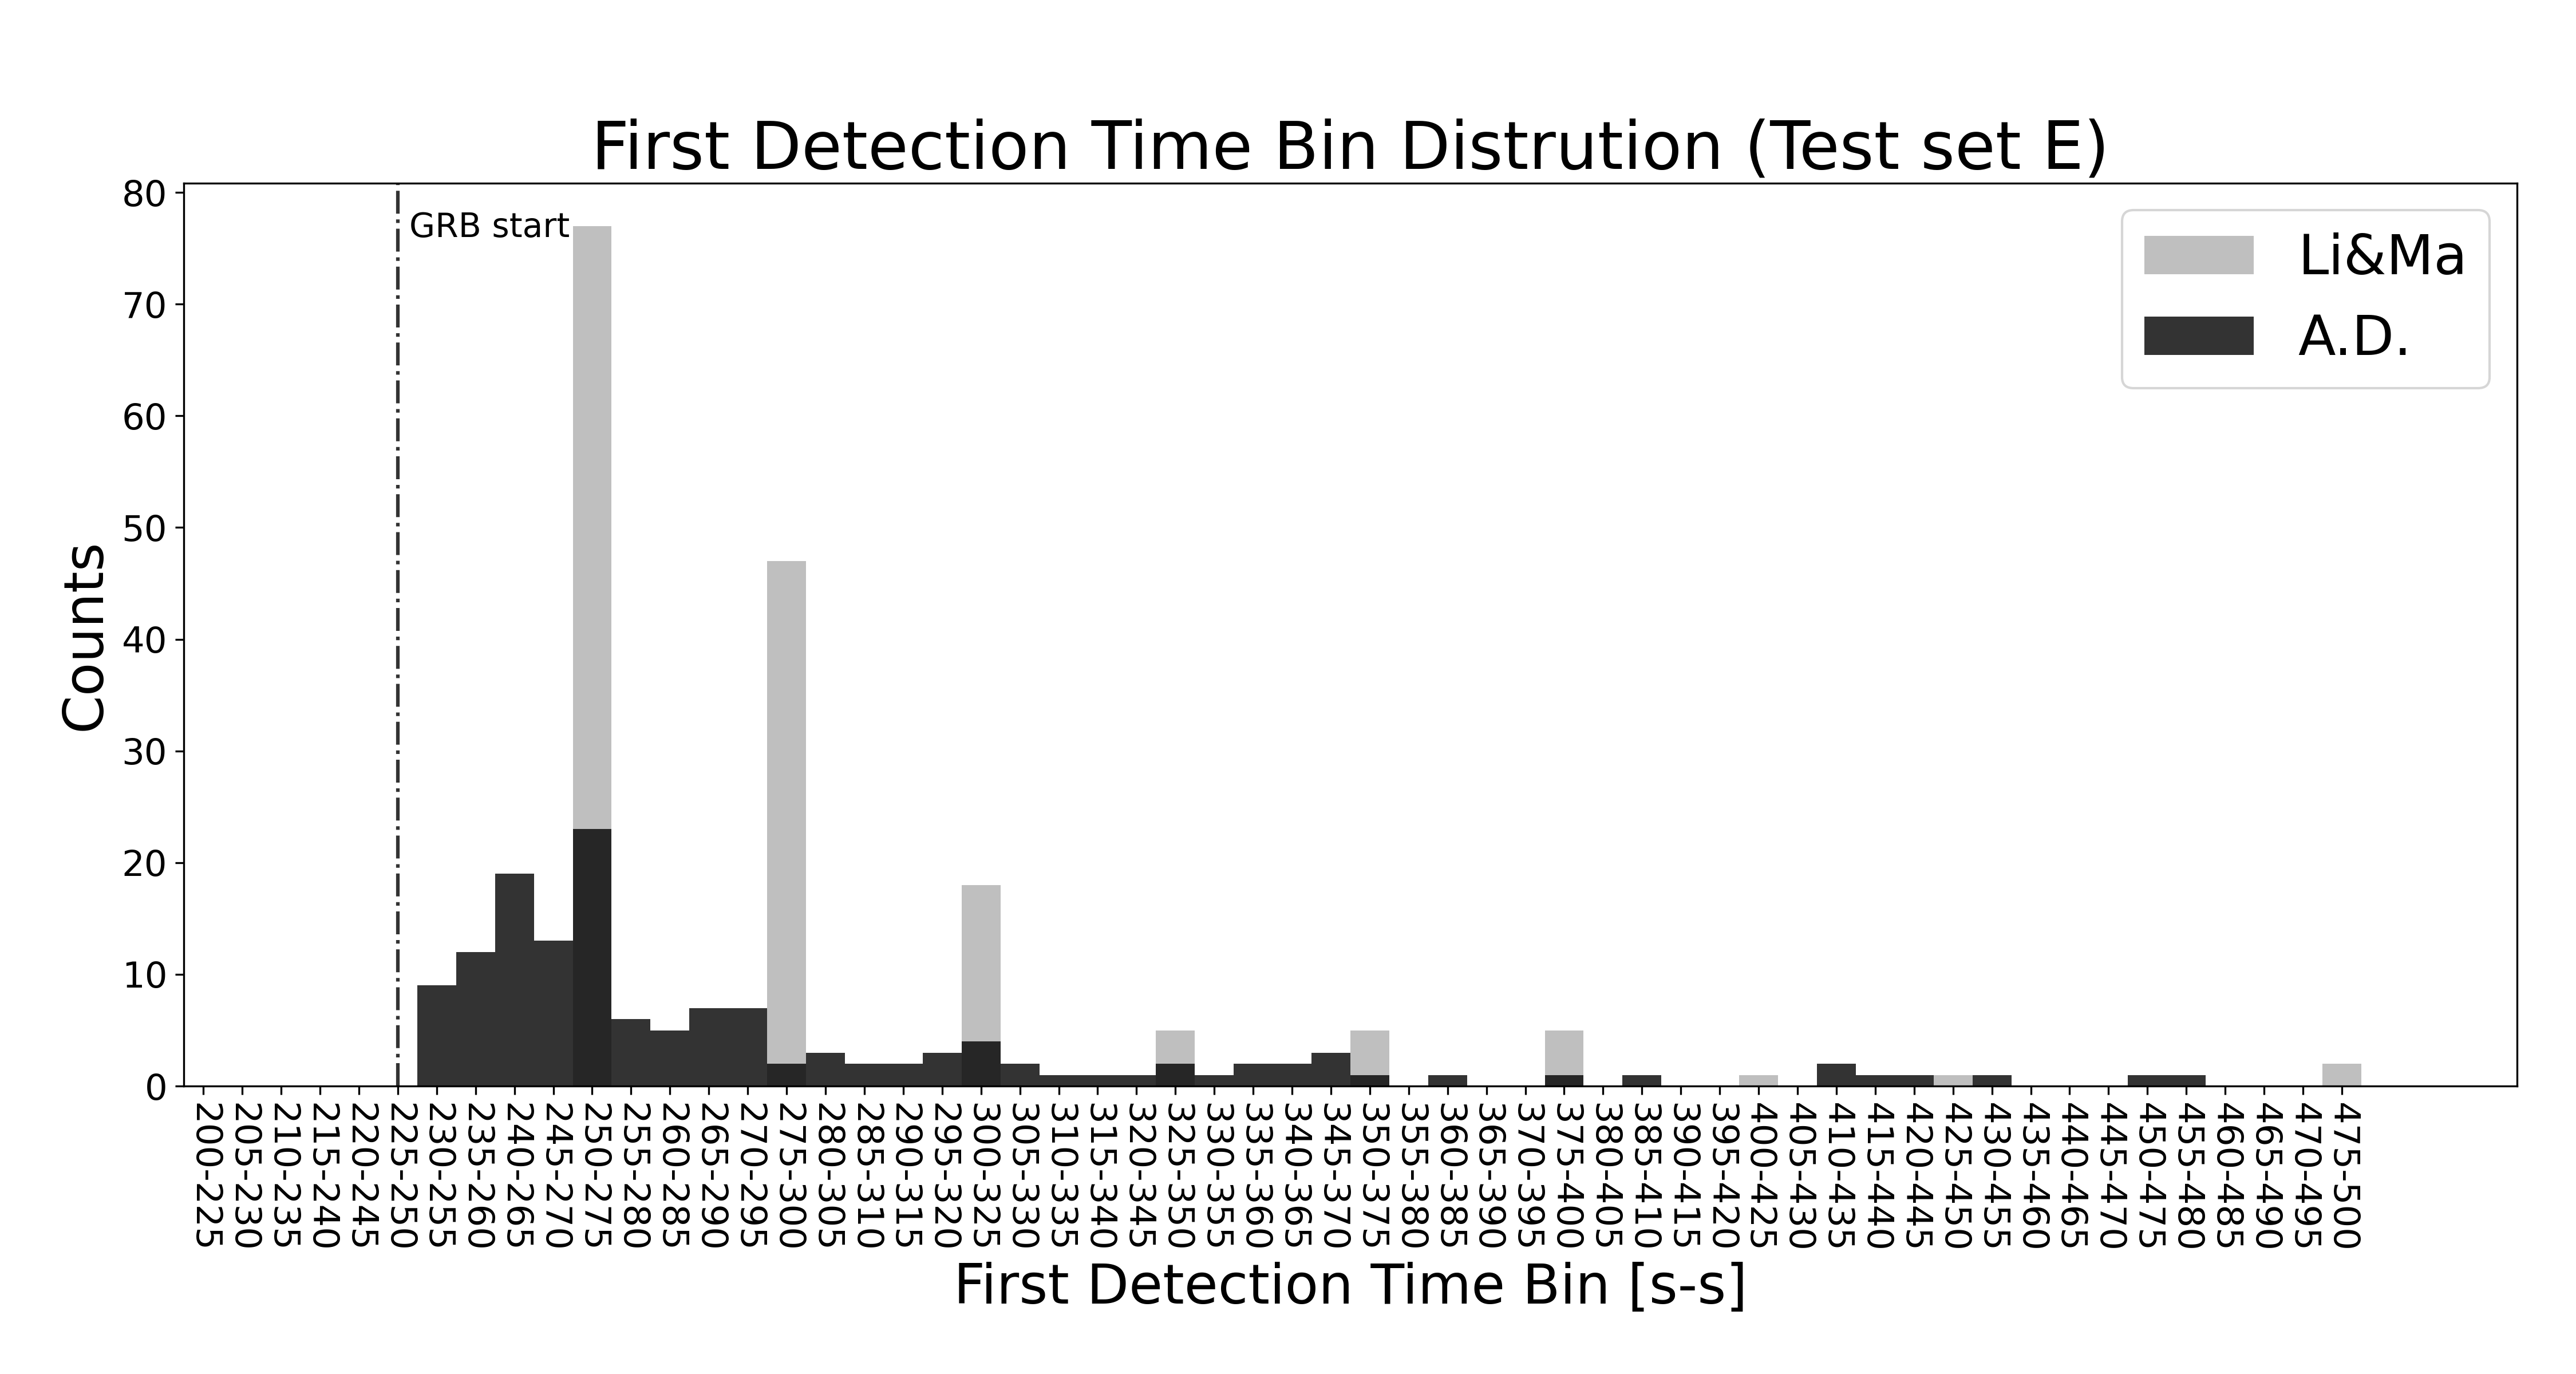
\includegraphics[width=1\textwidth]{figures/experiments/ad_vs_li_ma_first_detections_testset_e_id_1.png}
\caption{Result on Test Set E: 5$\sigma$ detection times distributions for A.D. and LiMa over 188 GRB trials.}
\label{f:ad-vs-lima-first-detection}
\end{figure}


\begin{figure}[t]
\centering
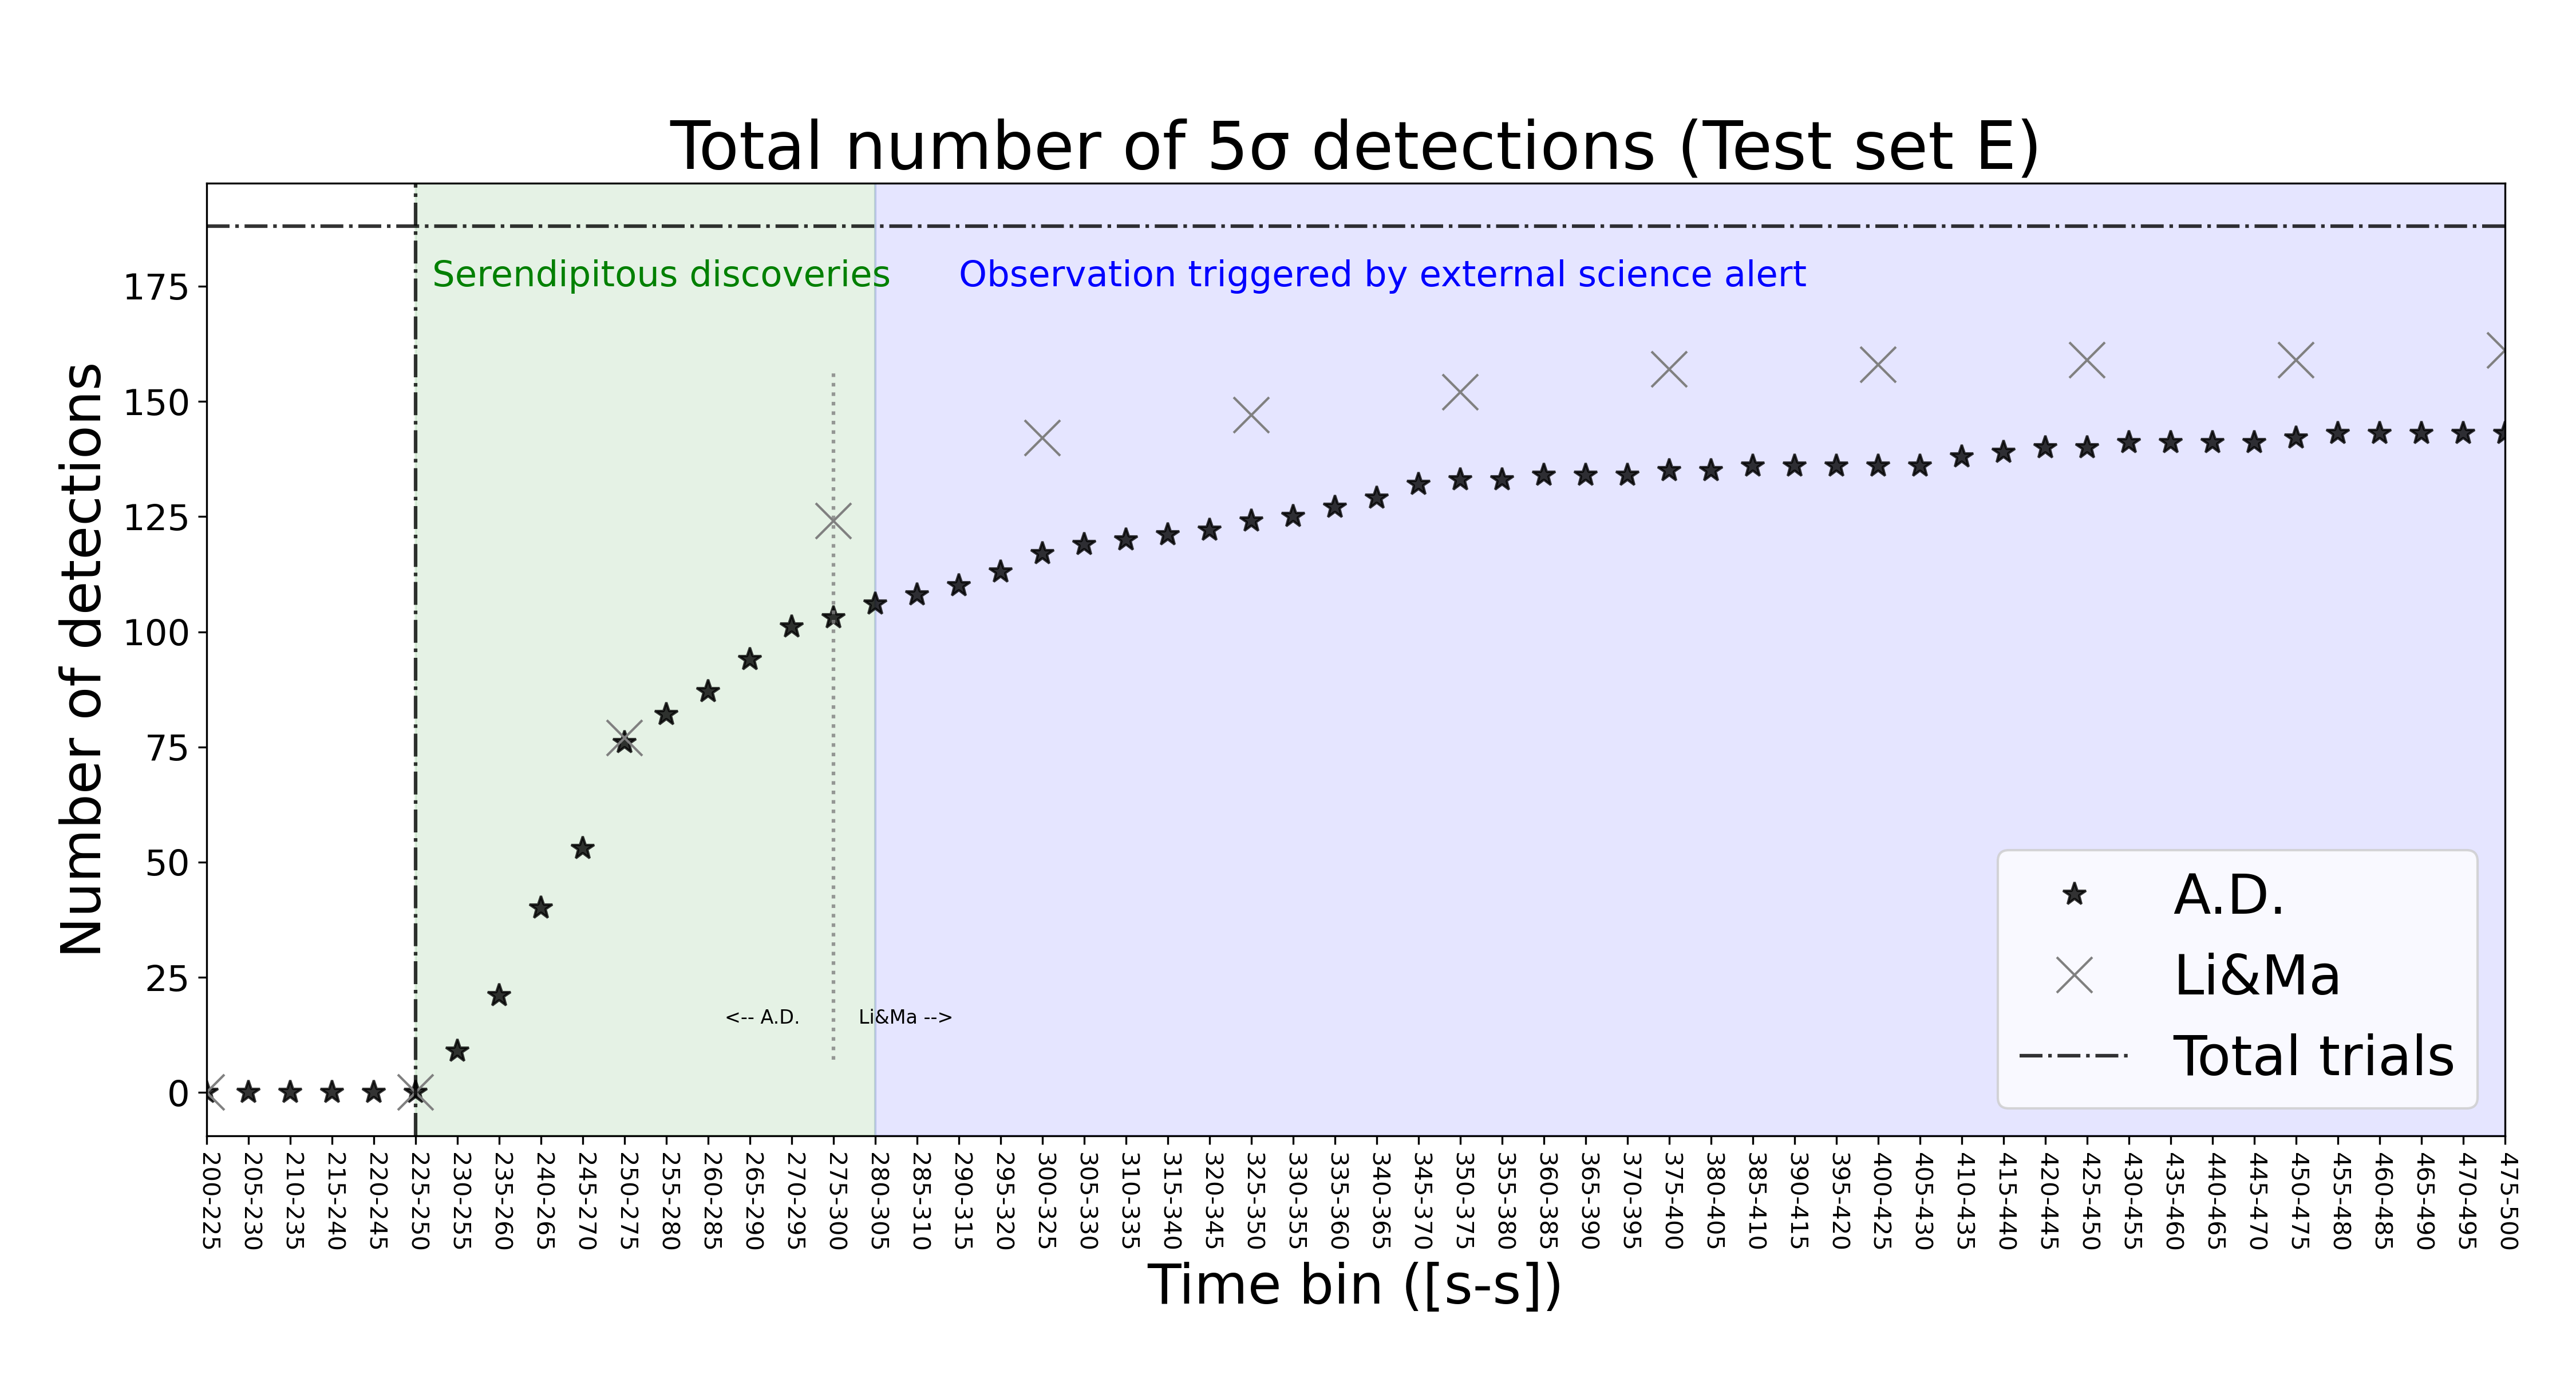
\includegraphics[width=1\textwidth]{figures/experiments/ad_vs_li_cumulative_testset_e_id_1.png}
\caption{Result on Test Set E: Total number of 5$\sigma$ detections (out of 188 GRB trials) performed by the two methods of A.D. and LiMa.}
\label{f:ad-vs-lima}
\end{figure}

\begin{figure}[t]
\centering
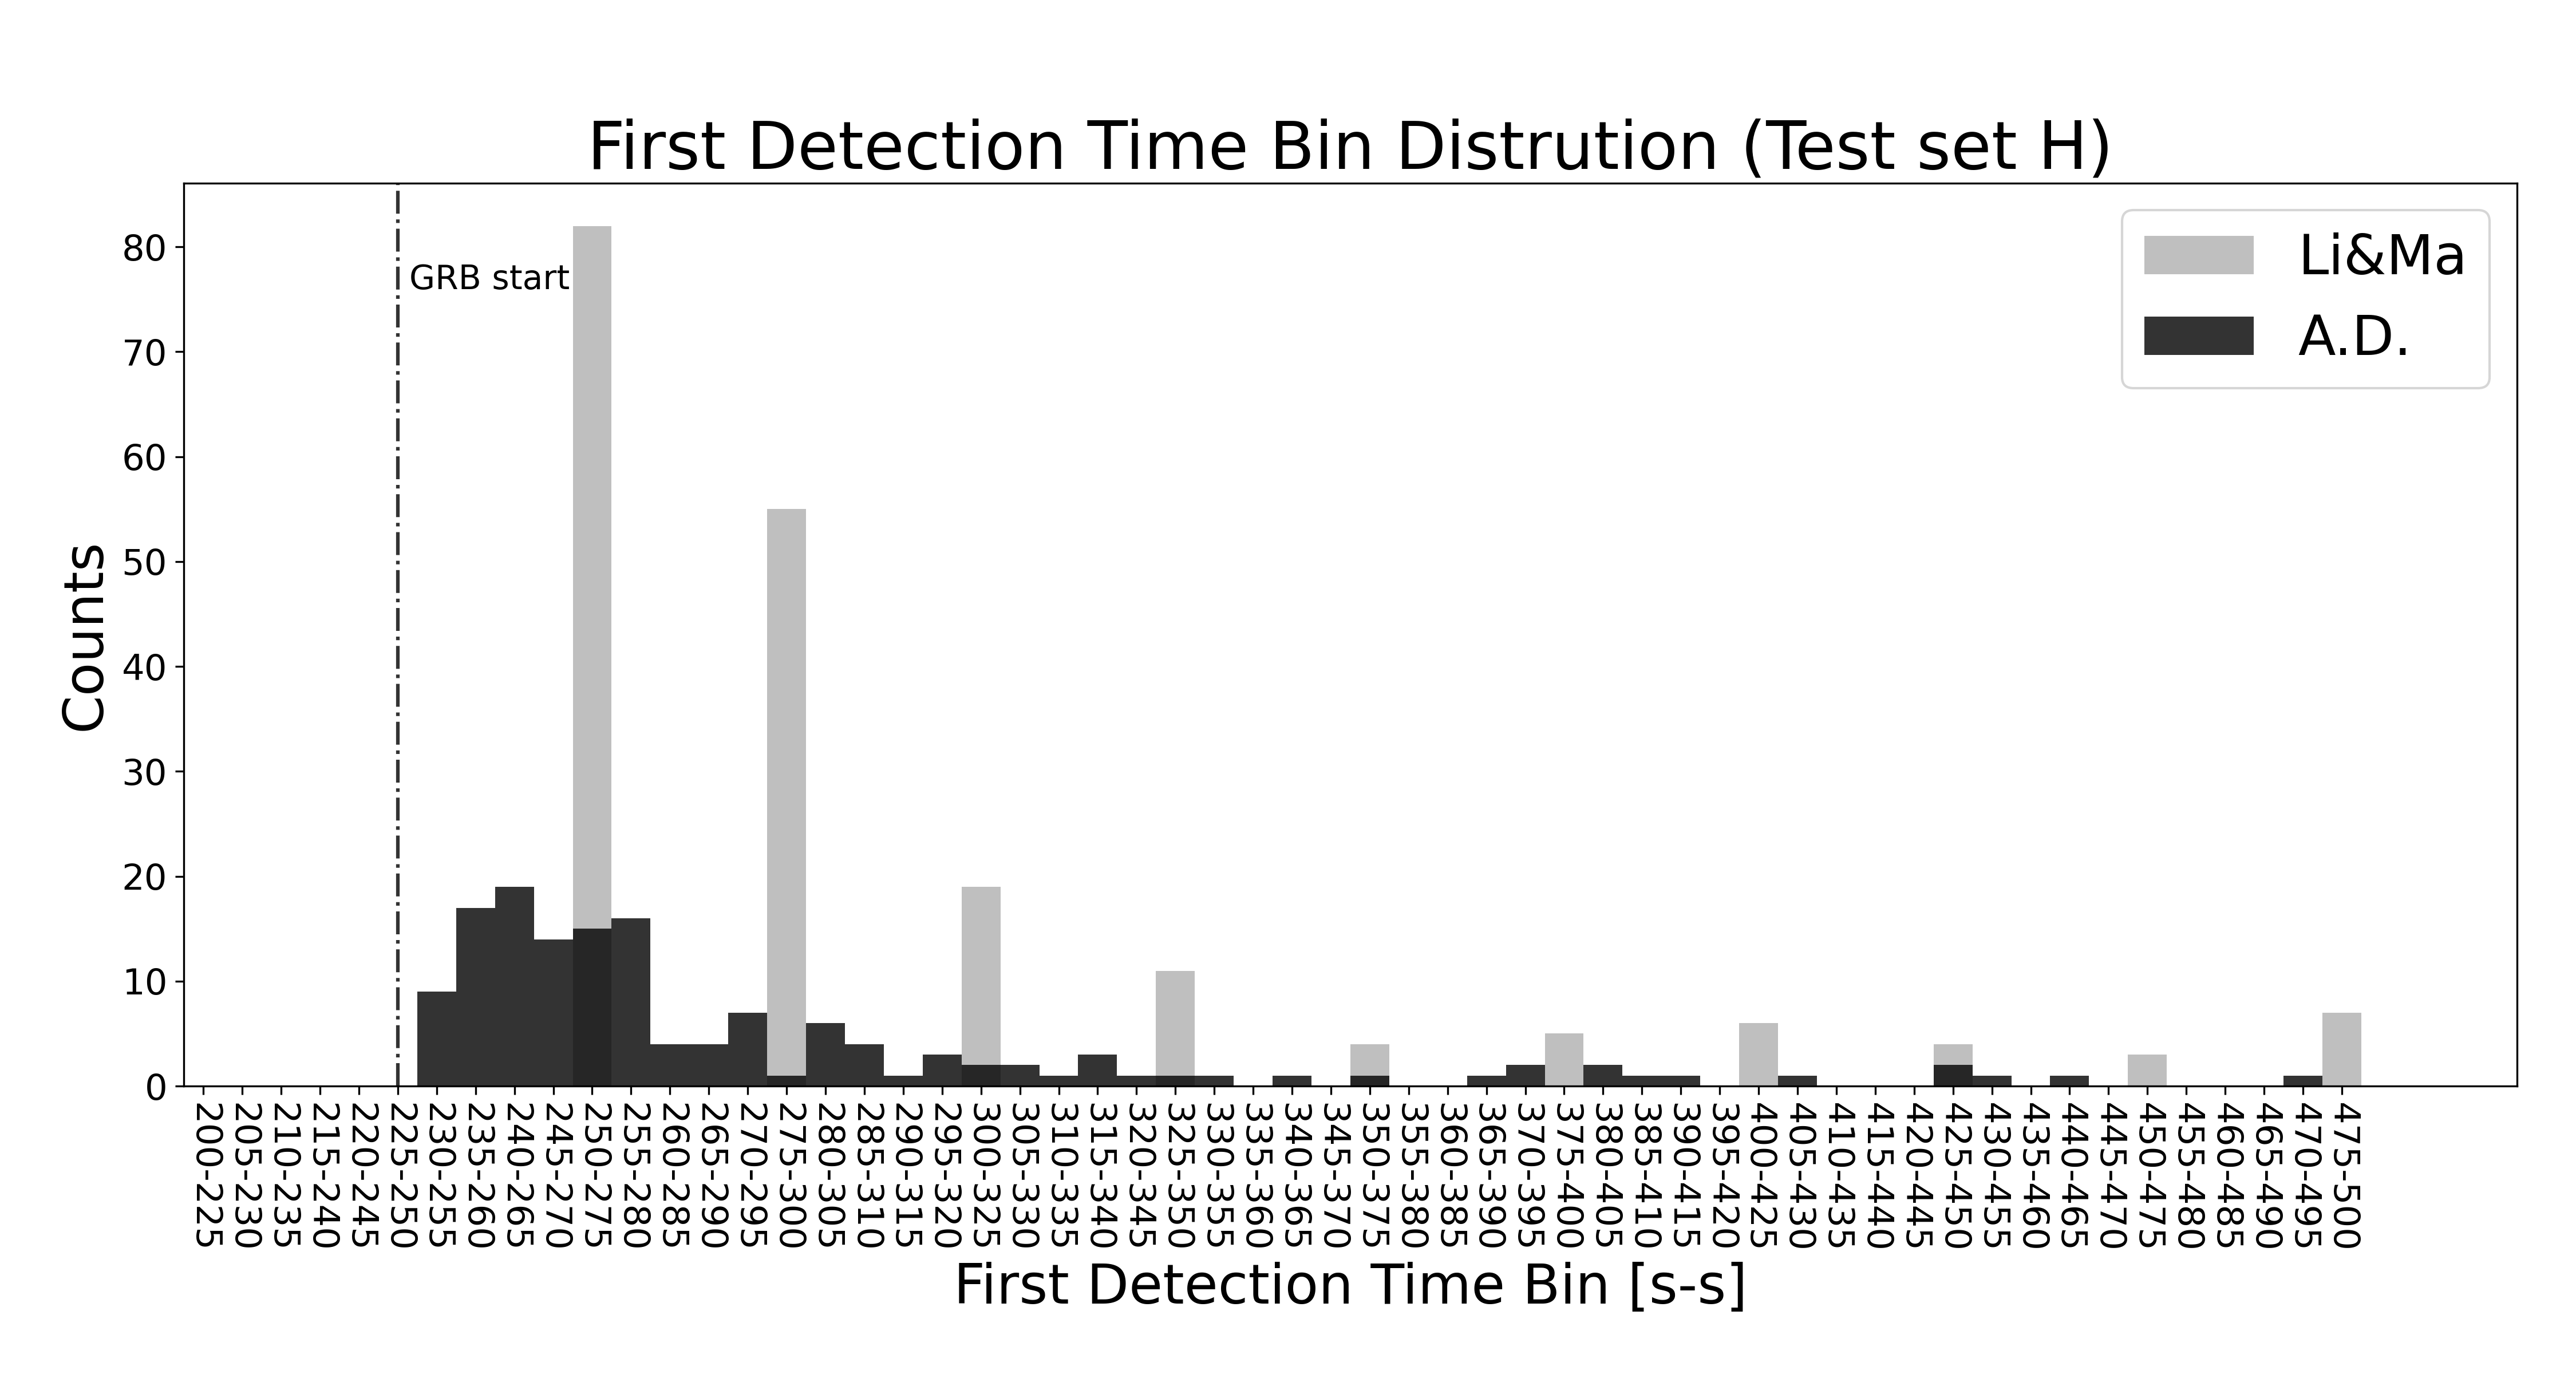
\includegraphics[width=1\textwidth]{figures/experiments/ad_vs_li_ma_first_detections_testset_h_id_1.png}
\caption{Result on Test Set H: 5$\sigma$ detection times distributions for A.D. and LiMa over 419 GRB trials.}
\label{f:ad-vs-lima-first-detection}
\end{figure}


\begin{figure}[t]
\centering
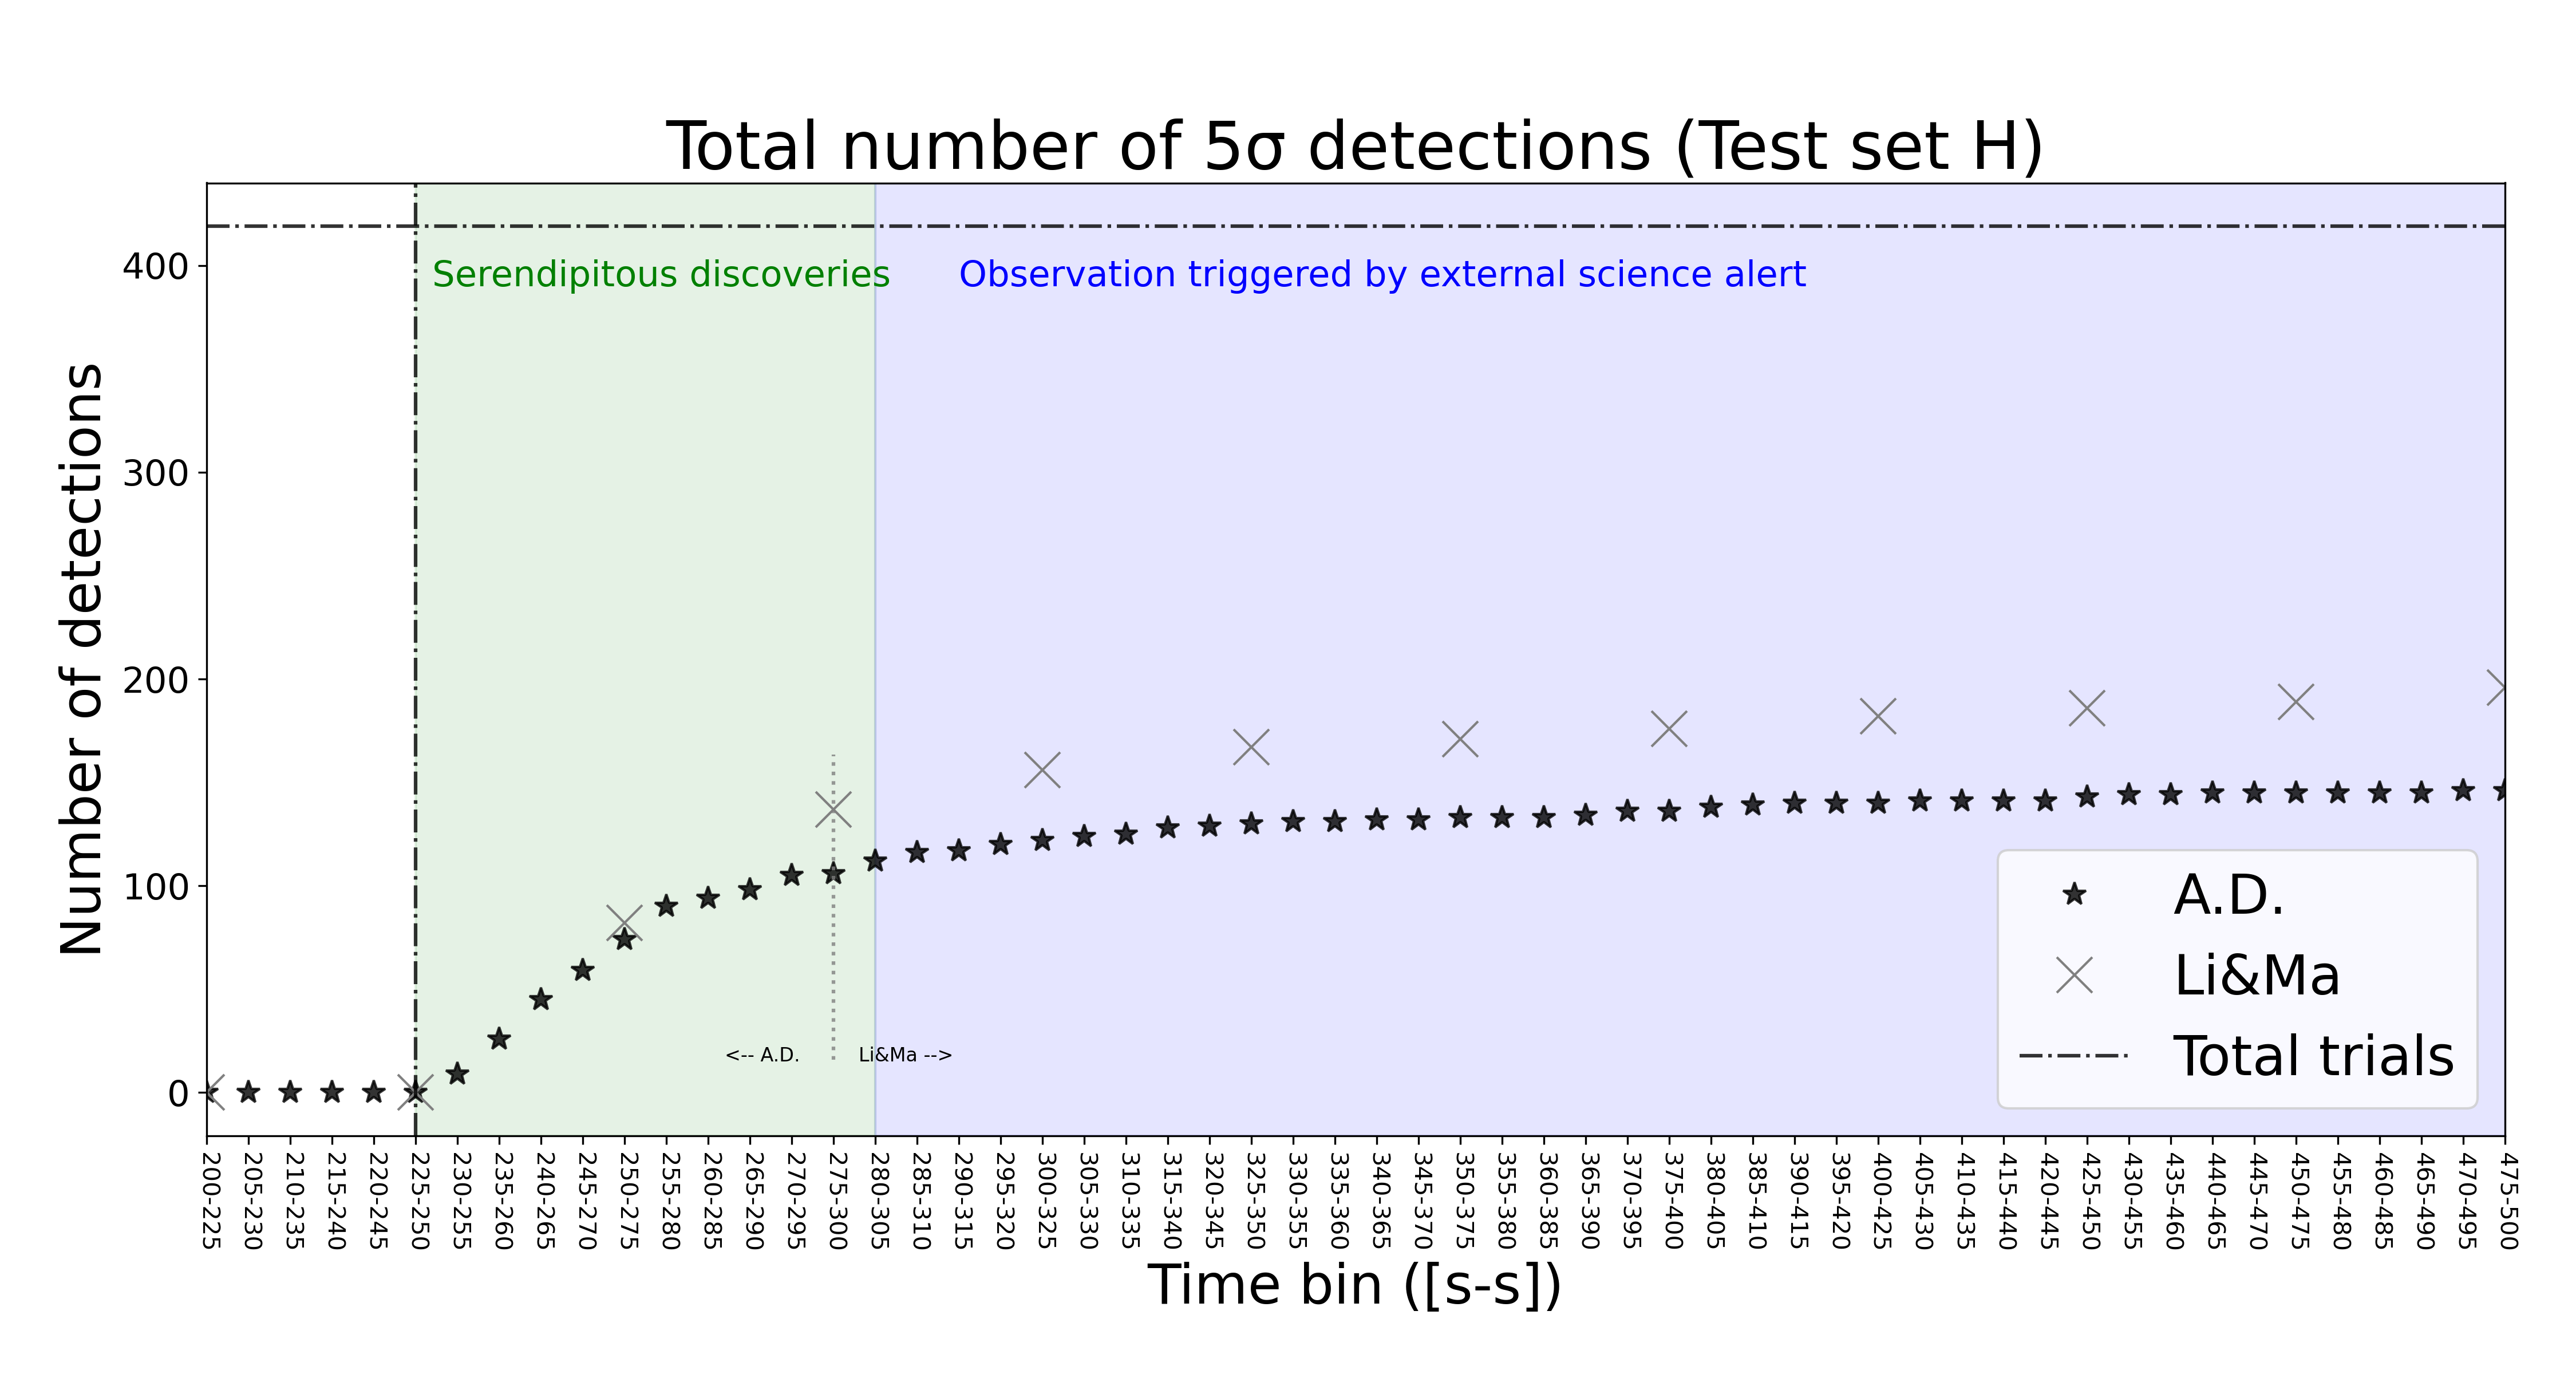
\includegraphics[width=1\textwidth]{figures/experiments/ad_vs_li_cumulative_testset_h_id_1.png}
\caption{Result on Test Set H: Total number of 5$\sigma$ detections (out of 419 GRB trials) performed by the two methods of A.D. and LiMa.}
\label{f:ad-vs-lima}
\end{figure}


Fig~\ref{f:ad-vs-lima-first-detection} and Fig~\ref{f:ad-vs-lima} show the number of predictions at shorter time scales, limiting the duration of the observation. 
% Li&Ma è nel caso peggiore ovvero il bin temporale non sta mai a cavallo dell'onset
The A.D. method is capable of faster prediction on the very short-term temporal scale and the performance of the RNN model, are always better against Li\&Ma. 
 











\subsection{Science alert use case}
\label{s:Science-Alert-Results}
The science-alert use case further limits the time domain. When the observatory reacts to a science alert, its telescopes will change their pointing to observe a sky region in which the GRB event is already started. The time taken to change the pointing is considered fixed and equal to 30 seconds.  



\begin{figure}
    
    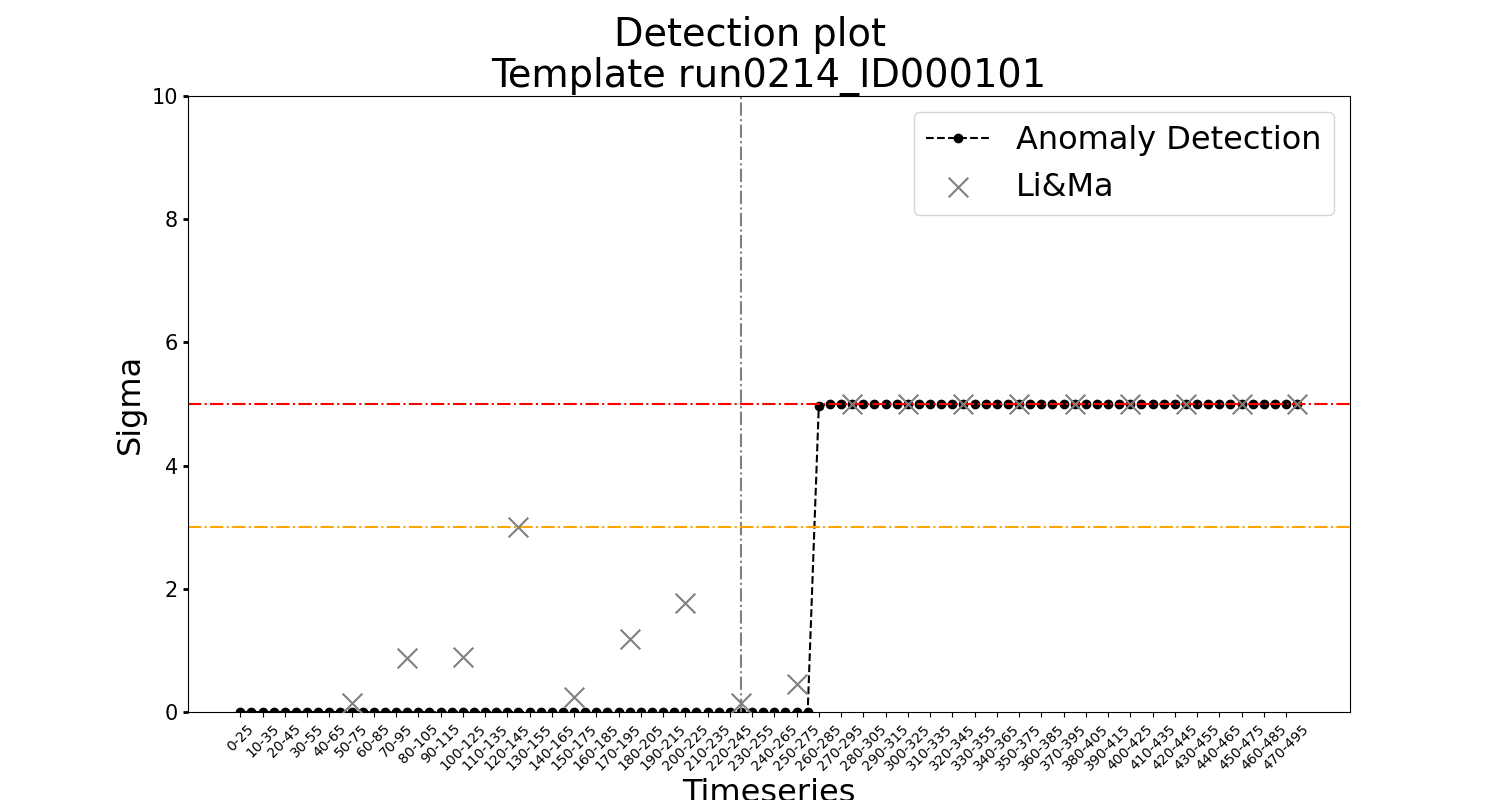
\includegraphics[width=1\textwidth]{figures/experiments/detection_plots/detection_plot_run0214_ID000101_testset_e.png}\hfill
    \\[\smallskipamount]
    
    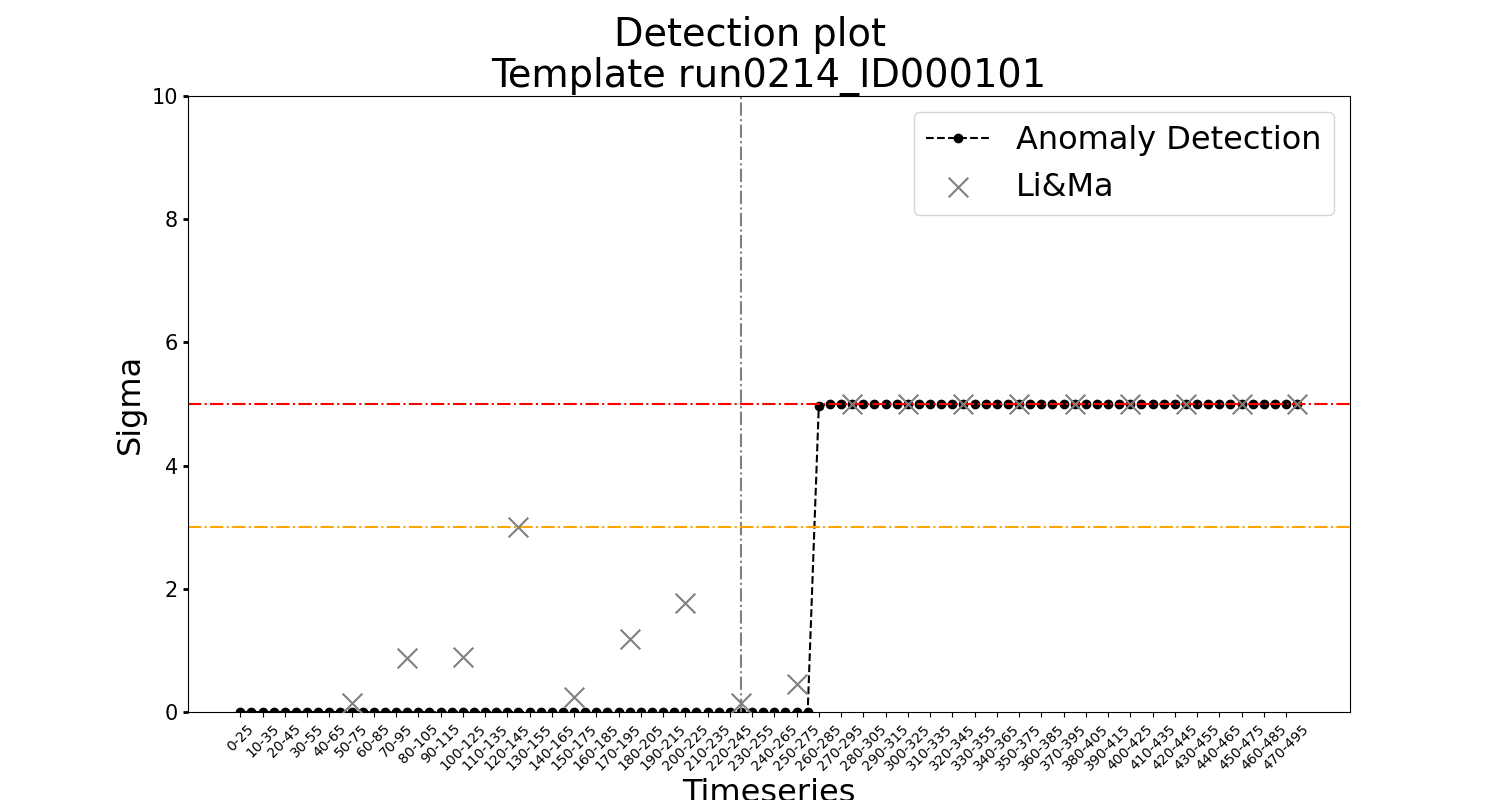
\includegraphics[width=1\textwidth]{figures/experiments/detection_plots/detection_plot_run0214_ID000101_testset_e.png}\hfill
    \\[\smallskipamount]

    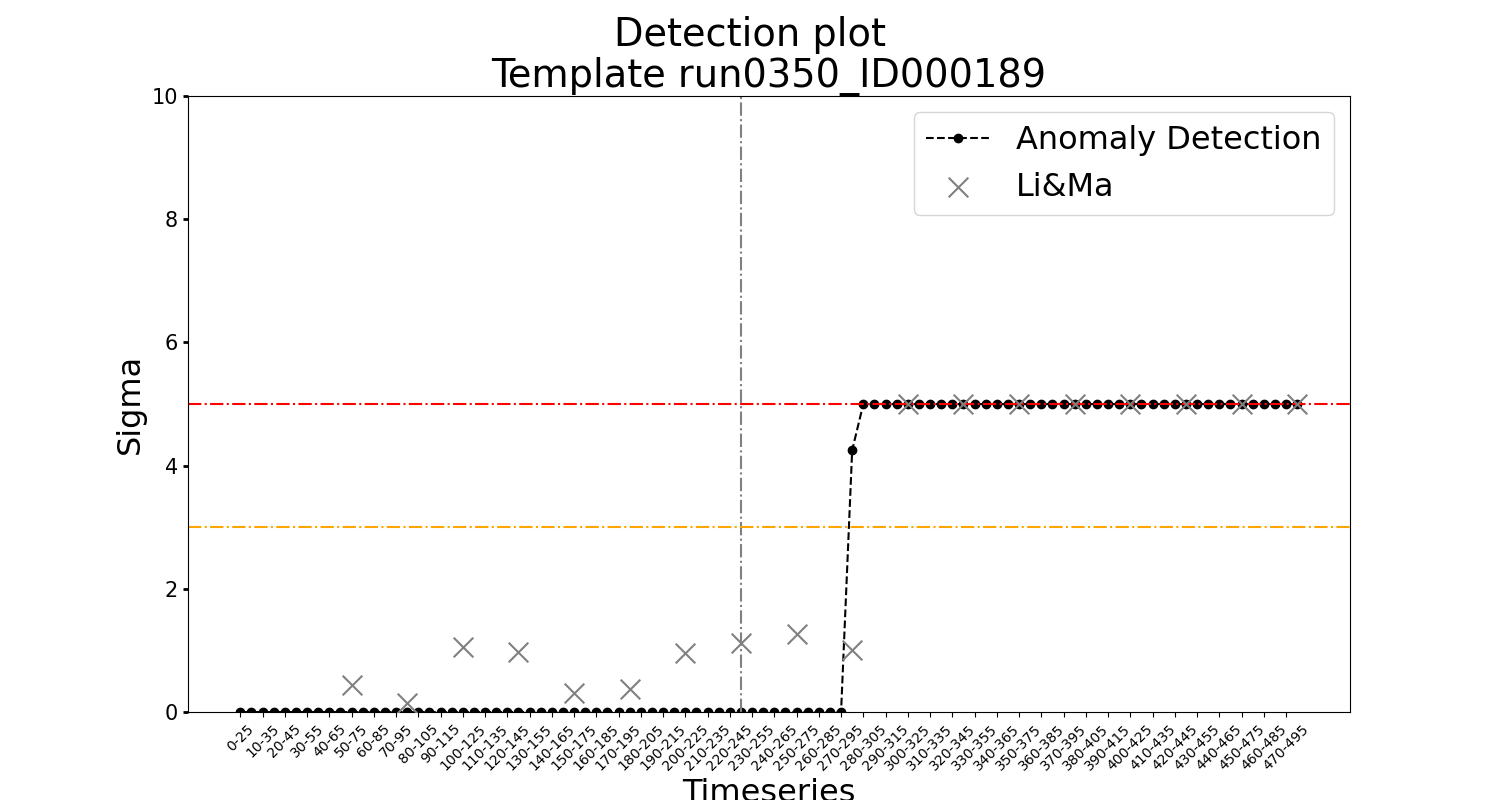
\includegraphics[width=1\textwidth]{figures/experiments/detection_plots/detection_plot_run0350_ID000189_testset_e.png}\hfill
    \\[\smallskipamount]

    \caption{Detection plots 1}\label{fig:detection-plots-1}
\end{figure}


\begin{figure}
    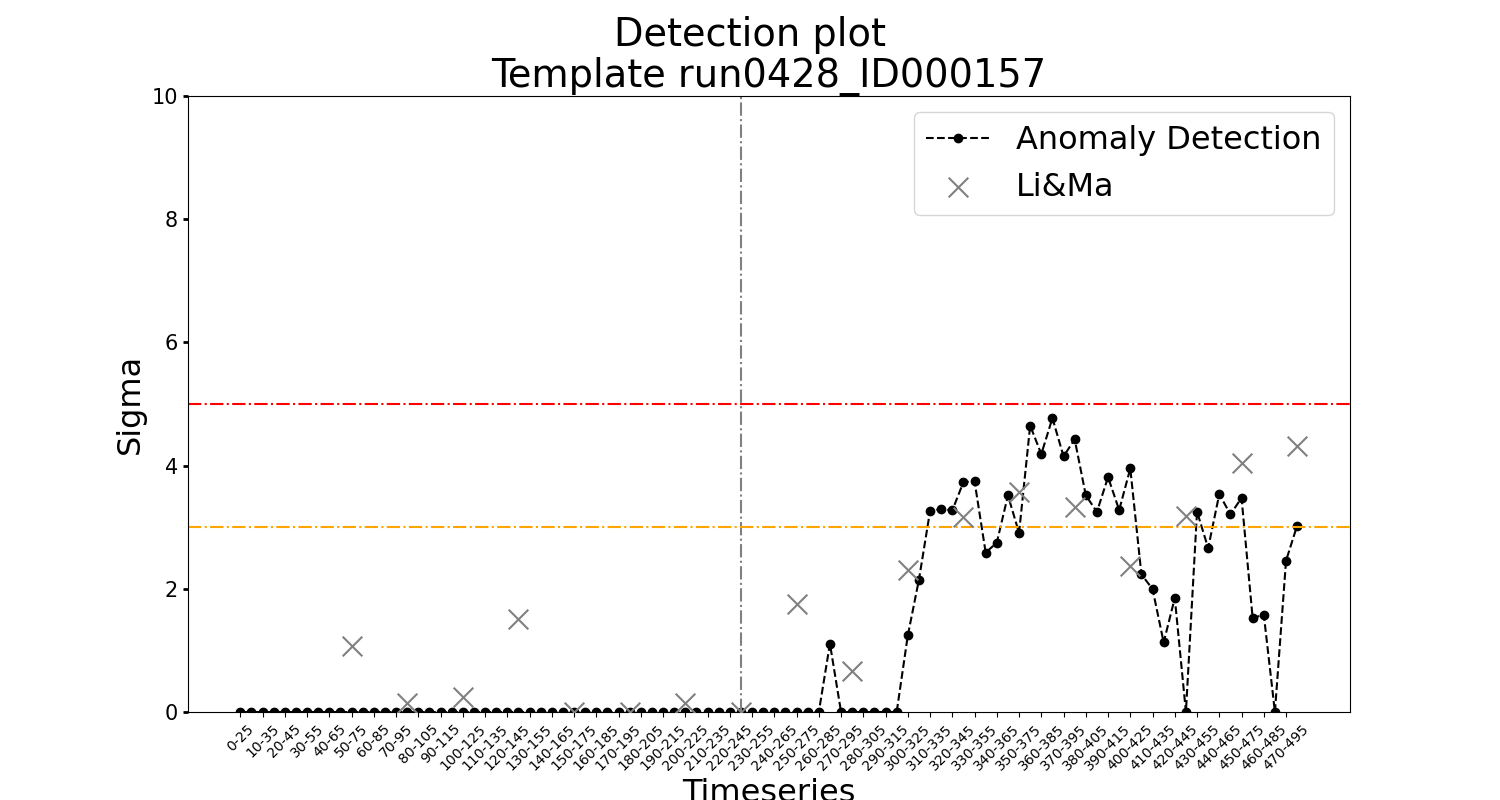
\includegraphics[width=1\textwidth]{figures/experiments/detection_plots/detection_plot_run0428_ID000157_testset_e.png}\hfill
    \\[\smallskipamount]

    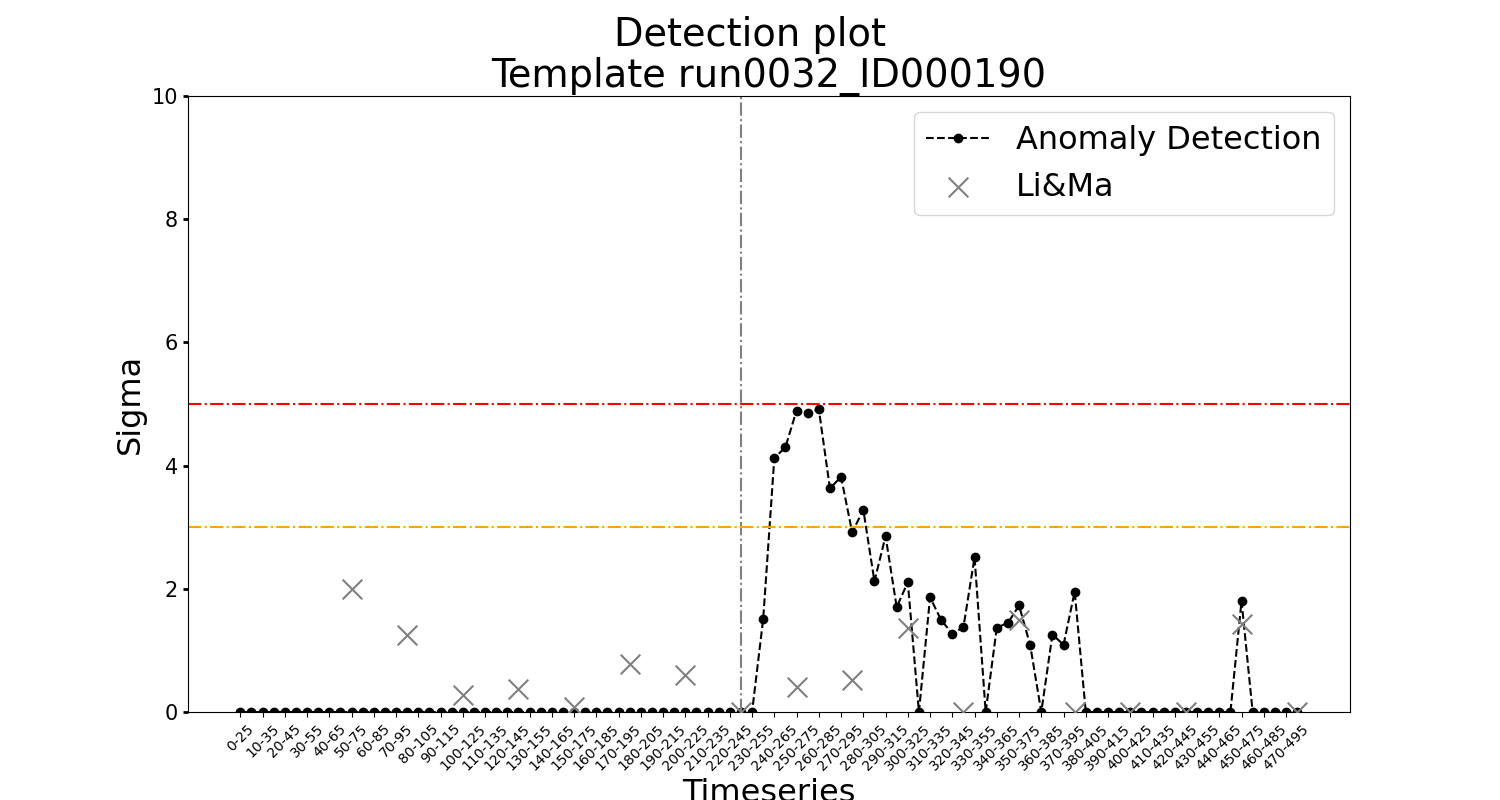
\includegraphics[width=1\textwidth]{figures/experiments/detection_plots/detection_plot_run0032_ID000190_testset_e.png}\hfill
    \\[\smallskipamount]
    
    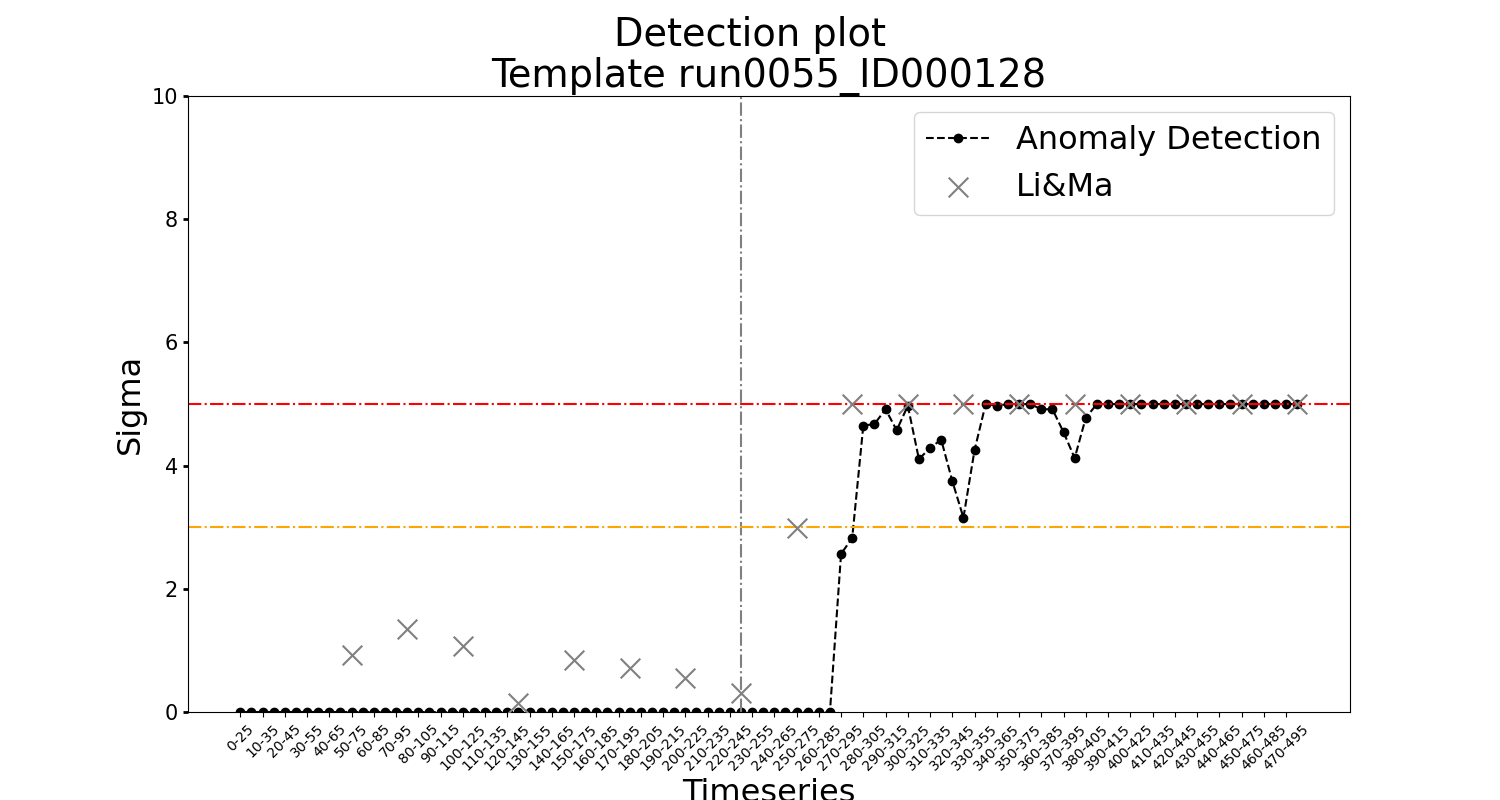
\includegraphics[width=1\textwidth]{figures/experiments/detection_plots/detection_plot_run0055_ID000128_testset_e.png}\hfill
    \\[\smallskipamount]
    \caption{Detection plots 2}\label{fig:detection-plots-2}
\end{figure}



\begin{figure}
    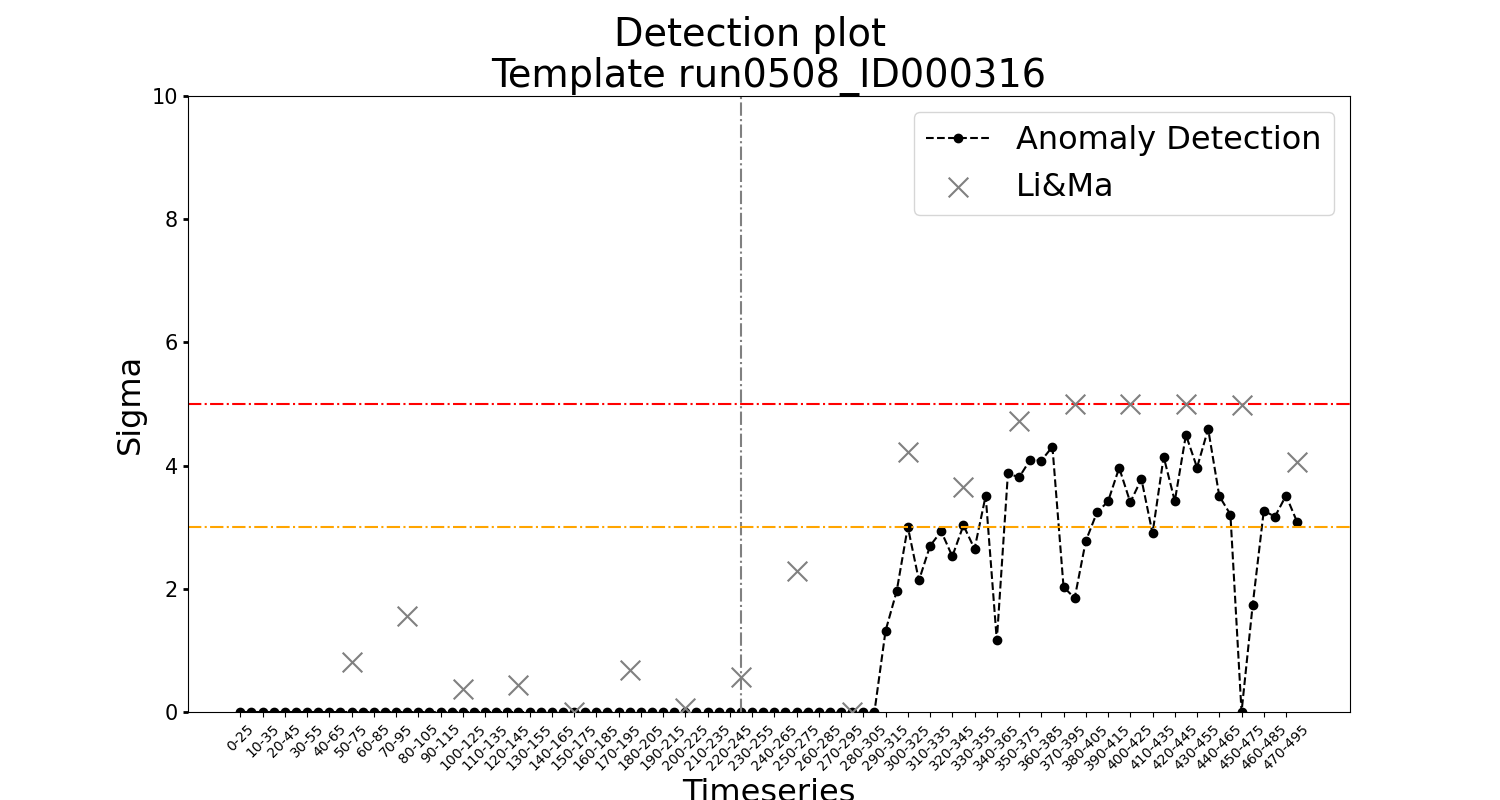
\includegraphics[width=1\textwidth]{figures/experiments/detection_plots/detection_plot_run0508_ID000316_testset_e.png}\hfill
    \\[\smallskipamount]

    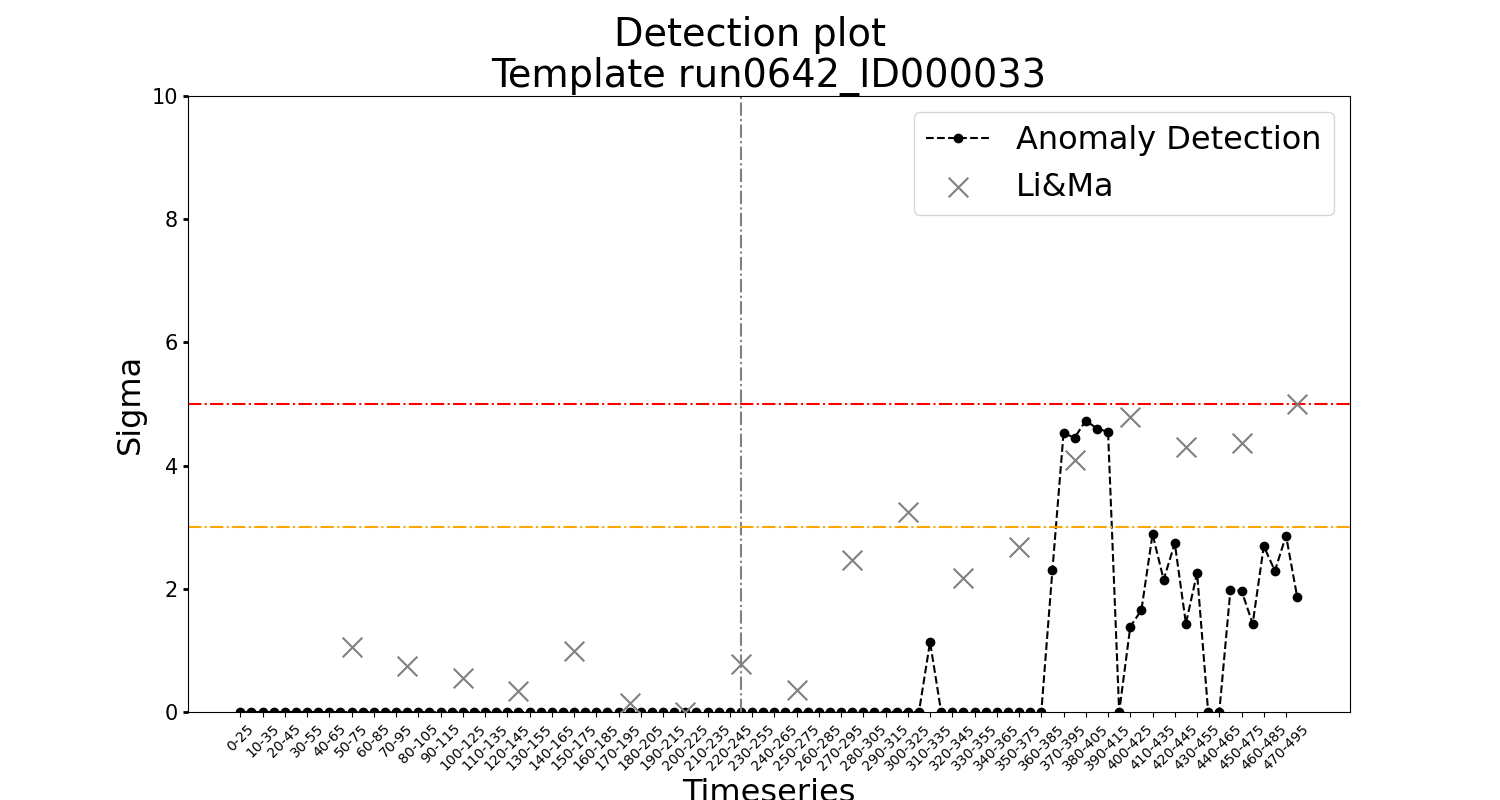
\includegraphics[width=1\textwidth]{figures/experiments/detection_plots/detection_plot_run0642_ID000033_testset_e.png}\hfill
    \\[\smallskipamount]
    
    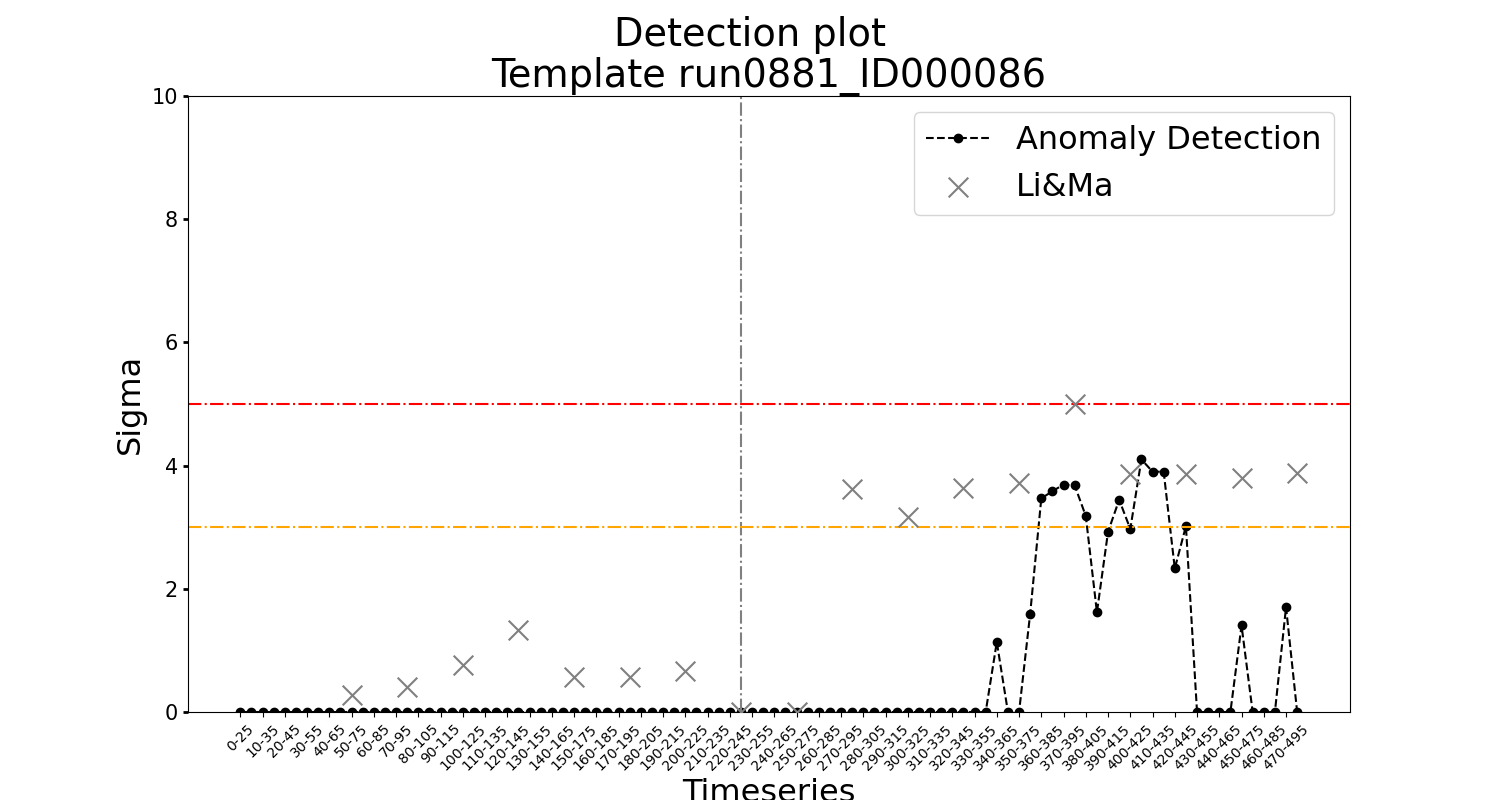
\includegraphics[width=1\textwidth]{figures/experiments/detection_plots/detection_plot_run0881_ID000086_testset_e.png}\hfill
    \\[\smallskipamount]
    \caption{Detection plots 2}\label{fig:detection-plots-2}
\end{figure}

\section{Summary}
\label{s:Experiments-Summary}

Summarize the key findings of the experiments you conducted.

  
  %\chapter{Conclusions}\label{c:Conclusions}
  %\hinttext{!!!ACTION REQUIRED!!!}
\hinttext{The structure I defined is generic and will most likely have to be adapted. I suggest that you skim through the pages and then clear the files \texttt{text/ch2.tex} to \texttt{text/ch7.tex} before you start writing.}

\noindent Optional: Talk about the general development of the respective field of research during your candidature. Talk about how this influenced your work.

\section{Major Contribution 1}

What are the major thoughts and findings discussed in this thesis with respect to \autoref{c:Contribution-1}? How does your research advance the current state-of-the-art? Make sure that you do NOT simply repeat the summary of that chapter.

\section{Major Contribution 2}

What are the major thoughts and findings discussed in this thesis with respect to \autoref{c:Contribution-2}? How does your research advance the current state-of-the-art? Make sure that you do NOT simply repeat the summary of that chapter.


\section{Outlook and Future Work}

Give an outlook regarding your expectations for the overall development of your chosen field of research. List topics that were not covered by your work. Identify and discuss potential avenues for follow-up research that you would consider worthwhile pursuing.
  
  \cleardoublepage
  \appendix
  
  \singlespacing
  %% Bibliography
\label{app:Bibliography} % Reference the bibliography elsewhere with \autoref{app:Bibliography}

\manualmark % Work-around to have small caps also here in the headline
\markboth{\spacedlowsmallcaps{\bibname}}{\spacedlowsmallcaps{\bibname}} % Work-around to have small caps also
%\phantomsection
\refstepcounter{dummy}

\addtocontents{toc}{\protect\vspace{\beforebibskip}} % Place the bibliography slightly below the rest of the document content in the table of contents
\addcontentsline{toc}{chapter}{\tocEntry{\bibname}}
\printbibliography
  \cleardoublepage
  
  \pagestyle{empty}
  \onehalfspacing
  \hfill
\vfill
\section*{Colophon}

\hinttext{This page is entirely optional. However, credit should be given where it is due. Please make sure that you attribute the work of others appropriately.}

This document was authored using \texttt{TeXstudio}\footnote{\url{https://www.texstudio.org}} and typeset based on the \texttt{La Trobe PhD Thesis Template}\footnote{\url{https://github.com/bashimao/ltu-thesis}} (customization of the \texttt{classicthesis}\footnote{\url{https://bitbucket.org/amiede/classicthesis}} \LaTeX{} template) using \texttt{TeX~Live}\footnote{\url{https://tug.org/texlive}} on a machine running \texttt{LinuxMint}\footnote{\url{https://linuxmint.com}}. Other notable software tools used during the production of this document:
\texttt{GNU~Octave}\footnote{\url{https://www.gnu.org/software/octave}} and \texttt{LibreOffice}\footnote{\url{https://www.libreoffice.org}} for number crunching; \texttt{GIMP}\footnote{\url{https://www.gimp.org}} and \texttt{Inkscape}\footnote{\url{https://inkscape.org}} for working with graphics; \texttt{Mendeley Desktop}\footnote{\url{https://www.mendeley.com}} for reference management.\\

\bigskip


\end{document}